%% BEAMER THEME FLIP 2012: Main tex file for compiling
%$ Compile this file. 
%%
%% Copyright 2012 by Flip Tanedo
%% This file may be distributed and/or modified
%% 	1. under the LaTeX Project Public License and/or
%% 	2. under the GNU Public License.
%% 
%% If you e-mail Flip (pt267@cornell.edu) to say that you
%% like this style file, then it would make him smile.

%% Please see notes.txt for comments on Beamer Theme Flip 2013
%% By default, this template is meant to be run with XeLaTeX (for fonts)
%% To run in PDFLaTeX, remove fontspec and any font commands

%% Discussion of Beamer vs XeLaTeX vs LuaLaTeX
%% http://tex.stackexchange.com/questions/29497/xelatex-preventing-beamer-from-using-different-backgrounds



\documentclass[12 pt]{beamer}
\usetheme[
	bullet=circle,		% Other option: square
	bigpagenumber,		% circled page number on lower right
	topline=true,			% colored bar at the top of the frame 
	shadow=false,			% Shading for beamer blocks
	watermark=BG_lower,	% png file for the watermark
	]{Flip}


\newcommand{\titleimage}{title}			% Custom title 
\newcommand{\tanedo}{tanedolight}		% Custom author name
\newcommand{\CMSSMDM}{CMSSMDMlight.png}	% light background plot


%%%%%%%%%%
% FONTS %
%%%%%%%%%%

%% Default font: lmodern, doesn't require fontspec % solves some default warnings
\usepackage[T1]{fontenc}
\usepackage{lmodern}			
%\usepackage{sfmath}		% Sans Serif Math, off by default

%% Protects fonts from Beamer screwing with them
%% http://tex.stackexchange.com/questions/10488/force-computer-modern-in-math-mode
\usefonttheme{professionalfonts}


%% XeLaTeX fonts: (comment out if you don't use XeLaTeX)

%% For advanced fonts: access local OS X fonts
\usepackage[no-math]{fontspec}		
%% This template uses typical OS X and Adobe fonts
\defaultfontfeatures{Mapping=tex-text}	% This seems to be important for mapping glyphs properly

\setmainfont{Gill Sans}			% Beamer ignores "main font" in favor of sans font
\setsansfont{Gill Sans}			% This is the font that beamer will use by default
% \setmainfont{Gill Sans Light}		% Prettier, but harder to read

\setbeamerfont{title}{family=\fontspec{Gill Sans}}


\newcommand{\handwriting}{\fontspec{augie}} % From Emerald City, free font
% \newcommand{\handwriting}{}	% If you prefer no special handwriting font or don't have augie

%% Gill Sans doesn't look very nice when boldfaced
%% This is a hack to use Helvetica instead
%% Usage: \textbf{\forbold some stuff}
\newcommand{\forbold}{\fontspec{Helvetica}}
% \newcommand{\forbold}{} % if you want no special boldface



%%%%%%%%%%%%%%%%%%%%%%%%
% Usual LaTeX Packages %
%%%%%%%%%%%%%%%%%%%%%%%%
\usepackage[utf8]{inputenc}
\usepackage{epstopdf}
\usepackage{amsmath}
\usepackage{amsfonts}
\usepackage{amssymb}
\usepackage{graphicx}
\usepackage{mathrsfs} 			% For Weinberg-esque letters
\usepackage{cancel}				% For "SUSY-breaking" symbol
\usepackage{slashed}            % for slashed characters in math mode
\usepackage{bbm}                % for \mathbbm{1} (unit matrix)
\usepackage{amsthm}				% For theorem environment
\usepackage{multirow}			% For multi row cells in table
\usepackage{arydshln} 			% For dashed lines in arrays and tables
\usepackage{tikzfeynman}		% For Feynman diagrams
% \usepackage{subfig}           % for sub figures
% \usepackage{young}			% For Young Tableaux
% \usepackage{xspace}			% For spacing after commands
% \usepackage{wrapfig}			% for Text wrap around figures
% \usepackage{framed}
\usepackage{pgf,pgfpages}
\usepackage{units}
\usepackage{booktabs}
\usepackage{color}
\usepackage{subfigure}
\usepackage{setspace}
\usepackage{epstopdf}
\usepackage{booktabs}
\usepackage{enumerate}
\usepackage{array}
\usepackage{geometry}
\usepackage{amsthm}
\usepackage{listings}
\usepackage{wrapfig}
%\usepackage{subfig}
\usepackage{amsfonts}
\usepackage{ mathrsfs }
%\usepackage{csquotes}
%\usepackage[american]{babel}
%\usepackage[english]{babel}
%\usepackage{csquotes}
%\usepackage{biblatex}
\usepackage[backend=bibtex,style=numeric-comp,autocite=superscript,style=authoryear, doi=false, url=false]{biblatex} 
%bibstyle=authoryear,style=authoryear
%
%\usepackage[backend=bibtex,,,style=authoryear]{biblatex} %bibstyle=authoryear,style=authoryear
%bibstyle=authoryear,style=authoryear
\addbibresource{references.bib}
\renewcommand{\bibfont}{\small}
\setbeamerfont{footnote}{size=\tiny}
\usepackage{transparent}
%\usepackage{caption}
%\captionsetup{font=footnotesize}
\setbeamerfont{caption}{size=\scriptsize}
\usepackage{framed}
\usepackage[export]{adjustbox}


\addtobeamertemplate{block begin}{\pgfsetfillopacity{0.9}}{\pgfsetfillopacity{1}}
\addtobeamertemplate{block alerted begin}{\pgfsetfillopacity{0.9}}{\pgfsetfillopacity{1}}
\addtobeamertemplate{block example begin}{\pgfsetfillopacity{0.9}}{\pgfsetfillopacity{1}}
\addtobeamertemplate{footnote}{}{\vspace{2ex}}

%\usepackage{multimedia}
\usepackage{media9}
\addmediapath{Movies/}
\graphicspath{{figures/}}	% Put all images in this directory. Avoids clutter.


\usetikzlibrary{backgrounds}
\usetikzlibrary{mindmap,trees}	% For mind map
% http://www.texample.net/tikz/examples/computer-science-mindmap/


% SOME COMMANDS THAT I FIND HANDY
% \renewcommand{\tilde}{\widetilde} % dinky tildes look silly, dosn't work with fontspec
\newcommand{\comment}[1]{\textcolor{comment}{\footnotesize{#1}\normalsize}} % comment mild
\newcommand{\Comment}[1]{\textcolor{Comment}{\footnotesize{#1}\normalsize}} % comment bold
\newcommand{\COMMENT}[1]{\textcolor{COMMENT}{\footnotesize{#1}\normalsize}} % comment crazy bold
\newcommand{\Alert}[1]{\textcolor{Alert}{#1}} % louder alert
\newcommand{\ALERT}[1]{\textcolor{ALERT}{#1}} % loudest alert
%% "\alert" is already a beamer pre-defined

 \DeclareNameAlias{sortname}{first-last}
 \DeclareCiteCommand{\footcustomcite}{}{%
     \footnote{\textcolor{darkgray}{\printnames[author]{author}}
       \textcolor{darkgray}{(\printfield{year})} 
   %\textcolor{darkgray}{,\printfield{title}. 
    \textcolor{darkgray}{\printfield{journaltitle} \textbf{\printfield{volume}}, \printfield{number}.}}}{;}{}

\author[Julia Rossi \quad {SDSU \& CGU}]{Julia Rossi}
\title[NCVA for NLS Equations and its Applications]{Non-Conservative Variational Approximation for Nonlinear Schr\"{o}dinger Equations and its Applications}
\institute{San Diego State University \& Claremont Graduate University}
\date{\today}



\begin{document}

%%%%%%%%%%%%%%%%%%%%%%%%
% Additional  settings %
%%%%%%%%%%%%%%%%%%%%%%%%

%% To use external nodes; http://www.texample.net/tikz/examples/beamer-arrows/
\tikzstyle{every picture}+=[remember picture]


%%%%%%%%%%%%%%%%%%%%%%%%
% Actual content below %
%%%%%%%%%%%%%%%%%%%%%%%%

%% It's much nicer to have all the content in a separate file
% DO NOT COMPILE THIS FILE DIRECTLY!
% This is included by the the driver file (FlipBeamerTemplate.tex).

{ %% This is a total kludge for a fancy title page background
\setbeamertemplate{sidebar right}{\llap{
\includegraphics[width=\paperwidth,height=\paperheight]{BG_upper}}}
\begin{frame}[c]
\begin{center}
	\vspace{1em}
	\large{\fontspec{Trebuchet MS} \bfseries Non-Conservative Variational Approximations for Nonlinear Schr\"{o}dinger Equations and its Applications} \\ 
	\vspace{3em}
	\textcolor{gray}{Dissertation Defense} \\
	\vspace{1em}
	
	  \normalsize {\fontspec{Trebuchet MS} Julia Rossi } \\ 
	 \vspace{1em}	
	\textcolor{normal text.fg!50!Comment}{May  27, 2016} \\
	\vspace{1em}
	
\includegraphics[height=1cm]{sdsu}
	\quad ~
\includegraphics[height=1cm]{Claremont_Graduate_University_logo}\\

\end{center}
\end{frame}
}



%Slide 1: Overview
 \begin{frame}[c]{Introduction}{Overview}
\begin{itemize}
\item \textcolor{paleblue}{Motivation}
%\pause
\item \textcolor{paleblue}{Variational Approximation} 
%\pause
	\begin{itemize}
	\item Non-conservative VA (NCVA)
	\item Perturbed VA (PVA)
	\end{itemize}
%\pause
\item \textcolor{paleblue}{Applications of NCVA}
%\pause
	\begin{itemize}
	\item NLS with Linear Loss
	%\pause
	\item NLS with Density Dependent Loss
	%\pause
	\item Exciton-Polariton Condensate - NLS with Linear Gain and Density Dependent Loss
	%\pause
	\end{itemize}
%\pause
\item \textcolor{paleblue}{Applications to Spontaneous Symmetry Breaking} 
	\begin{itemize}
		%\item $\mathcal{PT}$-symmetric sG and $\phi^4$
		\item SSB in Passive Kerr Resonator	
		\item NCVA and Local Bifurcation Analysis
	\end{itemize}
\item \textcolor{paleblue}{Applications to Temporal Soliton Tweezing} 
	\begin{itemize}
		%\item $\mathcal{PT}$-symmetric sG and $\phi^4$
		\item Temporal Tweezing of Cavity Solitons
		\item Tweezers with Narrow, Natural, and Wide Widths
	\end{itemize}
\end{itemize}
%\end{block}
\end{frame}
%

%Slide 2
\begin{frame}[c]{Introduction}{Motivation}
\begin{block}{}
\fontsize{11}{11}\selectfont \begin{itemize}
\item Generalization of Galley~\footcustomcite{Galley} formulation for non-conservative systems to PDEs:
 \begin{itemize} \item NCVA applied to Nonlinear Schr\"{o}dinger (NLS) equation,
% 	\item $\mathcal{PT}$-symmetric variants in nonlinear optics~\footcustomcite{Kevrekidis2014}
	\item spontaneous symmetry breaking~\footcustomcite{XuCoen},
	\item temporal tweezing of cavity solitons~\footcustomcite{tweeze}.
	\end{itemize}
 %\pause
\item Reduce complex PDE to ODEs.
%\pause
%\item Comparable to perturbational method.
\end{itemize}
\end{block}
%\footnotetext[1]{\fullcite{Galley}}
%\footnotetext[2]{\fullcite{Kevrekidis2014}}
%\footnotetext[3]{\fullcite{XuCoen}}
%\footnotetext[4]{\fullcite{tweeze}}
\end{frame}
%End Slide

% Slide 3
\begin{frame}[c]{Variational Theory of Non-conservative Systems}
\begin{figure}[h!]
\centering
\frame{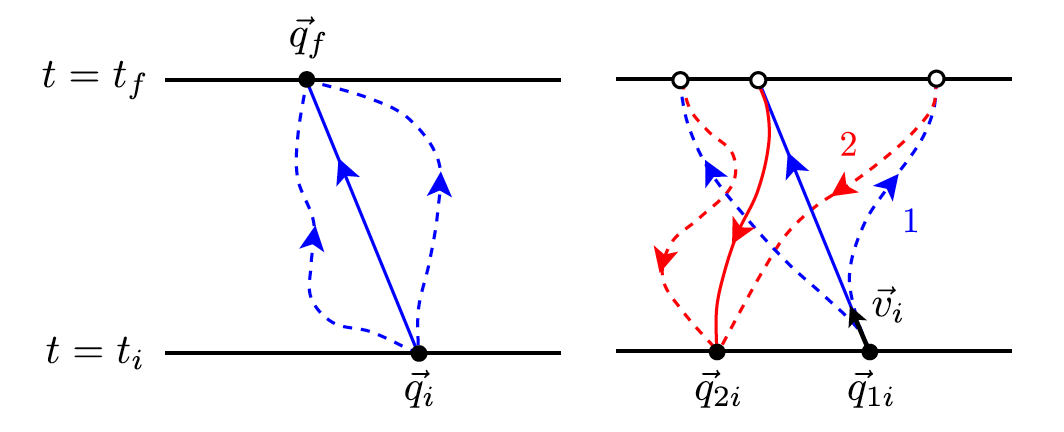
\includegraphics[width=0.7\textwidth,height=0.3\textwidth]{Galley.png}}
 \vspace{-0.5em}
 {\fontsize{9}{9}\caption{Hamilton's principle in VA \textcolor{darkgray}{(left)} versus NCVA \textcolor{darkgray}{(right)}.}}
 \vspace{-0.25em}
  { \tiny Source: \fullcite{Galley}\par}
\end{figure}
%\pause
\begin{columns}
\begin{column}{0.52\textwidth}
\fontsize{9}{9}\selectfont \begin{itemize} \item Introduce two sets of $N$ generalized coordinates and velocities, $\vec{q}_1$ and $\vec{q}_2$. 
\item Parametrize both coordinates: 
\begin{align}
\vec{q}_{1,2} (t, \epsilon) = \vec{q}_{1,2} (t, 0) + \epsilon \vec{\eta}_{1,2}(t). \nonumber
\end{align} 
\item $\vec{q}_{1,2} (t, 0)$ = stationary paths {\tiny $\epsilon \ll 1$  \textcolor{darkgray}{(solid lines)}}. 
\item $\vec{\eta}_{1,2}(t)$ = virtual displacements {\tiny \textcolor{darkgray}{(dashed lines)}}.
\end{itemize}
\end{column}
%\pause
\begin{column}{0.5\textwidth}
%\pause
Equality conditions for varying the action:
%\pause
\fontsize{9}{11}\selectfont  \begin{itemize}
\item $\vec{\eta}_{1,2}(t_i) = 0, $
\item $\vec{q}_{1} (t_f, \epsilon) = \vec{q}_{2} (t_f, \epsilon), $
\item $\dot{\vec{q}}_{1} (t_f, \epsilon) = \dot{\vec{q}}_{2} (t_f, \epsilon).$
\end{itemize}
%\pause
Equality does not fix values at final time. \\
%\pause 
After all variations, both paths are set equal and identified with physical limit.
\end{column}
\end{columns}
\end{frame}
% End Slide

% Slide 4
\begin{frame}[c]{Variational Theory of Non-conservative Systems}{Action functional}
\begin{block}{Definitions}
\begin{itemize}
\item \textcolor{paleblue}{Action functional} = Lagrangian + Non-conservative forces ($\mathcal{R}$):
\begin{align}
S[\vec{q}_n] &\equiv \int_{t_i}^{t_f} dt \; \left[\mathcal{L} (\vec{q}_1, \dot{\vec{q}}_1)  - \mathcal{L}(\vec{q}_2, \dot{\vec{q}}_2) + \mathcal{R} (\vec{q}_n, \dot{\vec{q}}_n, t) \right]. \nonumber 
\end{align}
\item Define \textcolor{paleblue}{new Lagrangian}:
\begin{align}
\Lambda (\vec{q}_n, \dot{\vec{q}}_n) \equiv  \mathcal{L} (\vec{q}_1, \dot{\vec{q}}_1) - \mathcal{L} (\vec{q}_2, \dot{\vec{q}}_2) + \mathcal{R} (\vec{q}_n, \dot{\vec{q}}_n, t). \nonumber
\end{align}
\end{itemize}
\end{block}
\end{frame}
% End Slide 

%Slide 5
\begin{frame}[c]{Variational Theory of Non-conservative Systems}{Change of Variables}
 \begin{itemize}
\item For \textcolor{paleblue}{convenience}: $\vec{q}_+ = (\vec{q}_1 +\vec{q}_2)/2$ and $\vec{q}_- = \vec{q}_1  -\vec{q}_2$. 
\item Physical limit:  \ALERT{$\vec{q}_- \rightarrow 0$} and \ALERT{$\vec{q}_+ \rightarrow \vec{q}$}.
\item New parametrized paths: $\vec{q}_{\pm} (t, \epsilon) = \vec{q}_{\pm} (t, 0) + \epsilon \vec{\eta}_{\pm}(t)$.
%\pause
\item For all $\vec{\eta}_{\pm}$ the action is stationary: \begin{align}(dS[\vec{q}_\pm]/d\epsilon)_{\epsilon = 0} = 0, \nonumber \end{align}
 given equality conditions are satisfied and \\
 $\vec{\eta}_- (t_f)   =  \vec{\eta}_\pm(t_i)  = 0$ $\rightarrow$ \ALERT{boundary terms vanish}.
\end{itemize}
\end{frame}
% End Slide


%Slide 6
\begin{frame}[c]{Variational Theory of Non-conservative Systems}{Non-conservative Euler-Lagrange Equations}
\begin{itemize}
\item In the physical limit ($\mathrm{PL}$), the action is stationary given that
\begin{align}
\Bigg[ \frac{\partial \Lambda}{\partial \vec{q}_-} \Bigg]_{\mathrm{PL}} = \frac{\partial \mathcal{L}}{\partial \vec{q}} + \Bigg[ \frac{\partial \mathcal{R} }{\partial \vec{q}_-}\Bigg]_{\mathrm{PL}}. \nonumber
\end{align}
\item The same can be shown for the conjugate momenta.
\item Equations of motion follow variational principle in $\mathrm{PL}$:
\begin{align}
\Bigg[\frac{ \delta S[\vec{q}_{\pm}] }{\delta \vec{q}_- (t)}\Bigg]_{\mathrm{PL}} = 0. \nonumber
\end{align}
\end{itemize}
\end{frame}
% End Slide

%Slide 7
\begin{frame}[c]{Non-conservative Variational Approximation}{NCVA Method for NLS}
\small{ 
\begin{itemize}
 \item Take the NLS: \[ i u_t + \frac{1}{2} u_{xx} + g |u|^2 u = \mathcal{P}. \]
%\pause
\item Lagrangian density for conservative NLS
\[ \mathcal{L} = \frac{i}{2} (u^* u_t - u u^*_t) + \frac{1}{2} |u_x|^2  - \frac{1}{2} g |u|^4. \]
\item Construct correct $\mathcal{R} = \mathcal{P}u_-^* + $ constant: 
\[
\mathcal{P} = \Bigg[ \frac{\partial \mathcal{R}}{\partial u_{-}^*}\Bigg]_{\mathrm{PL}}.  
\]
%\[
%u_1 = a_1\, \mathrm{sech}(w_1\,(x-\xi_1))e^{i(d_1 (x-\xi)^2 + c_1 (x-\xi_1)+b_1)},  \]
%\[u_2 = a_2 \, \mathrm{sech}(w_2\, (x-\xi_2))e^{i(d_2 (x-\xi)^2 + c_2 (x-\xi_2)+b_2)}. 
%\]
%\pause
\item NCVA Total Lagrangian with $\mathcal{L}_i \equiv \mathcal{L}(u_i, u_{i,t}, u_{i,x}, ..t)$ for $i=1,2$:   
\[ \mathcal{L}_T = \mathcal{L}_1- \mathcal{L}_2 + \mathcal{R}. \]
%\pause ~\footcustomcite{Kevrekidis2014}
%\pause 
\item Take your ans\"{a}tze:  $u_1$ and $u_2$.
\end{itemize}
}
%\end{block}
\end{frame}
% End Slide

%Slide 8
\begin{frame}[c]{Non-conservative Variational Approximation}{NCVA Method for NLS Continued}
%\frametitle[NCVA]{Non-Conservative Variational Approximation}
%\begin{columns}
%\begin{column}{0.5\textwidth}
%\begin{block} %{NCVA Method Continued}%~\cite{Kevrekidis2014}}
\small{
\begin{itemize}
\item  Integrate effective Lagrangian
\[ \bar{L} = \int \left(\bar{\mathcal{L}}_1 - \bar{\mathcal{L}}_2+ \bar{\mathcal{R}} \right)dx. \]
\item $\bar{\mathcal{L}}_1$ and $\bar{\mathcal{L}}_2$ recover same equations of motion as the conservative VA. 
%\small{Conserved terms:  Integrate, take derivative w.r.t $p_-$ at $\mathrm{PL}$, and recover conserved Euler-Lagrange equations of motion:}
%\tiny{\[ \int \left( \bar{\mathcal{L}}_1 - \bar{\mathcal{L}}_2\right) dx \rightarrow \; \Bigg[ \frac{\partial \bar{\mathcal{L} }}{\partial p_-} \Bigg]_{\mathrm{PL}} \; \mathrm{ \& } \; \; \; \; \Bigg[\frac{\partial \bar{\mathcal{L}} }{\partial \dot{p}_-} \Bigg]_{\mathrm{PL}}. \] }
%rightarrow \; \mathrm{Euler}\textrm{-}\mathrm{Lagrange }
%\pause
\item Non-conserved terms:  Take derivative w.r.t $p_-$ at $\mathrm{PL}$ then integrate: 
\[ \bar{R} = \int \Bigg[ \frac{\partial \bar{\mathcal{R}}}{\partial p_-} \Bigg]_{\mathrm{PL}} dx.   \] 
%\pause 
\item Put everything back together for \textcolor{paleblue}{modified Euler-Lagrange equations}:
\[ \frac{\partial \bar{L}}{\partial p} - \frac{d}{dt} \left( \frac{\partial \bar{L} }{\partial\dot{p}} \right) + \int  \Bigg[ \frac{\partial \bar{\mathcal{R}}}{\partial p_-} \Bigg]_{\mathrm{PL}} dx = 0. \]
\item Solve the system of equations!
\end{itemize} 
}
%\end{block}
\end{frame}
% End Slide

%Slide 9 : p-VA
\begin{frame}[c]{Perturbed Variational Approximation}{Perturbation Theory within VA}
%\frametitle[PVA]{Perturbed Variational Approximation}
%\begin{columns}
%\begin{column}{0.5\textwidth}
\begin{block}{ }
\fontsize{9}{9}\selectfont{
\begin{itemize}
\item Take NLS equation: $ i u_t + \frac{1}{2} u_{xx} + g|u|^2 u = 0. $
\item Perturb the equation $0 < \epsilon \ll 1$: \[ iu_t + \frac{1}{2} u_{xx} + |u|^2 u = \epsilon Q(u, u_x, u_t, ..., x, t) \]
\item Use ansatz:  $\bar{u}(x,t,\vec{p})$ %$ u = a\, \mathrm{sech}(w\, (x-\xi)) e^{i(d \, (x-\xi)^2 + c\,(x-\xi)+b)} $
\item Using $\mathcal{P} = \epsilon Q$, get $\mathcal{O}(\epsilon)$ perturbed Euler-Lagrange equations~\footcustomcite{KodamaAlbowitz1981}: %\footcustomcite{KodamaAlbowitz1981}: 
\[ \frac{\partial \bar{L}}{\partial p} - \frac{d}{dt}\frac{\partial \bar{L}}{\partial \dot{p}} =  \int \left( \bar{\mathcal{P}}^* \frac{\partial \bar{u}}{\partial p} + \bar{\mathcal{P}} \frac{\partial \bar{u}^*}{\partial p} \right) dx \equiv 2  \mathrm{Re} \int \bar{\mathcal{P}} \frac{\partial \bar{u}^*}{\partial p} dx \]
\end{itemize}
}
\end{block}
\end{frame}
% End Slide

%Slide 10
\begin{frame}[c]{Non-conservative VA = Perturbed VA}
Assume complex $\mathcal{P}$ to construct the functional $\mathcal{R}$ evaluated at the variational ansatz:
\[ \bar{\mathcal{P}} = \Bigg[ \frac{\partial \bar{\mathcal{R}}}{\partial \bar{u}_-^*} \Bigg]_{\mathrm{PL}} \]
Require real variational parameters such that
\[ \bar{\mathcal{R}} =\bar{\mathcal{P}} \left( \bar{u}_\pm, \bar{u}_\pm^*, \bar{u}_{\pm,t},\ldots \right) \bar{u}_-^*  +  \mathrm{complex \; \;  conjugate}. \]
Therefore, the PVA = NCVA
\[
\bar{P} = \int \bar{\mathcal{P}} dx =\int \Bigg[\frac{\partial \bar{\mathcal{R}}}{\partial p_-^* } \Bigg]_{\mathrm{PL}} dx \equiv \int \left(\bar{\mathcal{P}}^* \frac{\partial  \bar{u}}{\partial p^* } + \bar{\mathcal{P}} \frac{\partial  \bar{u}^*}{\partial p} \right)dx.  % \equiv 2 \mathrm{Re} \int Q \frac{\partial  u^*}{\partial p }dx. \nonumber
\]
%
%\end{itemize} 
%\end{block}
\end{frame}
%End Slide


%Slide 11: Linear Loss
\begin{frame}[c]{Non-conservative System}{NLS with Linear Loss}
\begin{center}
 \ALERT{$ i u_t + \frac{1}{2} u_{xx} + |u|^2 u = -i\epsilon u $}  \\
\end{center}
 
\COMMENT{Ansatz with $\vec{p} = (a, w, \xi, c, b, \phi)$:   
 \[ u_A (x,t;\vec{p}) = a\, \mathrm{sech}\left(w\, (x-\xi)\right) \exp\left[{i(b \, (x-\xi)^2 + c\,(x-\xi)+\phi)}\right] \]}  \\

\textcolor{darkgray}{\small{Lagrangian Density: $\bar{\mathcal{L}} =  \frac{i}{2} \left(\bar{u} \bar{u}_{t}^* - \bar{u}^* \bar{u}_{t} \right)  + \frac{1}{2} |\bar{u}_{x}|^2 - \frac{1}{2} |\bar{u}|^4$}}

\begin{columns}
\begin{column}{0.5\textwidth}
\begin{block}{NCVA }
\vspace{-1em}
\begin{align} 
 \bar{u}_1 =& u_A(x, t; \vec{p}_1), \nonumber \\
 \bar{u}_2 =& u_A(x, t; \vec{p}_2),  \nonumber \\
\bar{\mathcal{R}} =& i \epsilon u_+ u_-^* - i \epsilon u_+^*u_-, \nonumber \\
=&  i \epsilon (u_2u_1^* - u_1 u_2^* ),\nonumber \\
\mathcal{L}_T =& \mathcal{L}_1 - \mathcal{L}_2 + \mathcal{R}. \nonumber
% =& \frac{i}{2} \epsilon (u_1u_1^* - u_2 u_2^* + u_2u_1^* - u_1 u_2^*)  \nonumber \\
%&- \frac{i}{2} \epsilon (u_1u_1^* - u_2 u_2^* + u_2^*u_1 - u_1^* u_2), \nonumber\\
% =&   i \epsilon (u_2u_1^* - u_1 u_2^* ). \nonumber
 \end{align} 
\vspace{-1em}
\end{block}
\end{column}
\begin{column}{0.5\textwidth}
\begin{alertblock}{ODEs}
\vspace{-1em}
 \[ \begin{cases} 
 \dot{a} = - ab -  \epsilon a, \\ 
 \dot{b} = \frac{2w^4}{\pi^2} - \frac{2a^2 w^2}{\pi^2} - 2 b^2, \\
 \dot{c} = 0, \\ 
 \dot{d} = \frac{5}{6} a^2 + \frac{1}{2} c^2 - \frac{1}{3} w^2, \\
\dot{w} = -2bw, \\
 \dot{\xi} = c. \\ 
 \end{cases} \] 
\end{alertblock}
\end{column}
\end{columns}
\end{frame}
% End Slide

%Slide 12
\begin{frame}[c]{Numerical Results}{NLS with Linear Loss}
\begin{figure}[H!]
\centering
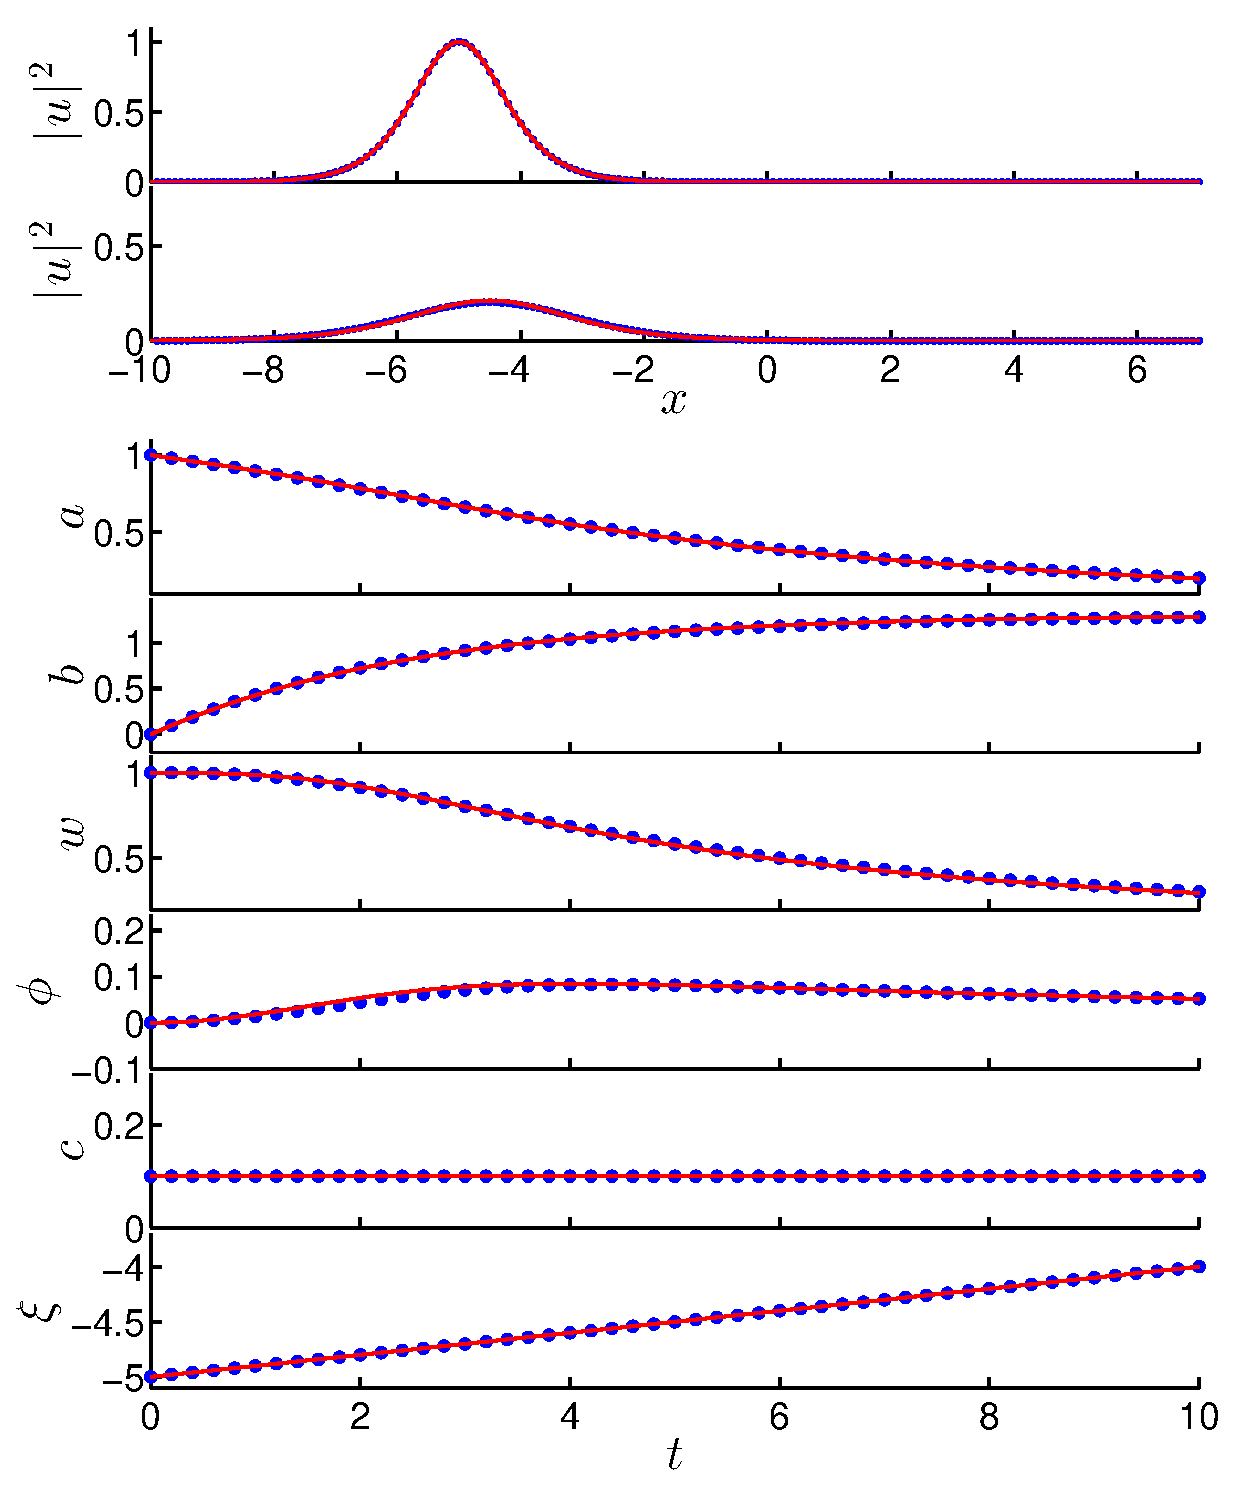
\includegraphics[height = 6cm,width = 5cm]{Fig1a_LL_e01N.eps} \quad
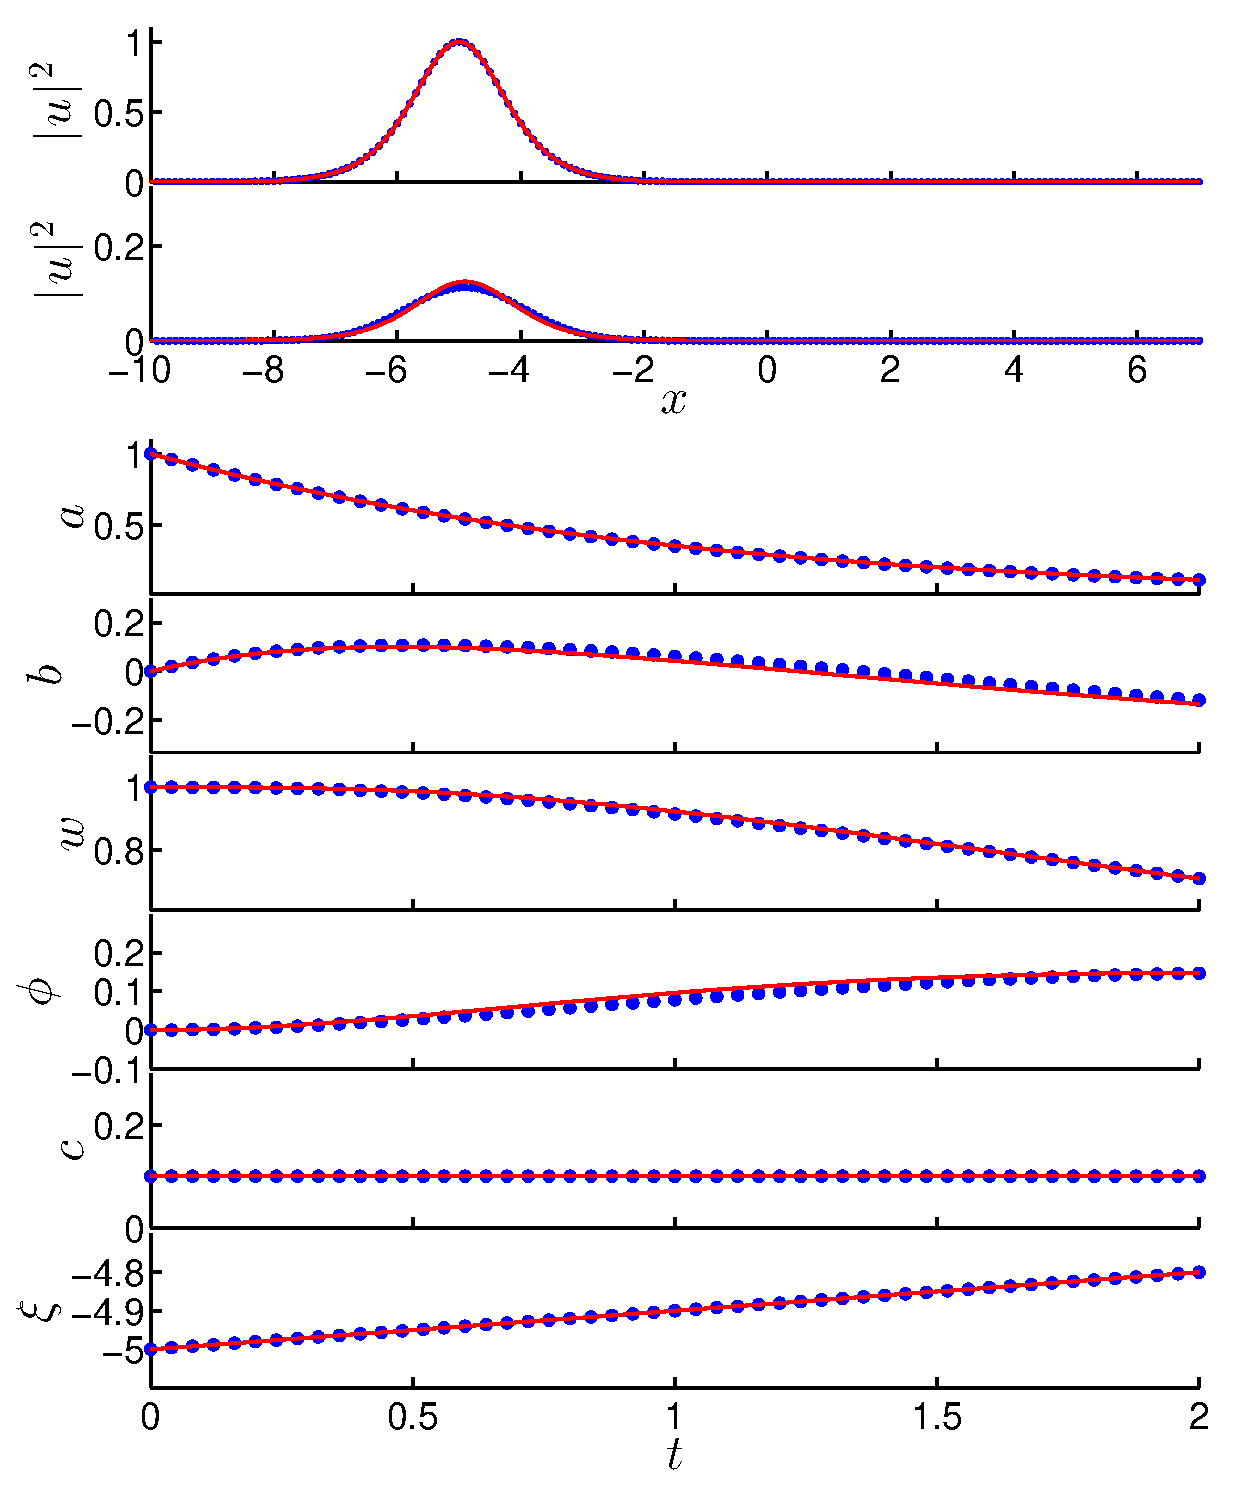
\includegraphics[height = 6cm,width = 5cm]{Fig1b_LL_e1N.eps}
%\vspace{-2em}
\caption{
Evolution of an NLS bright soliton solution under the presence of linear loss
of strength $\epsilon=0.1$ \textcolor{darkgray}{(left)} and $\epsilon=1$ \textcolor{darkgray}{(right)}.
}
%
\end{figure}
\end{frame} 
%



%Slide 13: Density Dependent Loss
\begin{frame}[c]{Non-conservative System}{NLS with Density Dependent Loss}
\begin{center}
 \ALERT{$ i u_t + \frac{1}{2} u_{xx} + |u|^2 u =-i\epsilon |u|^2 u$}  \\
\end{center}
 
\COMMENT{Ansatz with $\vec{p} = (a, w, \xi, c, b, \phi)$:     
\[u_A (x,t;\vec{p}) = a\, \mathrm{sech}\left(w\, (x-\xi)\right) \exp\left[{i(b \, (x-\xi)^2 + c\,(x-\xi)+\phi)}\right] \]}  
\textcolor{darkgray}{Non-conservative forces:  $\mathcal{R}  =  i\epsilon ( \bar{u}_+ \bar{u}_+^* \bar{u}_+\bar{u}_-^* -  \bar{u}_+ \bar{u}_+^* \bar{u}_-\bar{u}_+^*) $}
%\begin{block}{NCVA \hspace{5em} $i u_t + \frac{1}{2} u_{xx} + |u|^2 u = $}
%\end{block}
\begin{center}
\begin{columns}
\begin{column}{0.5\textwidth}
\begin{alertblock}{ODEs}
\vspace{-1em}
 \[ \begin{cases} 
 \dot{a} = - ab - a^3 \epsilon \Big( \frac{2 }{\pi^2} + \frac{2}{3} \Big), \\ 
 \dot{b} = \frac{2}{\pi^2} w^4 - \frac{2}{\pi^2} a^2 w^2 - 2 b^2, \\
 \dot{c} = 0, \\ 
 \dot{d} = \frac{5}{6} a^2 + \frac{1}{2} c^2 - \frac{1}{3} w^2, \\
\dot{w} = -2bw - \frac{4}{\pi^2} \epsilon a^2 w , \\
 \dot{\xi} = c. \\ 
 \end{cases} \] 
\end{alertblock}
\end{column}
\end{columns}
\end{center}
\end{frame}

%Slide14: Density Dependent Loss Results
\begin{frame}[c]{Numerical Results}{NLS with Density Dependent Loss}
\begin{figure}[H!]
\centering
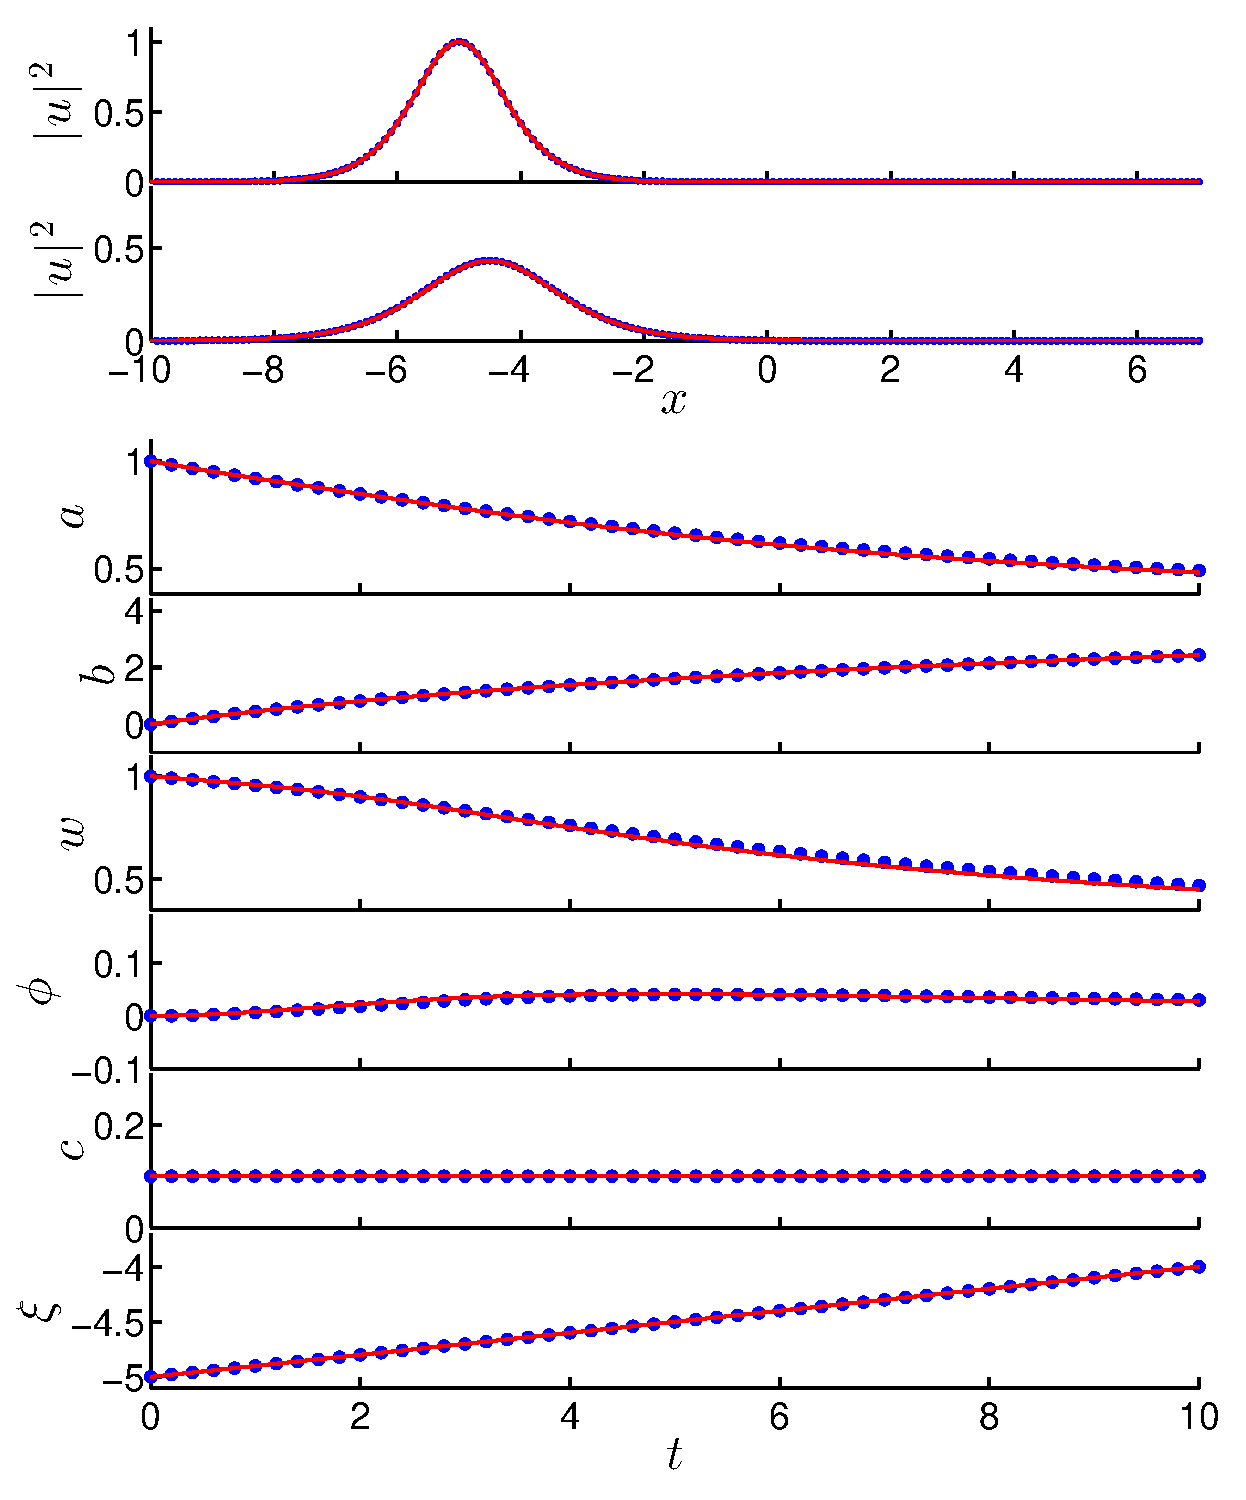
\includegraphics[height = 6cm,width = 5cm]{Fig2_DD_e01N.eps}
%\vspace{-2em}
\caption{
Evolution of an NLS bright soliton solution under the presence of density dependent loss
of strength $\epsilon=0.1$.
}
%
\end{figure}

\end{frame} 

%Slide 15: Polariton 
\begin{frame}[c]{Non-conservative System}{Exciton-Polariton Condensate}
%\frametitle{Dynamical System III:  Exciton-Polariton Condensate}
%\tikzstyle{na} = [baseline=-.5ex]

%\begin{itemize}[<+-| alert@+>]
  %  \item NLS
   %   \tikz[baseline=-.5ex]\node[fill=Alert,anchor=base, rounded corners] (numbnote) {};
   \tikz[baseline=-.5ex]\node[fill=Comment,anchor=north, rounded corners] (nlsnote) {
	\textcolor{white}{NLS}
	};  
  \hspace{4cm}\tikz[baseline=-.5ex]\node[fill=crimsonred,anchor=north, rounded corners] (gnote) {
	\textcolor{white}{Exciton Pumping:  Linear Gain }
	};

\vspace{1.5em}

\begin{align*}
        \tikz[baseline=-.5ex]{
            \node (nls) {\textcolor{Comment}%[fill=blue!20,anchor=base] (t1)
            {$ i u_t + \frac{1}{2} u_{xx} - |u|^2 u -V(x) u$}};
        } = i \left(
        \tikz[baseline=-.5ex]{
            \node (gain) {\textcolor{crimsonred}
            {$ \chi (x) u$}} ;
        }  -
        \tikz[baseline=-.5ex]{
	\node (loss) {\textcolor{paleblue}
            {$\sigma |u|^2 u$}};
        }
        \right).
\end{align*}

\vspace{ 1.5em}
	
	\hspace{6cm}\tikz[baseline=-.5ex]\node[fill=paleblue,anchor=north, rounded corners] (lossnote) {
	\textcolor{white}{Decay of Polaritons:  Density Dependent Loss}
	};

%\begin{itemize}[<+-| alert@+>]

  %  \item Decay of Polaritons:  Density Dependent Loss
    %    \tikz[na]\node [coordinate] (n2) {};
   % \item Exciton Pumping:  Linear Gain 
     %   \tikz[na]\node [coordinate] (n3) {};
%\end{itemize}

%\begin{tikzpicture}[overlay]
     %   \path[->]<1-> (n1) edge [bend left] (t1);
       % \path[->]<2-> (n2) edge [bend right] (t2);
        %\path[->]<3-> (n3) edge [out=0, in=-90] (t3);
   	\begin{tikzpicture}[overlay, line width=1.5]
	        \path[->,color=Comment] (nlsnote) edge [bend left] (nls);
	        	\path[->,color=crimsonred] (gnote) edge [bend right] (gain);
		\path[->,color=paleblue] (lossnote) edge [out=90, in=245] (loss);
	        % \path[->]<2-> (n2) edge [bend right] (t2);
	        % \path[->]<3-> (n3) edge [out=0, in=-90] (t3);
	\end{tikzpicture}

	\begin{center}	\textcolor{Comment}{$  V(x) = \frac{1}{2} \Omega^2 x^2 $ } \quad \quad  \quad 
	\textcolor{crimsonred}{$ \chi(x) =  \alpha \exp \left[ -\frac{x^2}{2\beta^2} \right] $}
	\end{center}

	
\end{frame}
%




%Slide16: Polariton 
\begin{frame}[c]{Numerical Results}{Exciton-Polariton Condensate}
%\tiny{	\[ \chi(x) = \alpha \exp\left(  -\frac{x^2}{2\beta^2} \right) \] 	
%	\[ V(x) = \frac{1}{2}\Omega^2 x^2 \] %
%	\[ u_A(x,t; \vec{p}) = a \exp \left( \frac{-x^2}{2 w^2}\right)  \exp \left( i \left(bx^2 + \phi\right)\right) \] }
%\vspace{-3em}
\begin{figure}[H!]
\centering
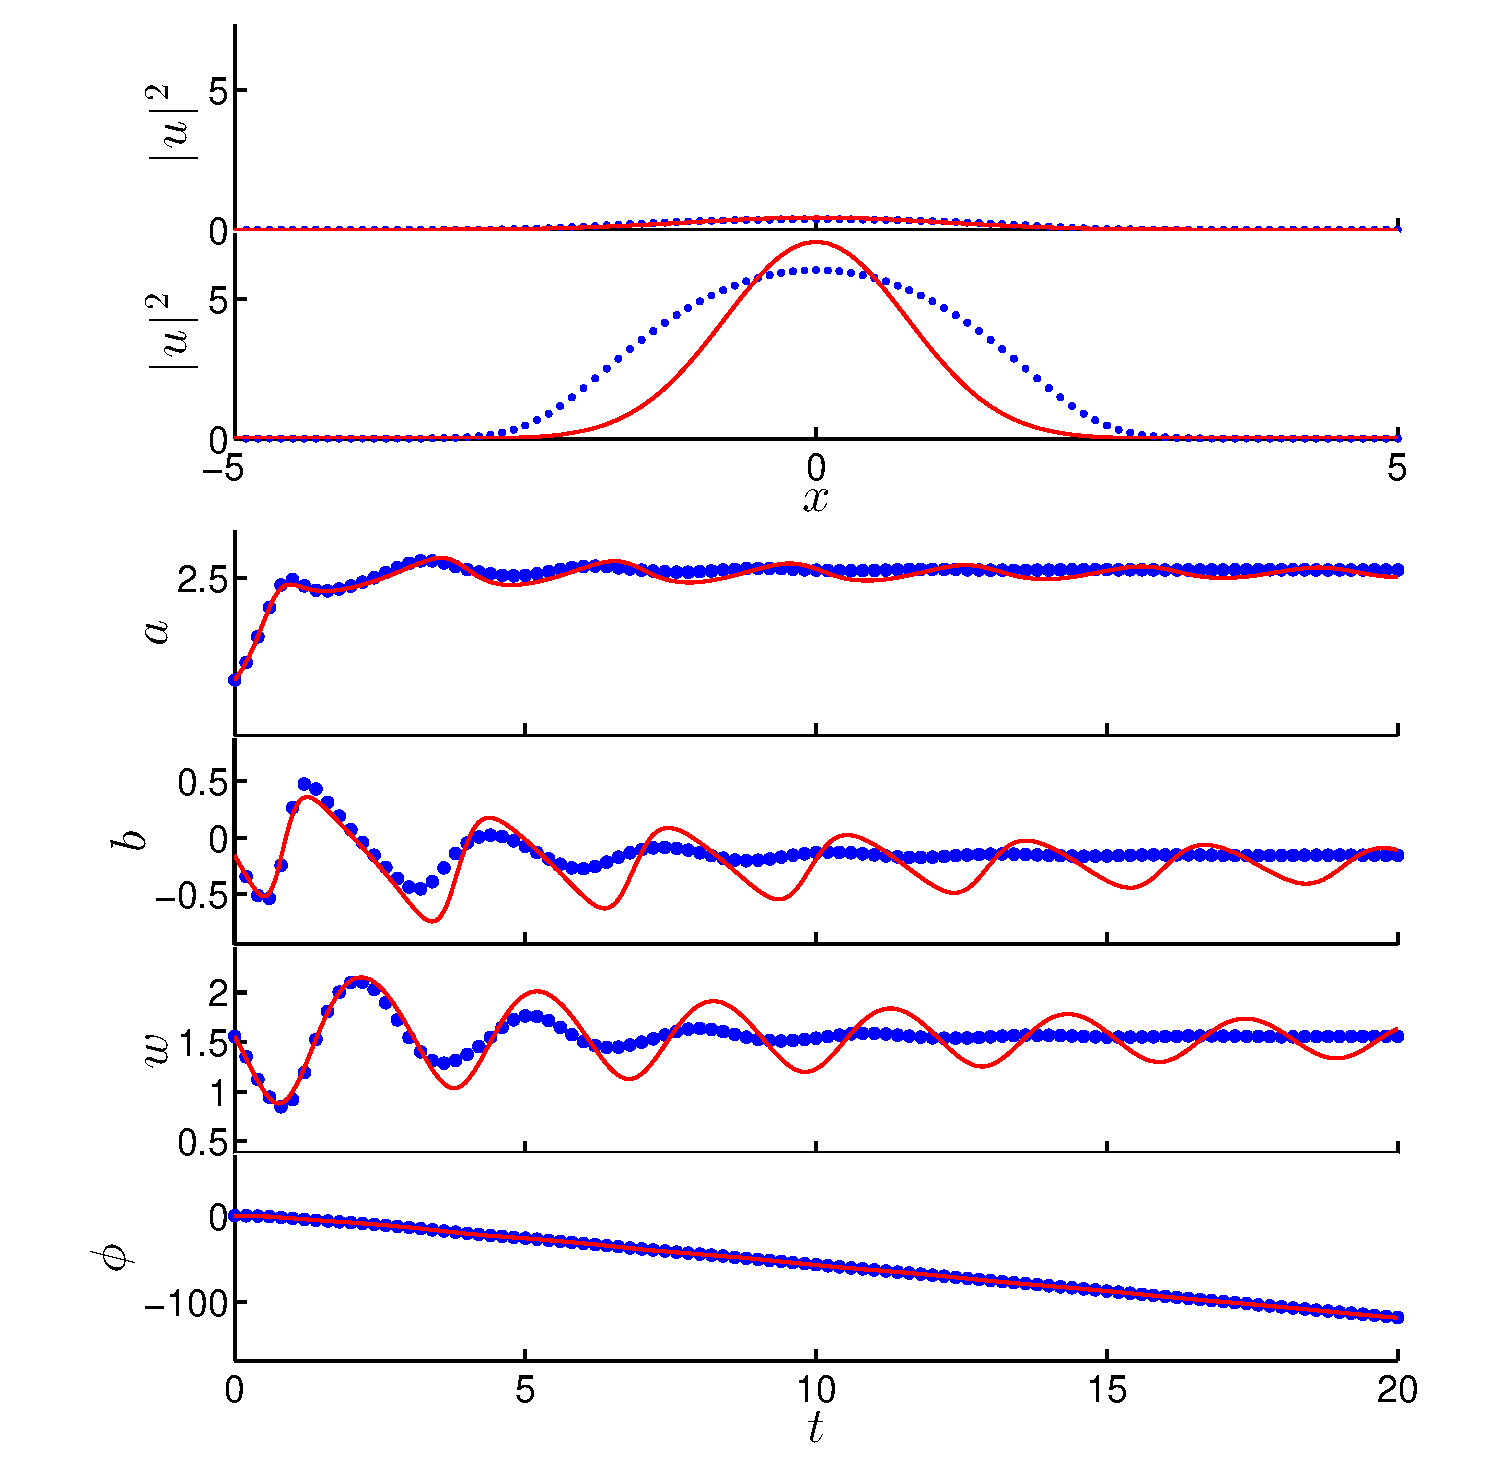
\includegraphics[height = 6cm, width = 5cm]{Fig3a_P4_increase_v2.eps}
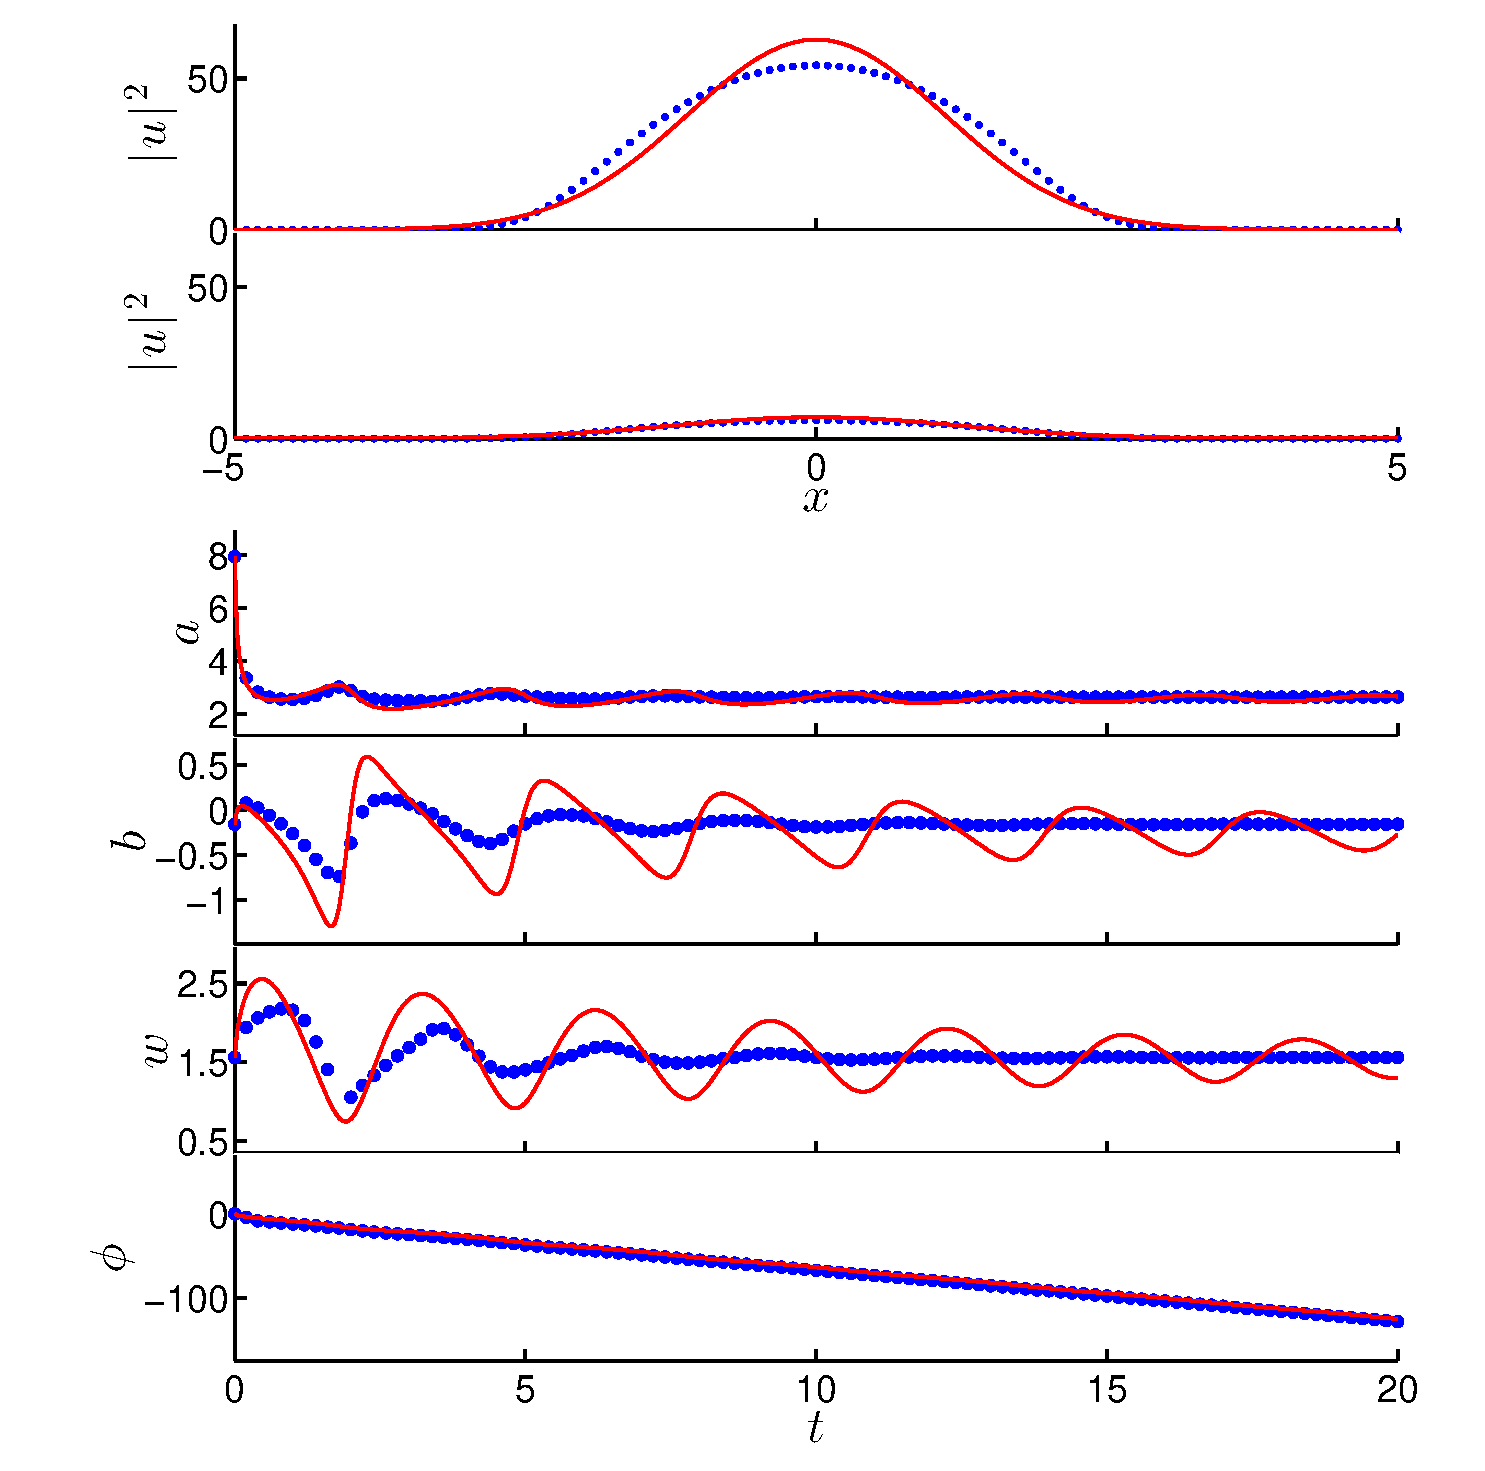
\includegraphics[height = 6cm, width = 5cm]{Fig3b_P4_decrease_v2N.eps}
\caption{\tiny{
Evolution of the trapped wavefunction with ansatz \textcolor{regal}{$u_A(x,t; \vec{p}) = a \exp \left( \frac{-x^2}{2 w^2}\right)  \exp \left( i \left(bx^2 + \phi\right)\right) $}
in the presence of a linear spatially
dependent gain $\chi(x) = \alpha \exp\left(  -\frac{x^2}{2\beta^2} \right)$ with
%$\chi(x)= \alpha \exp \left(-\frac{x^2}{2\beta^2}\right)$ with 
$\alpha =2$ and $\beta=2$ and density dependent loss of strength 
$\sigma =0.37$, as well as a harmonic potential $V(x) = \frac{1}{2}\Omega^2 x^2$
of strength $\Omega = \sqrt{2}$.}}
\end{figure}
\end{frame}

%\begin{frame}[c]{Numerical Results}{Exciton-Polariton Condensate: Dynamics}
%\vspace{-3em}
%\begin{figure}[H!]
%\centering
%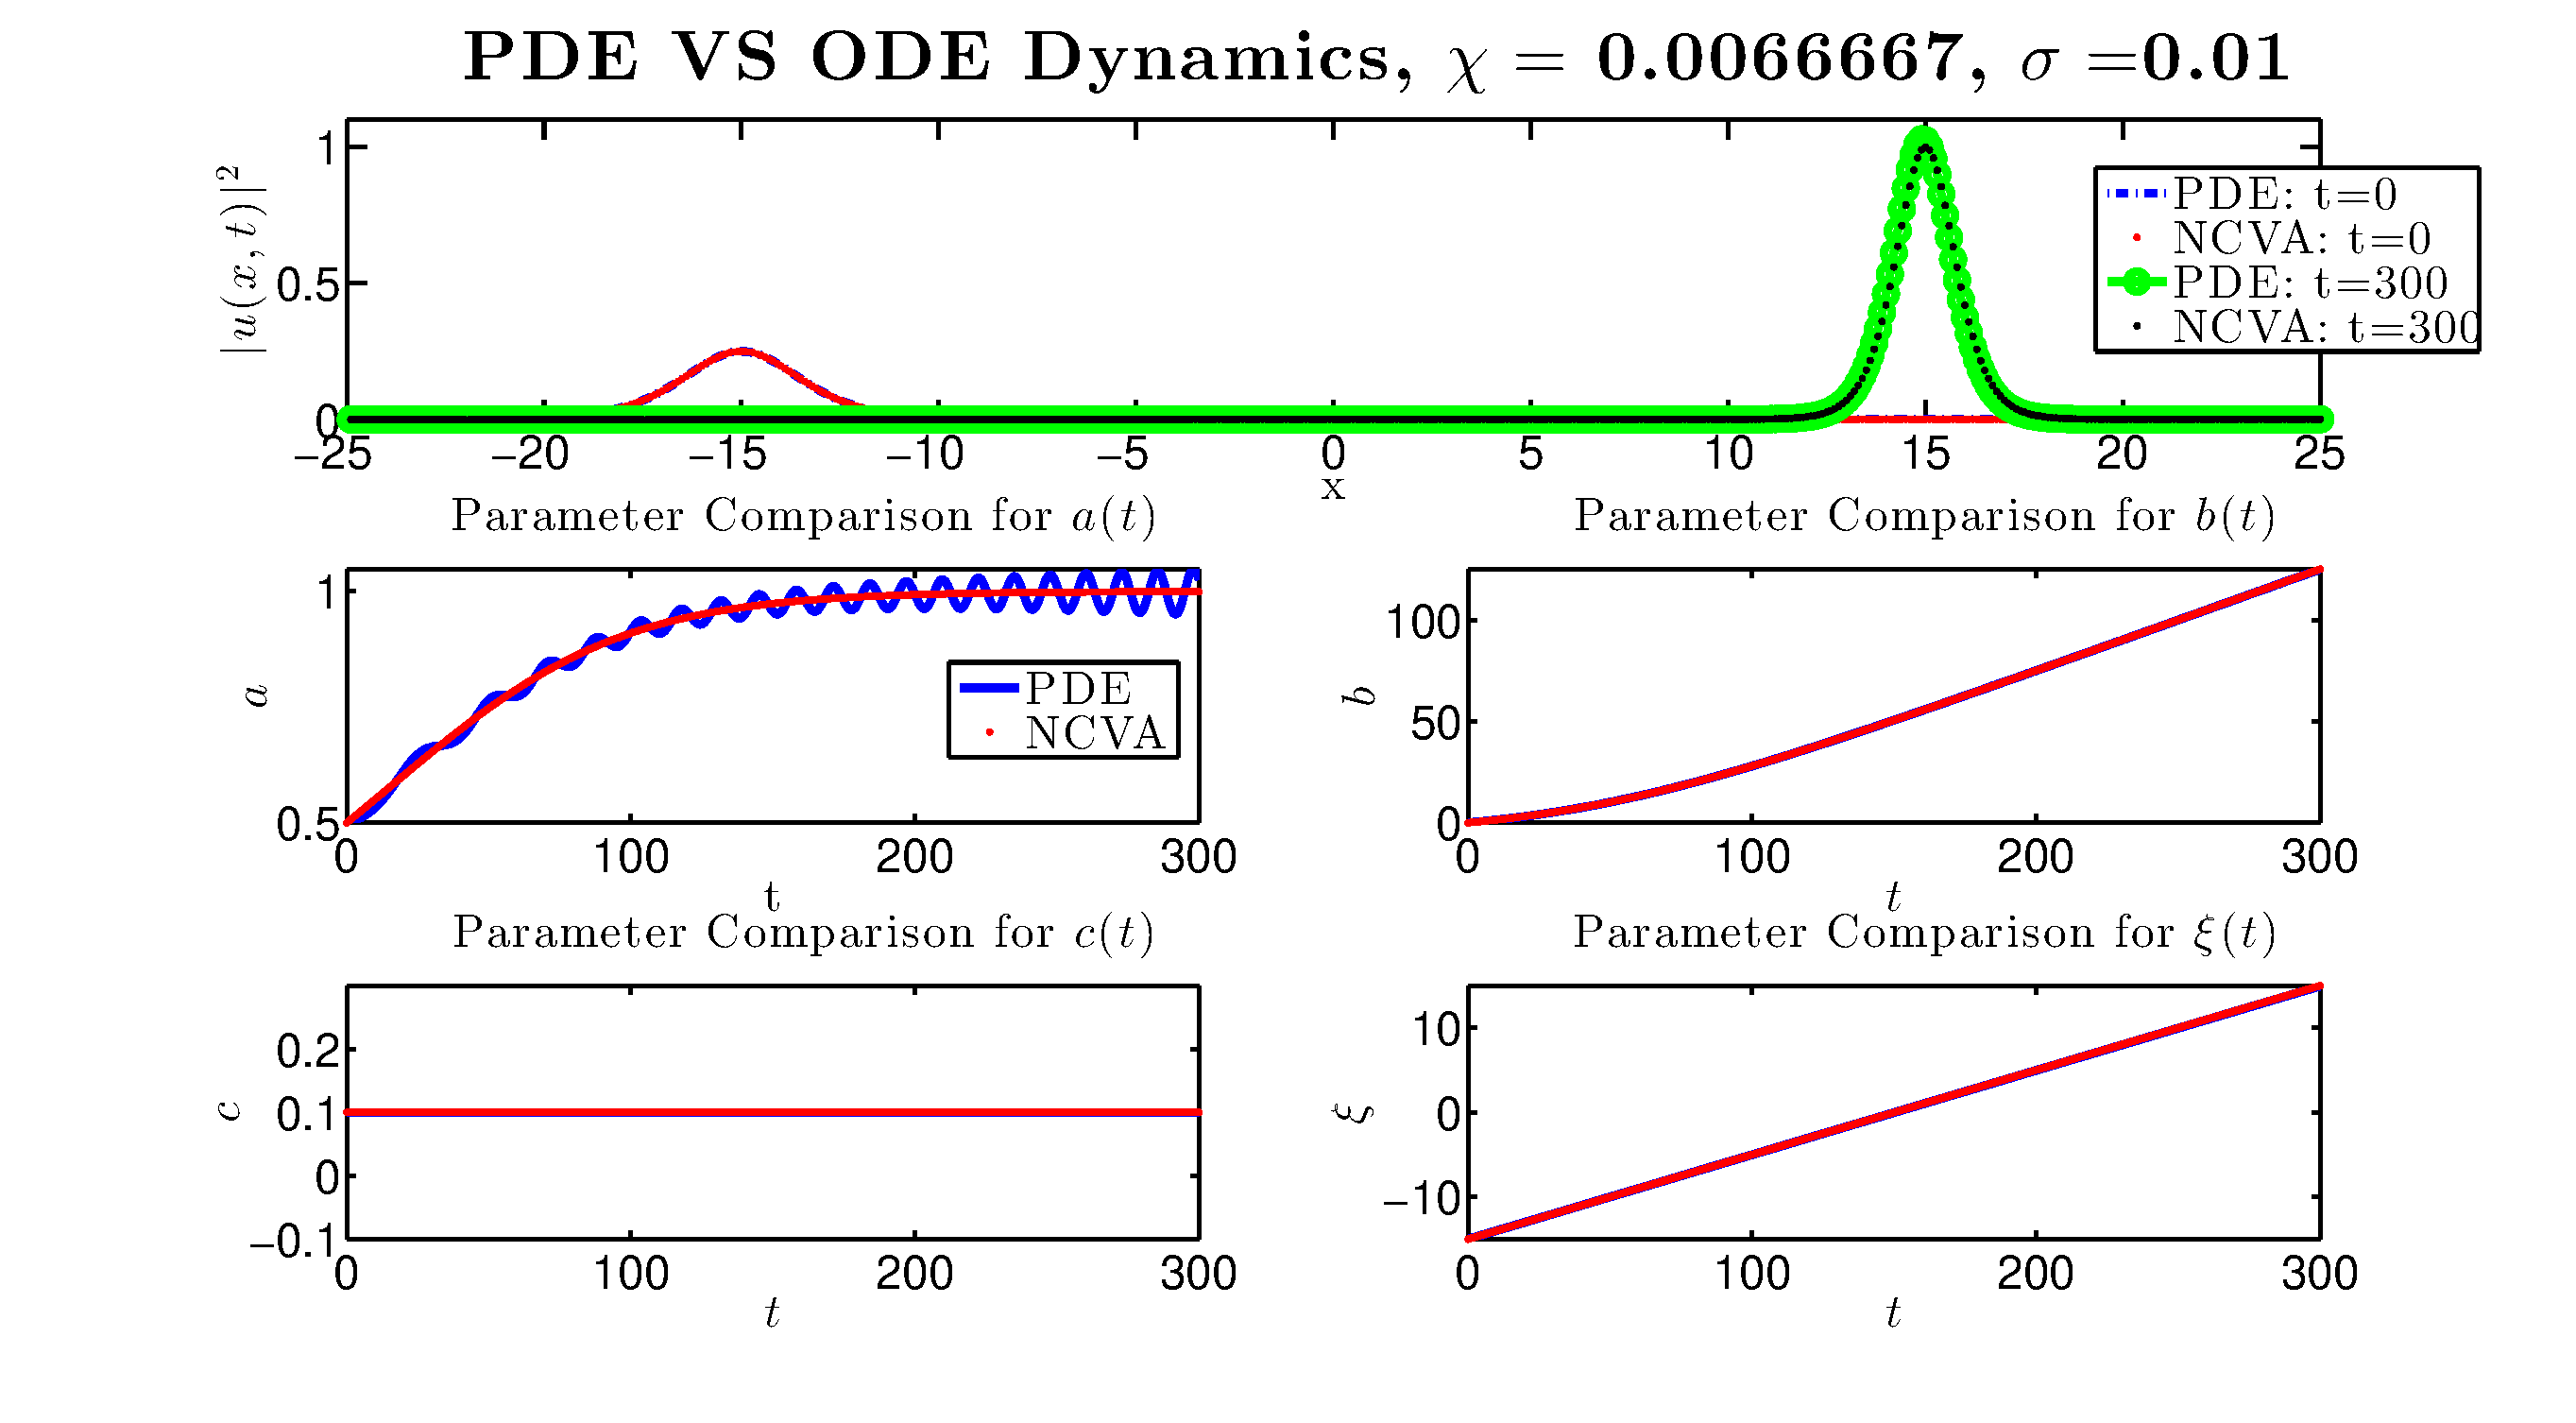
\includegraphics[height = 11cm, width = 10cm, angle = 90]{Pcase4}
%\end{figure}
%\end{frame}


%\begin{frame}[c]{Non-conservative Variational Applications}{ $\mathcal{PT}$-symmetric sG and $\phi^4$}
%   \tikz[baseline=-.5ex]\node[fill=Comment,anchor=north, rounded corners] (kg_note) {
%	\textcolor{white}{Klein-Gordon}
%	};  
%\vspace{1em}
%
%\begin{align*}
%        \tikz[baseline=-.5ex]{
%            \node (kg) {\textcolor{Comment}%[fill=blue!20,anchor=base] (t1)
%            {$ u_{tt} - u_{xx}  $}};
%        } +
%        \tikz[baseline=-.5ex]{
%            \node (vu) {\textcolor{crimsonred}
%            {$V'(u) $}};
%        }  =
%        \tikz[baseline=-.5ex]{
%	\node (ncterm) {\textcolor{paleblue}
%            {$\gamma(x) u_t$ }} ;
%        }
%\end{align*}
%%\vspace{ 1em}
%
%	\tikz[baseline=-.5ex]\node[fill=crimsonred,anchor=north, rounded corners] (v_note){
%	\textcolor{white}{ sG: $V(u) = 1 - \cos(u)$ \quad $\mathbf{\phi^4}$: $V(u) = (u^2 - 1)^2/2$ }
%	};\\
%	\hspace{6em}\tikz[baseline=-.5ex]\node[fill=paleblue,anchor=north, rounded corners] (nc_note) {
%	\textcolor{white}{Loss/Gain:  $\gamma(u) = \epsilon \mathrm{tanh}(x) \mathrm{sech}(x)$}
%	};
%   	\begin{tikzpicture}[overlay, line width=1.5]
%	        \path[->,color=Comment] (kg_note) edge [bend left] (kg);
%	        	\path[->,color=crimsonred] (v_note) edge [bend right] (vu);
%		\path[->,color=paleblue] (nc_note) edge [out=0, in=0] (ncterm);
%	        % \path[->]<2-> (n2) edge [nc right] (t2);
%	        % \path[->]<3-> (n3) edge [out=0, in=-90] (t3);
%	\end{tikzpicture}
%	
%
%\end{frame}
%
%\begin{frame}[c]{Applications}{ $\mathcal{PT}$-symmetric sG and $\phi^4$}
%\begin{itemize}
%\item \small{ \fullcite{Kevrekidis2014}}
%\item \textcolor{paleblue}{Conservative} Lagrangian density
%\[ \mathcal{L} = \frac{u_t^2}{2} - \Big(\frac{u_x^2}{2} + V(u) \Big). \]
%\item Choose  \[ \mathcal{R} = \gamma(x) u_-u_{+,t}. \]
%\item Construct \[ \Bigg[\frac{\partial \mathcal{R}}{\partial u_-} \Bigg]_{PL} = \gamma(x)u_t \]
%\end{itemize}
%\end{frame}
%
%%\begin{frame}[c]{Applications}{ $\mathcal{PT}$-symmetric sG and $\phi^4$}
%%The conservative Lagrangian density
%%\[ L = \frac{u_t^2}{2} - \Big(\frac{u_x^2}{2} + V(u) \Big). \]
%%Construct \[ \Big[\frac{\partial R}{du_-} \Big]_{PL} = \gamma(x)u_t \]
%%by choosing 
%%\[ R = \gamma(x) u_-u_{+,x}. \]
%%Use ansatz \[ u_i = K[x - X_i(t)]\] for $i=1,2$
%%non-Hamiltonian equation of motion:
%%\[ M \ddot{X} = \dot{X} \int \gamma (x) [K'(x-X)]^2 dx \]
%%Dynamics of the kink solution and eigenvalues of the spectrum  
%%\end{frame}
%
%\begin{frame}[c]{Applications}{ $\mathcal{PT}$-symmetric sG}
% \small{ Ansatz for $i=1,2$ where $K(x-X_0) = 4 \mathrm{arctan} (e^{x-X_0})$: \[ \bar{u}_i = K[x - X_i(t)].\] 
%Non-Hamiltonian equation of motion:
%\[ M \ddot{X} = \dot{X} \int \gamma (x) [K'(x-X)]^2 dx. \]}
%\vspace{-1em}
%\begin{figure}[H!]
%\centering
%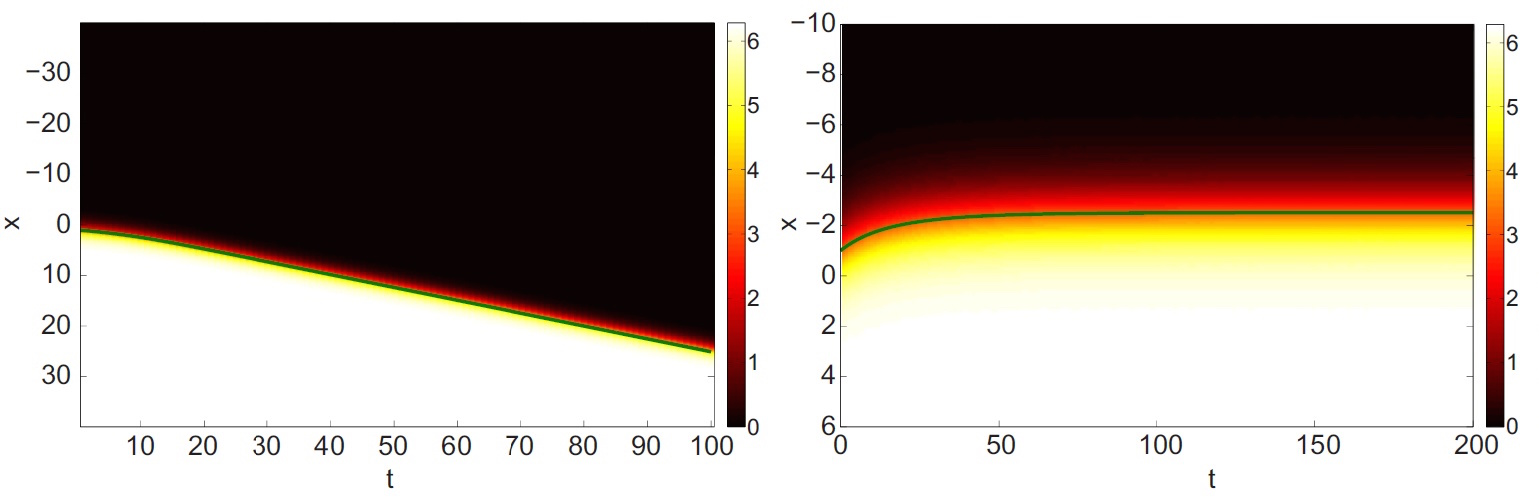
\includegraphics[width = \textwidth]{panos1.jpg}\caption{\tiny{~\fullcite{Kevrekidis2014}}}
%\end{figure}
%\end{frame}
%%
%%\begin{frame}[c]{Applications}{ $\mathcal{PT}$-symmetric  $\phi^4$}
%%Ansatz \[ u(x,t) = K[x - X_0(t)] + A(t) S[x-X_0(t)]\] 
%%Non-Hamiltonian equation of motion:
%%\begin{align*} M \ddot{X} = \dot{X} \int \gamma (x) [K'(x-X)]^2 dx, \\
%%\ddot{A} = -\omega^2 A + \dot{A} \int \gamma(x) S(x-X)^2 dx.
%% \end{align*}
%% \vspace{-1em}
%%\begin{figure}[H!]
%%\centering
%%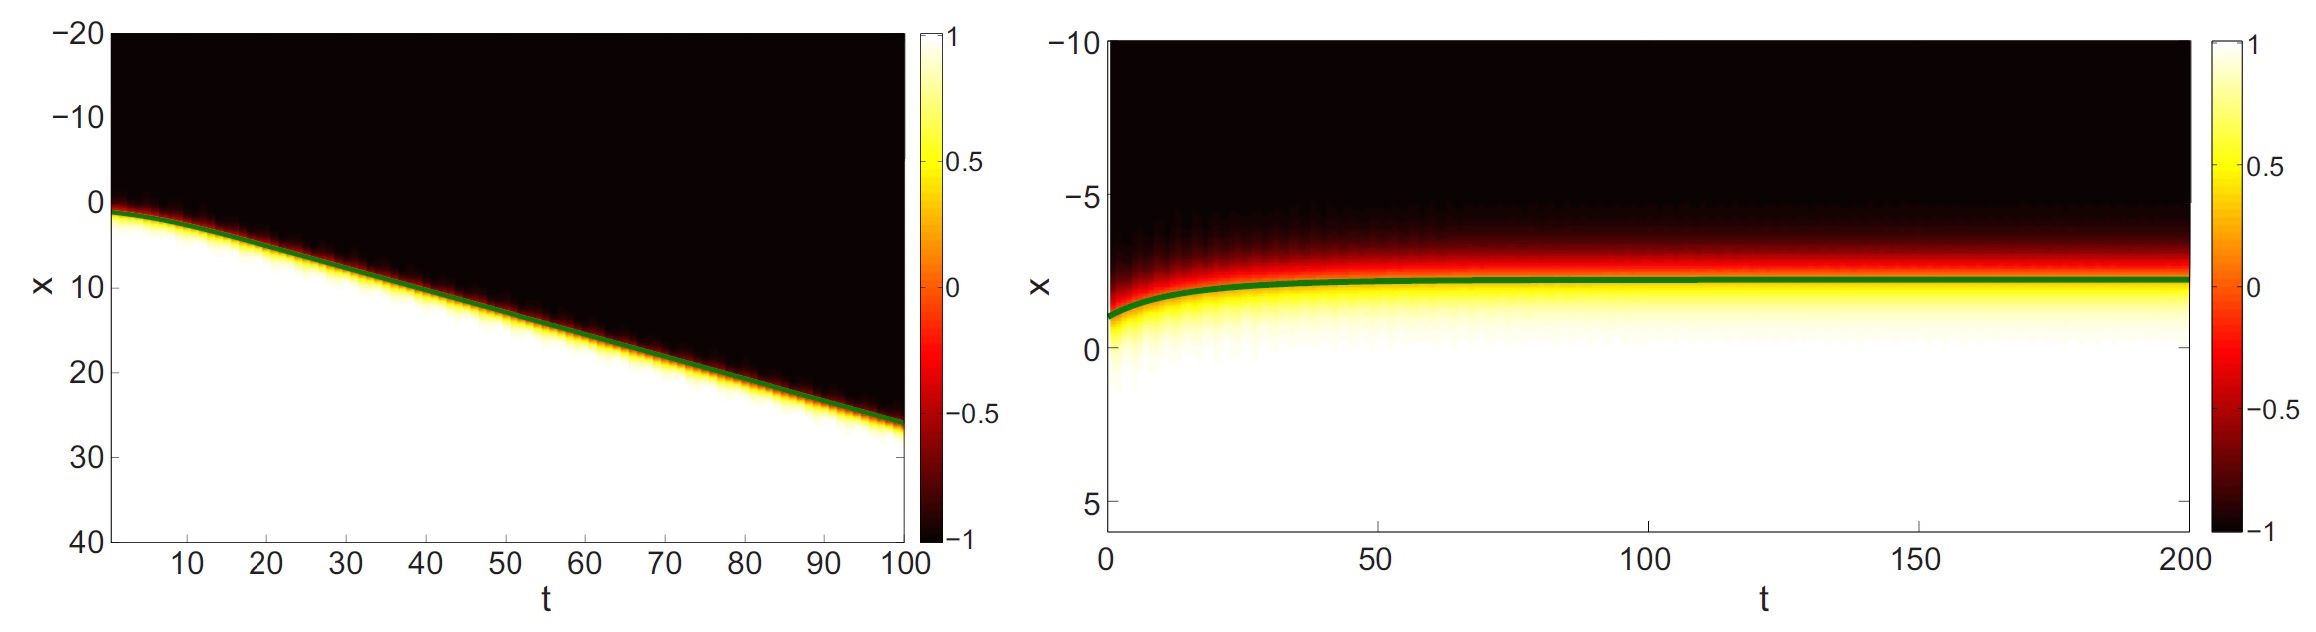
\includegraphics[width=8cm,height=2cm]{panos2.jpg}\caption{\tiny{~\fullcite{Kevrekidis2014}}}
%%\end{figure}
%%\end{frame}
%

%Slide 18
\begin{frame}[c]{Applications: Spontaneous Symmetry Breaking}{SSB in Passive Kerr Resonator}
%\vspace{-1em}
\begin{figure}[H!]
\centering
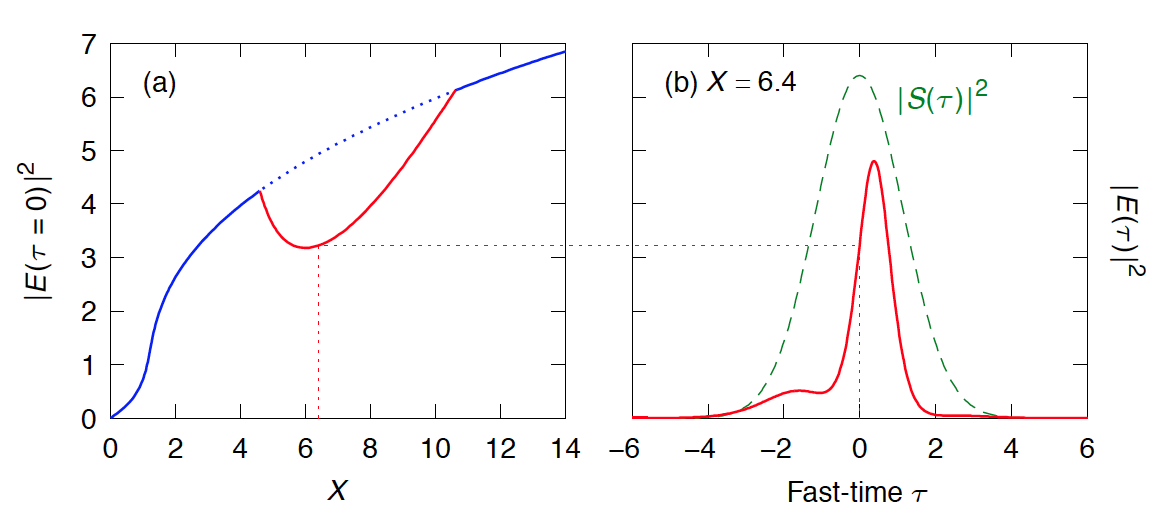
\includegraphics[height= 3.5cm]{XuCoenv2.png} \\
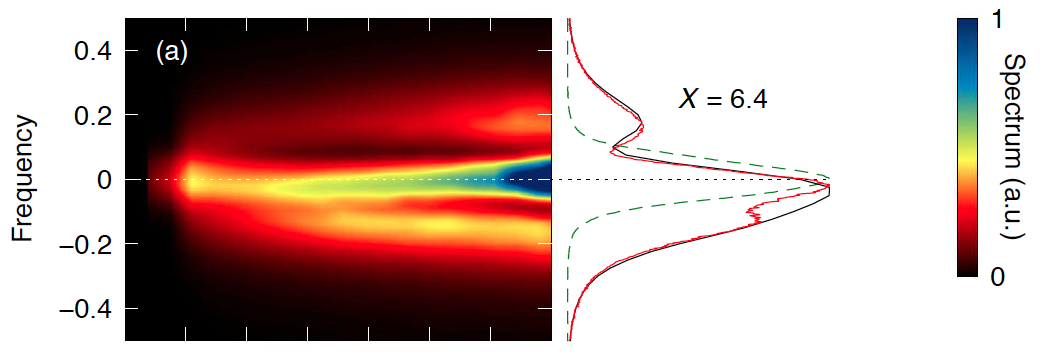
\includegraphics[ height = 2.5cm]{XuCoen2v2.png}
\vspace{-1em}
\caption{SSB Bifurcation Diagram and Experimental Output }
\tiny{Source:~\fullcite{XuCoen}}
\end{figure}
\end{frame}

%Slide 19
\begin{frame}[c]{Applications: SSB}{NLS with Cavity Boundary Conditions (Lugiato-Lefever Equation) }
   \tikz[baseline=-.5ex]\node[fill=Comment,anchor=north, rounded corners] (nlsnote2) {
	\textcolor{white}{NLS}
	};   \quad \quad 
	\hspace{2em}\tikz[baseline=-.5ex]\node[fill=turtlegreen,anchor=north, rounded corners] (phasenote) {
	\textcolor{white}{Cavity phase detuning ($\Delta = 0.92$) }
	};

\vspace{1.5em}

%\end{itemize}
\begin{align*}
        \tikz[baseline=-.5ex]{
            \node (nls) {\textcolor{Comment}%[fill=blue!20,anchor=base] (t1)
            {$ i u_z +  u_{\tau\tau} + |u|^2 u $}};
        }  -
        \tikz[baseline=-.5ex]{
	\node (phase) {\textcolor{turtlegreen}
            {$\Delta u$}};
        } =  -
        \tikz[baseline=-.5ex]{
            \node (lossi) {\textcolor{paleblue}
            {$ i u$}} ;
        } +
         \tikz[baseline=-.5ex]{
	\node (gainS) {\textcolor{crimsonred}
            {$i S(\tau)$}};
        }.
\end{align*}

\vspace{1.5em}
	
	\hspace{4em}\tikz[baseline=-.5ex]\node[fill=paleblue,anchor=north, rounded corners] (lossinote) {
	\textcolor{white}{Cavity losses}
	}; \quad  \quad  \quad \quad  
	\hspace{2em}\tikz[baseline=-.5ex]\node[fill=crimsonred,anchor=north, rounded corners] (gainSnote) {
	\textcolor{white}{External pumping ($T_0 = 2.3$)}
	};

   	\begin{tikzpicture}[overlay, line width=1.5]
	        \path[->,color=Comment] (nlsnote2) edge [bend left] (nls);
	        \path[->,color=turtlegreen] (phasenote) edge [bend left] (phase);
	        	\path[->,color=paleblue] (lossinote) edge [bend right] (lossi);
		\path[->,color=crimsonred] (gainSnote) edge [out=0, in=245] (gainS);
	        % \path[->]<2-> (n2) edge [bend right] (t2);
	        % \path[->]<3-> (n3) edge [out=0, in=-90] (t3);
	\end{tikzpicture}
	
	\textcolor{crimsonred}{\begin{align*} S(\tau) = \sqrt{X} \exp[-(\tau/T_0)^2 ]\end{align*}}

\end{frame}


%Slide 20
\begin{frame}[c]{Applications: SSB}{Equilibria, Stability and Bifurcations }
\small{\begin{itemize}
\item Identify stationary solutions $u(z,\tau) = u_0 (\tau)$ by solving steady-state equation:
\[ u_{0,\tau\tau} + \left( |u_0|^2 - \Delta \right) u_0 = -i u_0 + i S(\tau). \] 
\item Spectral stability analysis with small perturbations $\mathcal{O} (\epsilon)$:
\[ u(z,\tau) = u_0(\tau) + \epsilon \left[ a(\tau) e^{\lambda z} + b^*(\tau) e^{\lambda^* z} \right]. \]
\item Eigenvalue problem (eigenvalues $\lambda$, eigenvector $\xi = (a(\tau), b(\tau))^{\mathrm{T}}$): 
\small{\begin{align*}
i \lambda \begin{pmatrix}  a \\ b \end{pmatrix} = \begin{pmatrix} -\partial_{\tau}^2 - 2|u_0|^2 + (\Delta - i) & -u_0^2 \\ u_0^2 & \partial_{\tau}^2 + 2|u_0|^2 - (\Delta + i) \end{pmatrix}  \begin{pmatrix} a\\ b\end{pmatrix}.
\end{align*}}
\item \textcolor{paleblue}{Linearly} \ALERT{unstable} \textcolor{paleblue}{provided $\mathrm{Re}(\lambda)>0$}.
\end{itemize}}
\end{frame}


%Slide 21
\begin{frame}[c]{Applications: SSB}{Linearization Spectrum}
\begin{columns}
\begin{column}{0.5\textwidth}
\centering
         \includemedia[%
         	%label=freq,%
 		width=0.9\linewidth,%
  		%height=0.4\linewidth,%
		transparent=true,%
  		activate=onclick,%
		%deactivate=pageclose,%
		%stepping=true,%
  		addresource=EigMovieDefense.mp4,%
  		flashvars={source=EigMovieDefense.mp4 &loop=true &controlBarAutoHide=true}%
		]{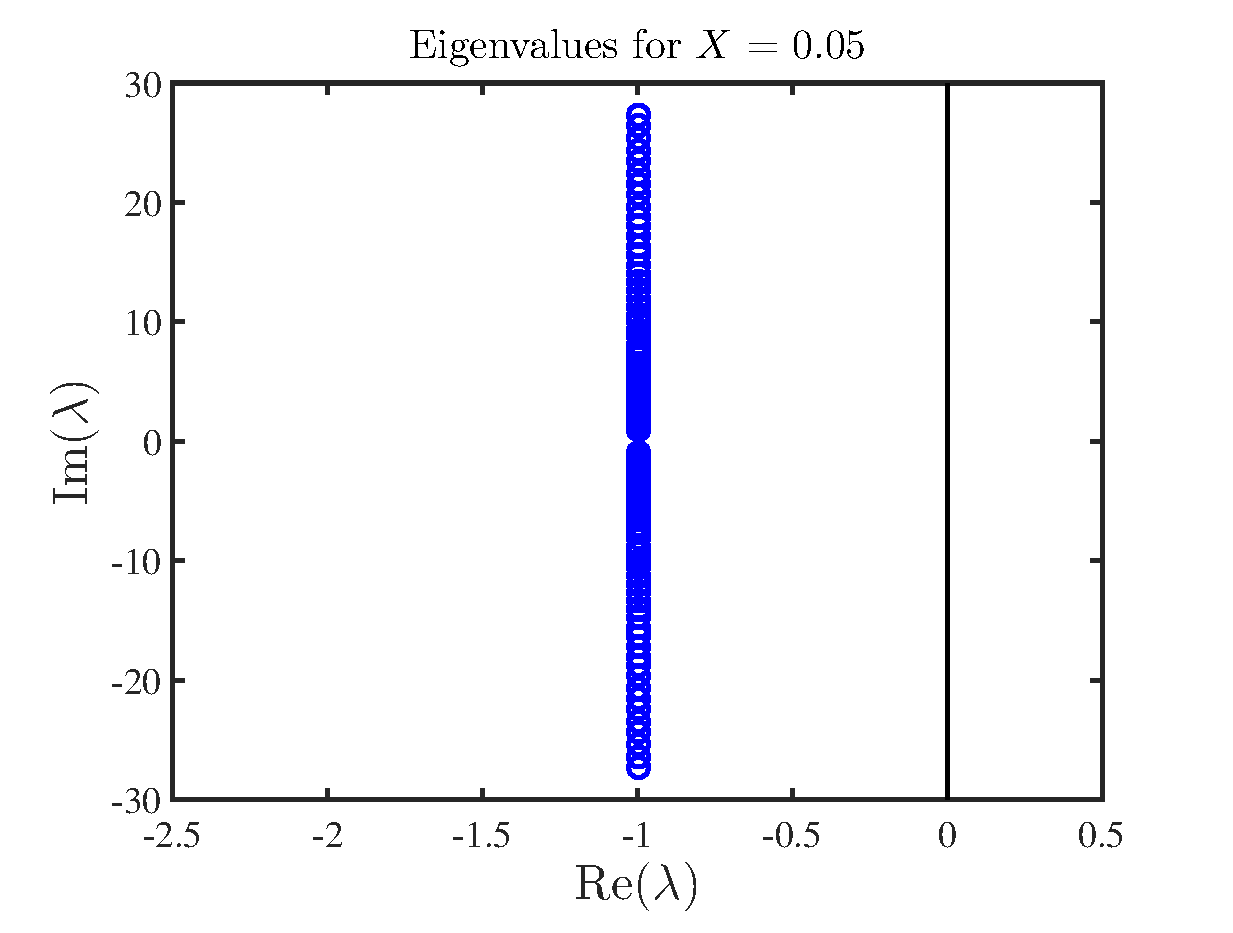
\includegraphics[width=0.5\textwidth]{EigMovieDefense.eps}}{VPlayer.swf}%{StrobeMediaPlayback.swf}
\end{column}
\begin{column}{0.5\textwidth}
\begin{figure}[h]
\centering
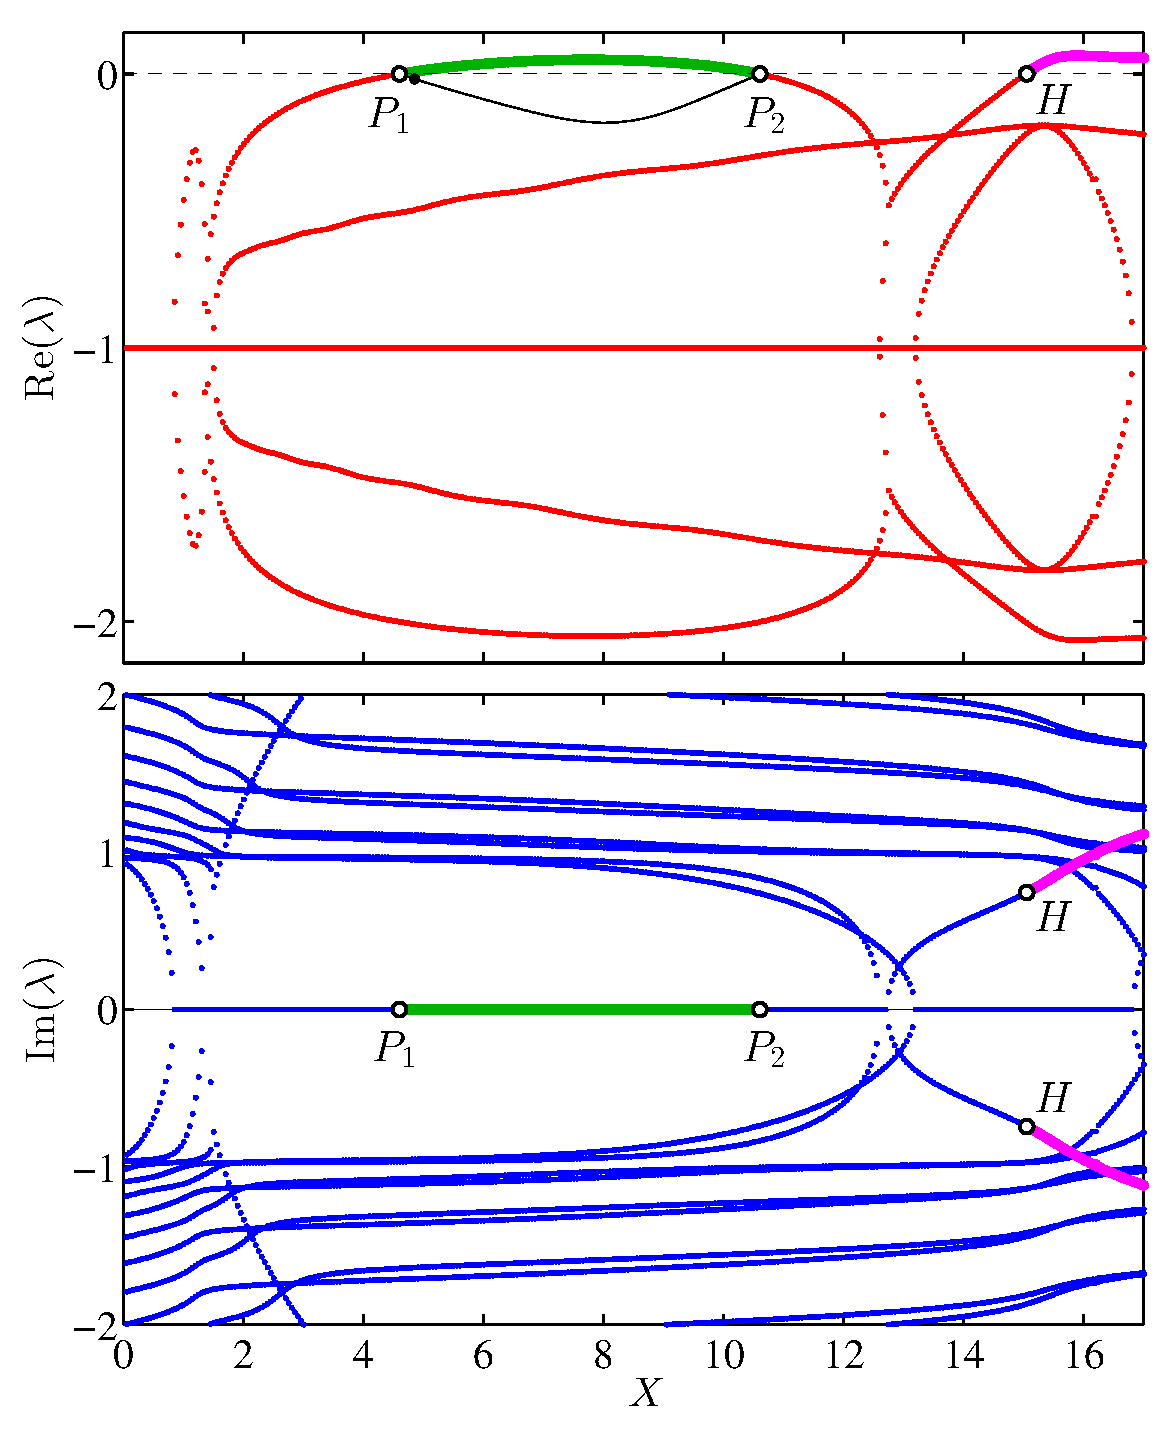
\includegraphics[width=0.9\textwidth]{frequencySpectrumNN.eps}
\caption{Real and Imaginary Eigenvalues for Steady State Solutions of Lugiato-Lefever Equation.}
\end{figure}
\end{column}
\end{columns}
\end{frame}

%Slide 22
\begin{frame}[c]{Applications: SSB}{Soliton Density Evolution}
\begin{columns}
\begin{column}{0.5\textwidth}
\begin{figure}[h]
\centering
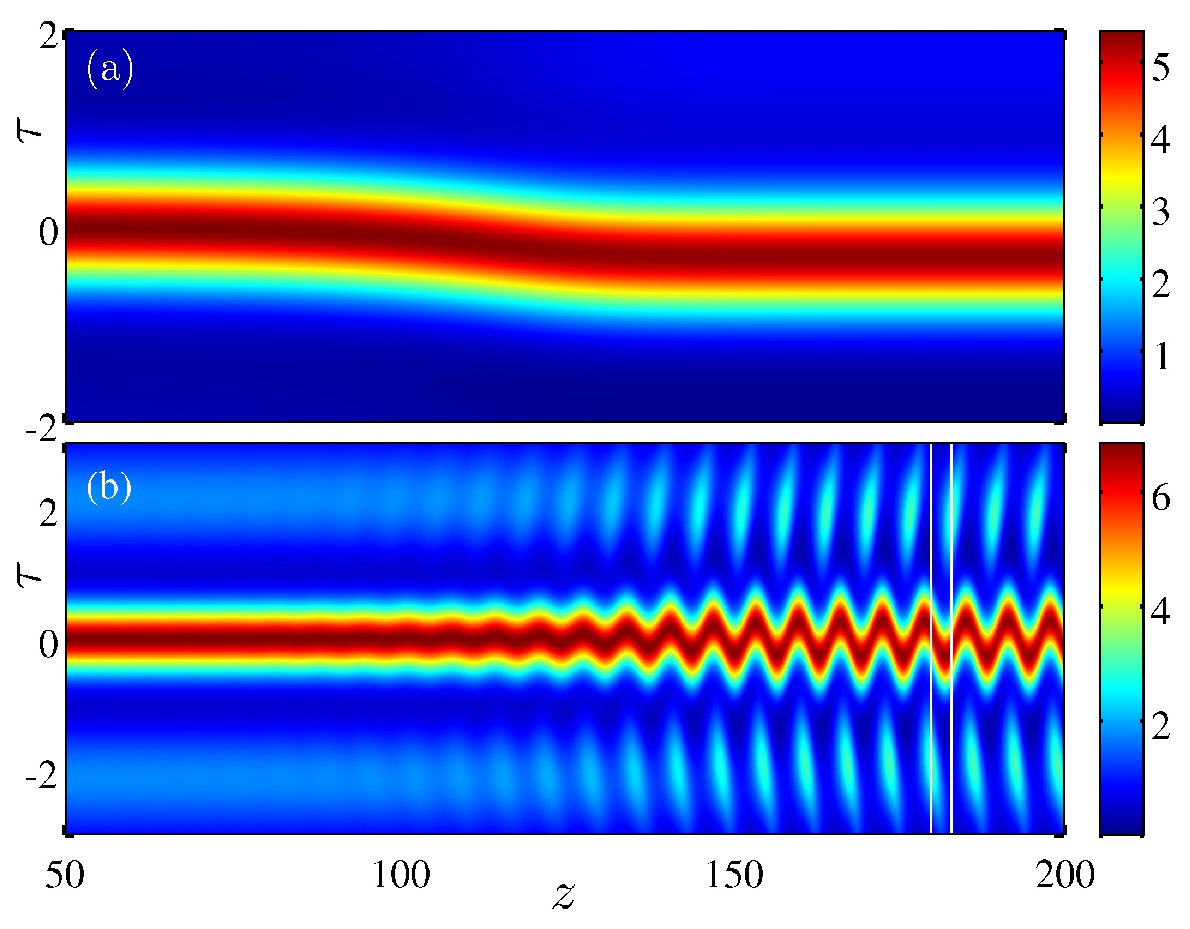
\includegraphics[width=0.85\textwidth]{densityX8X16_t.eps}
%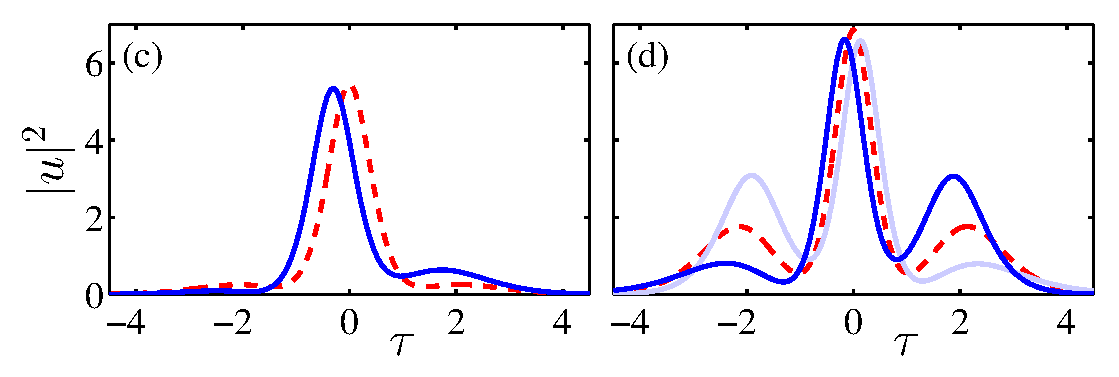
\includegraphics[width=0.85\textwidth]{snaps_X8_X16.eps}
\caption{Evolution of Unstable Symmetric States for (a) $X=8$ between Pitchfork Bifurcations and (b) $X =16$ Periodic Breathing Solution near Hopf Bifurcation.}
\end{figure}
\end{column}
\begin{column}{0.5\textwidth}
\centering
         \includemedia[%
         	%label=pitch,%
 		width=0.8\linewidth,%
  		%height=0.4\linewidth,%
		transparent=true,%
  		activate=onclick,%
		%deactivate=pageclose,%
		%stepping=true,%
  		addresource=densityX8defense.mp4,%
  		flashvars={source=densityX8defense.mp4 &loop=true &controlBarAutoHide=true}%
		]{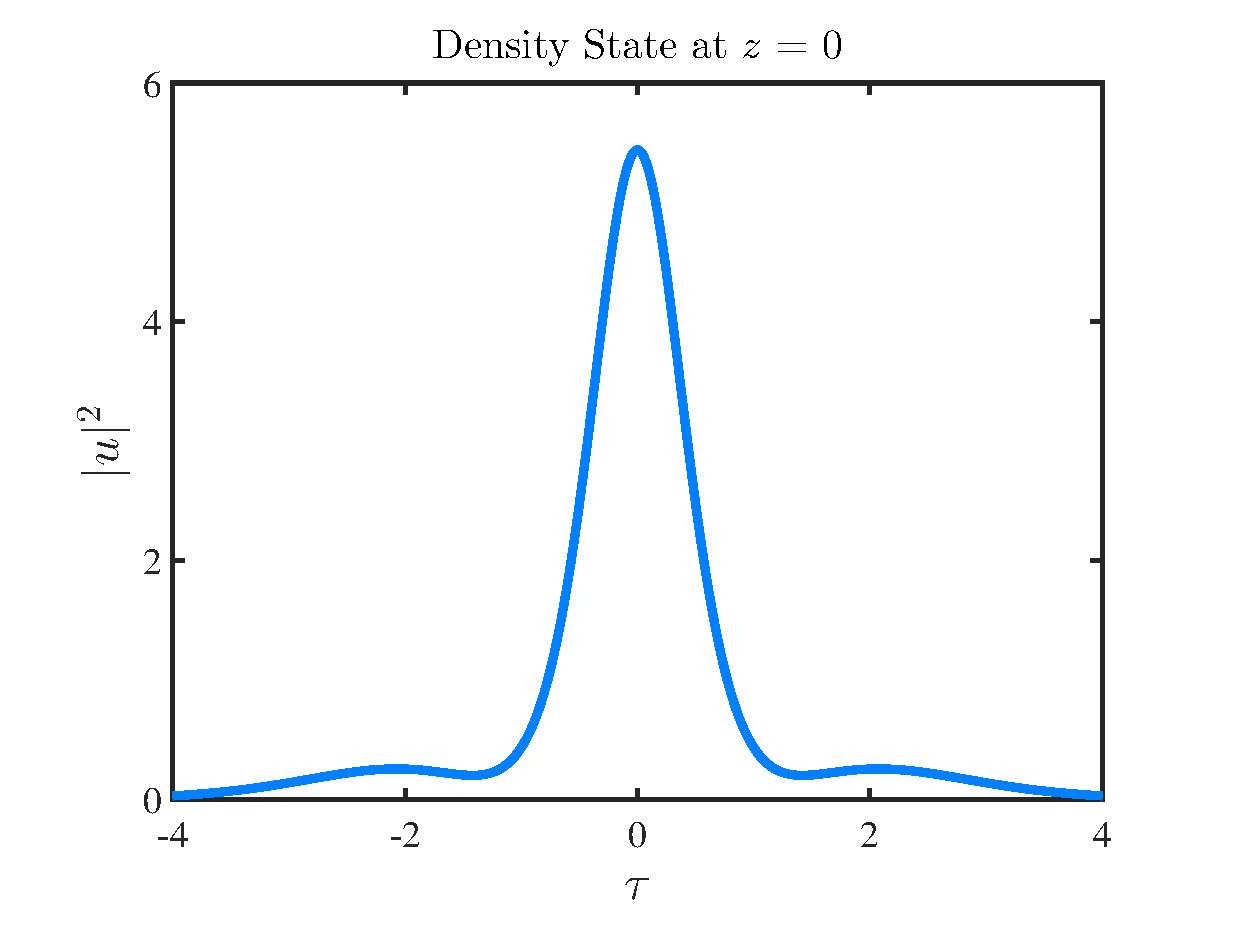
\includegraphics[width=0.5\textwidth]{densityX8defense.eps}}{VPlayer.swf}%{StrobeMediaPlayback.swf}
		\\
		
         \includemedia[%
         	%label=Hopf,%
 		width=0.8\linewidth,%
  		%height=0.4\linewidth,%
		transparent=true,%
  		activate=onclick,%
		%deactivate=pageopen,%
		%stepping=true,%
  		addresource=densityX16defense.mp4,%
  		flashvars={source=densityX16defense.mp4 &loop=true &controlBarAutoHide=true}%
		]{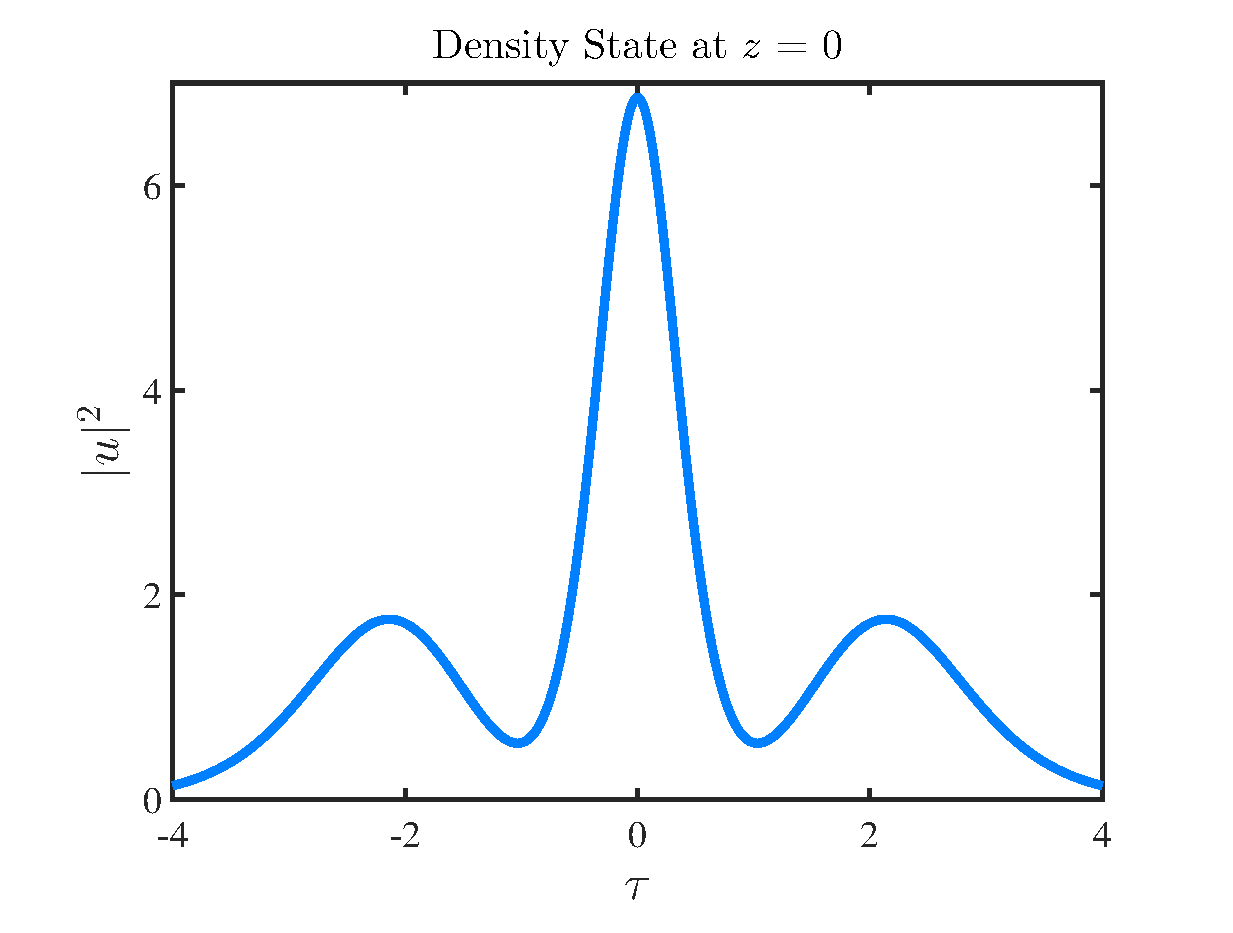
\includegraphics[width=0.5\textwidth]{densityX16defense.eps}}{VPlayer.swf}%{StrobeMediaPlayback.swf}
\end{column}
\end{columns}
\end{frame}

%Slide 23
\begin{frame}[c]{Applications: SSB}{NCVA with $\mathcal{R} = (-i u_+ + i S(\tau))u_-$}
%\vspace{1em}
\textcolor{paleblue}{Ansatz 1}  Four-Parameters
%\vspace{-1em}
\fontsize{9}{9}\textcolor{regal}{\begin{align*} u = a \exp[-(\tau-\xi)^2/2\sigma^2] \exp[ib]   \end{align*}}
%\vspace{-1em}
\textcolor{paleblue}{Ansatz 2} Six-Parameters 
\fontsize{9}{9}\textcolor{regal}{{\begin{align*} 
u = a \exp[-(\tau-\xi)^2/2\sigma^2] \exp[i(d(\tau-\xi)^2 + c(\tau - \xi) + b)] 
\end{align*}}}
\end{frame}

%slide 24
\begin{frame}[c]{Applications: SSB}{NCVA for \textcolor{paleblue}{Ansatz 1} }
\begin{alertblock}{\fontsize{8}{8}{Analytical Expressions - $J = \exp\Bigg[-\frac{\xi^2}{T_0^2+2\sigma^2}\Bigg] \sqrt{P}\sqrt{2} T_0 \sqrt{\pi}$}}
\fontsize{8}{8}{\begin{align*}
\frac{1}{2}\frac{a^2\sqrt{\pi}}{\sigma^2} + \frac{1}{4}a^4\sqrt{2}\sqrt{\pi} = \frac{8 J \xi^2 \sigma^2 a  \sin(b)}{(T_0^2+2\sigma^2)^{5/2}}+ \frac{2 J a \sin(b)T _0^2 }{(T_0^2+2\sigma^2)^{3/2}}+ \Delta a^2 \sqrt{\pi}, \\
0 = -2 a^2 \sigma \sqrt{\pi}+\frac{2 J a\cos(b) \sigma }{\sqrt{T_0^2+2\sigma^2}}, \\
- \frac{a \sqrt{\pi}}{\sigma}+a^3 \sqrt{2}\sigma \sqrt{\pi} = \frac{2 J \sin(b) \sigma}{\sqrt{T_0^2+2\sigma^2}}+2\Delta a\sigma \sqrt{\pi}, \\
0 = -\frac{4 J a \xi \sigma \sin(b)}{(T_0^2+2\sigma^2)^{3/2}}.
\end{align*}}
\end{alertblock}
\end{frame}


%SLide 25
\begin{frame}[c]{Applications: SSB}{NCVA for SSB \textcolor{paleblue}{Ansatz 1}}
\vspace{-1em}
\begin{figure}[h]
\centering
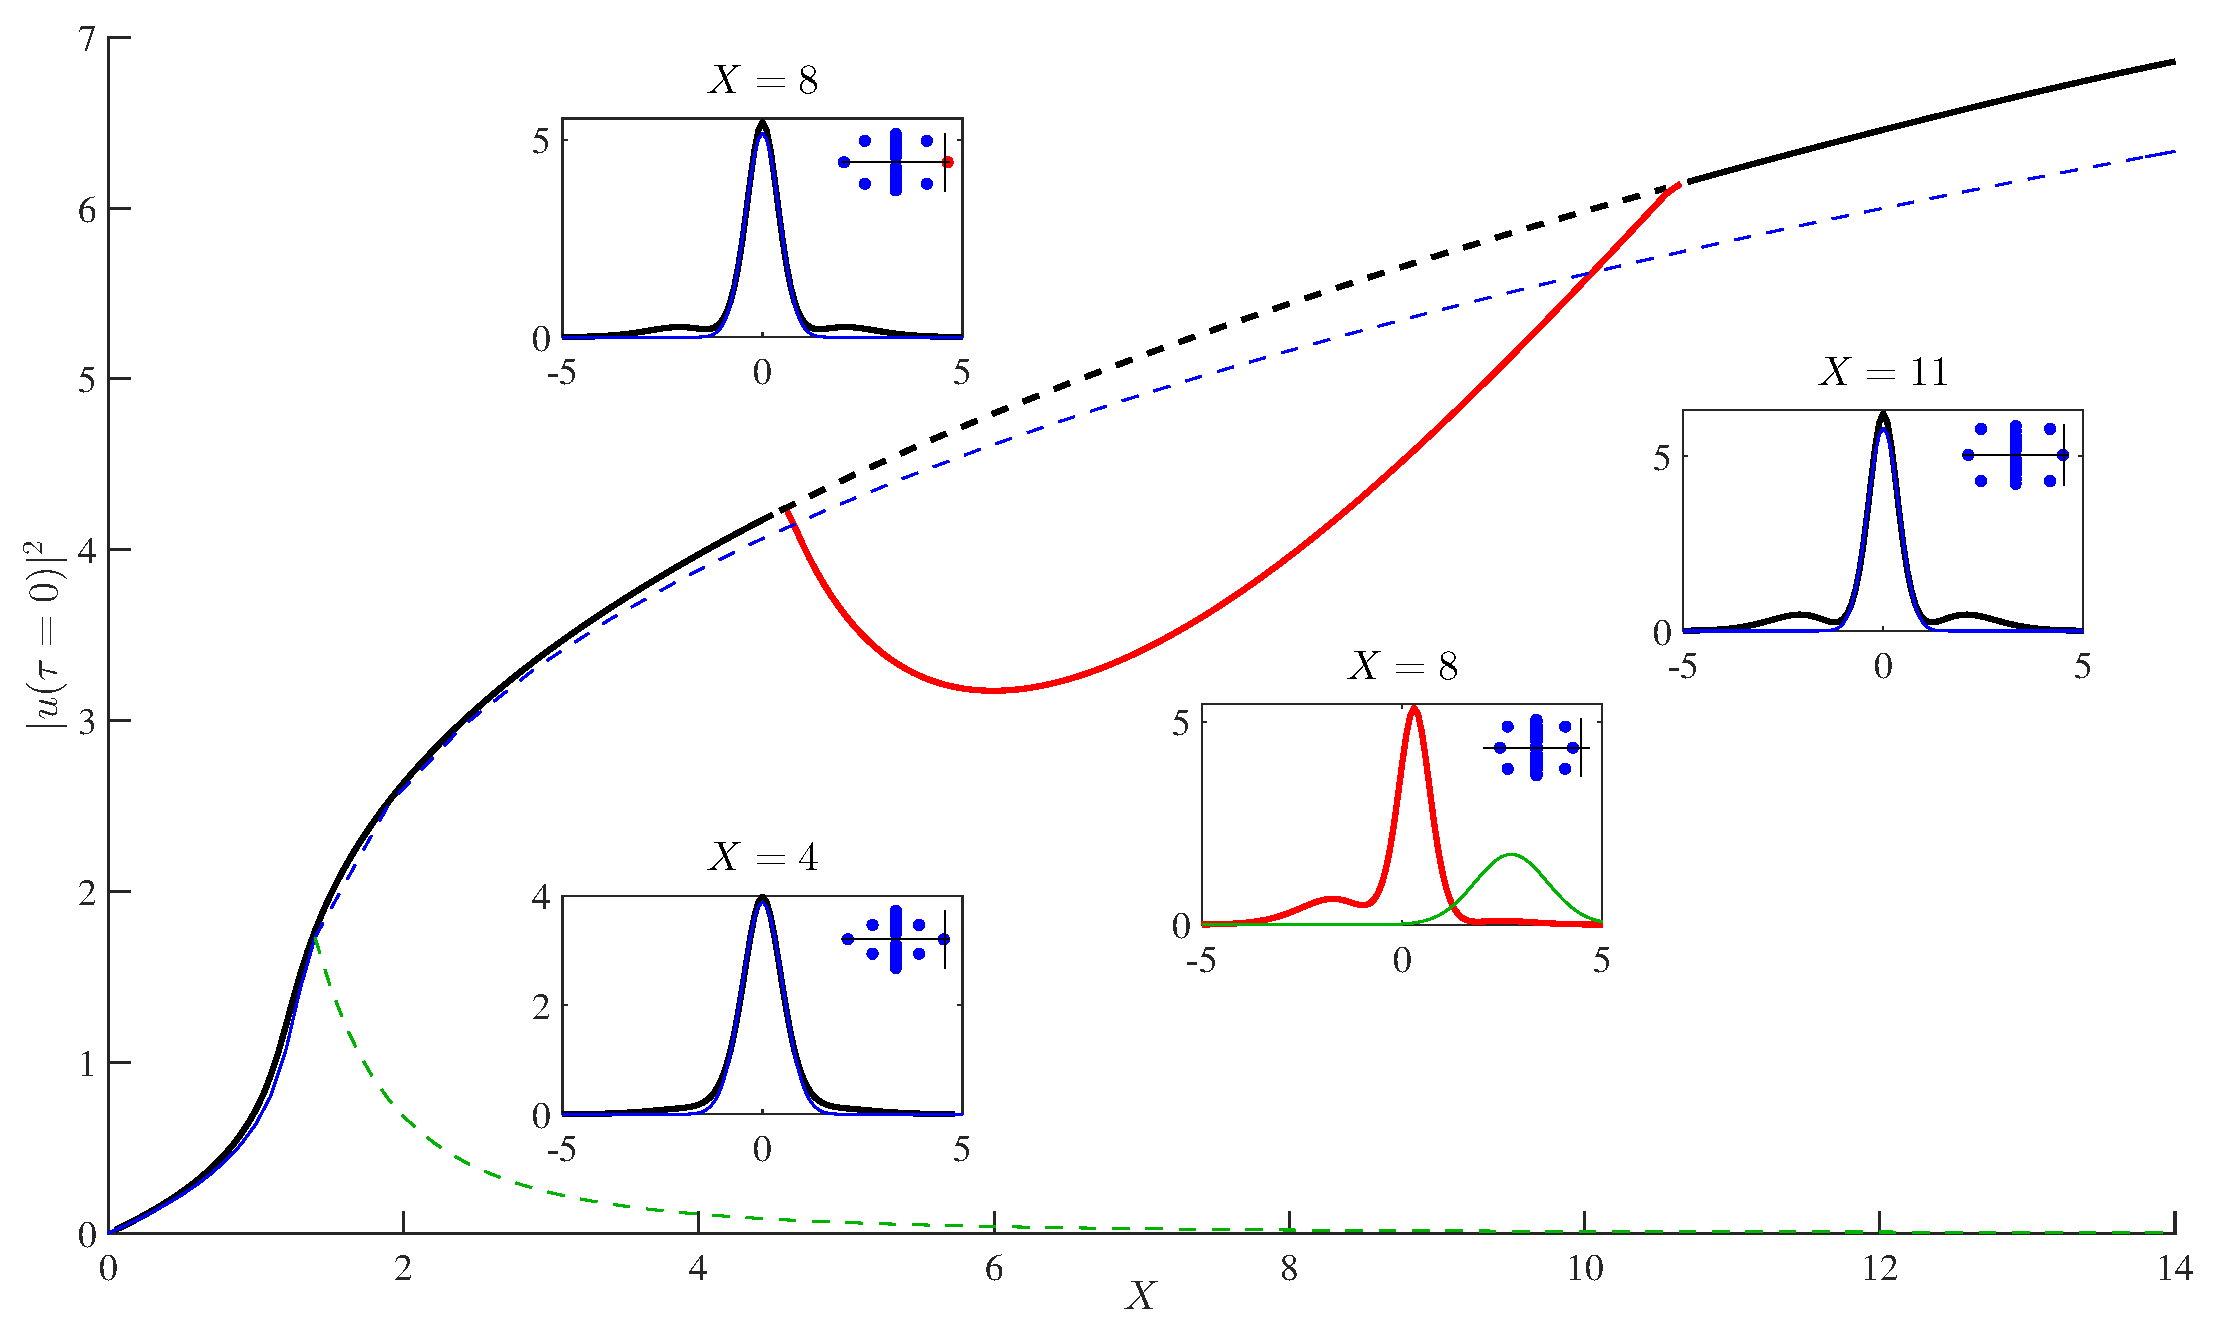
\includegraphics[width =0.9\textwidth]{SSBBif4PN.ps}
\caption{Bifurcation for steady states of the LL model and their approximation using the NCVA.}
\end{figure}
\end{frame}

%Slide 26
\begin{frame}[c]{Applications: SSB}{Fluid Velocity $\nabla \phi$ of LL Equation \& NCVA Solutions}
\begin{figure}[h]
\centering
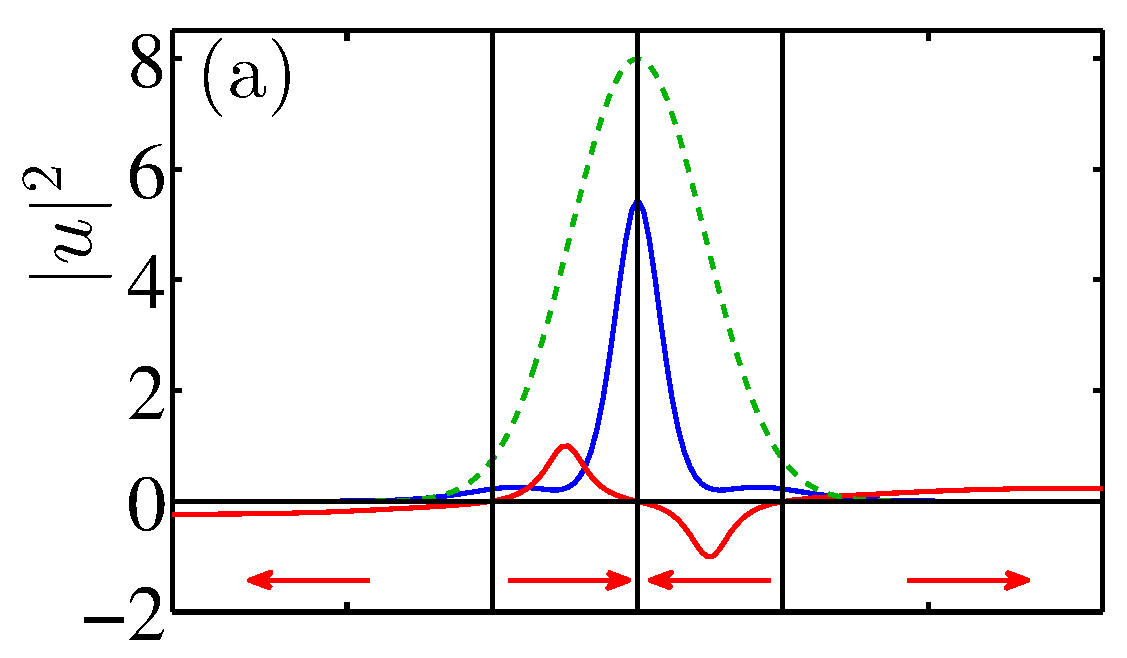
\includegraphics[width=0.32\textwidth]{fluidVelocity_X8_pdeSN.eps} \quad
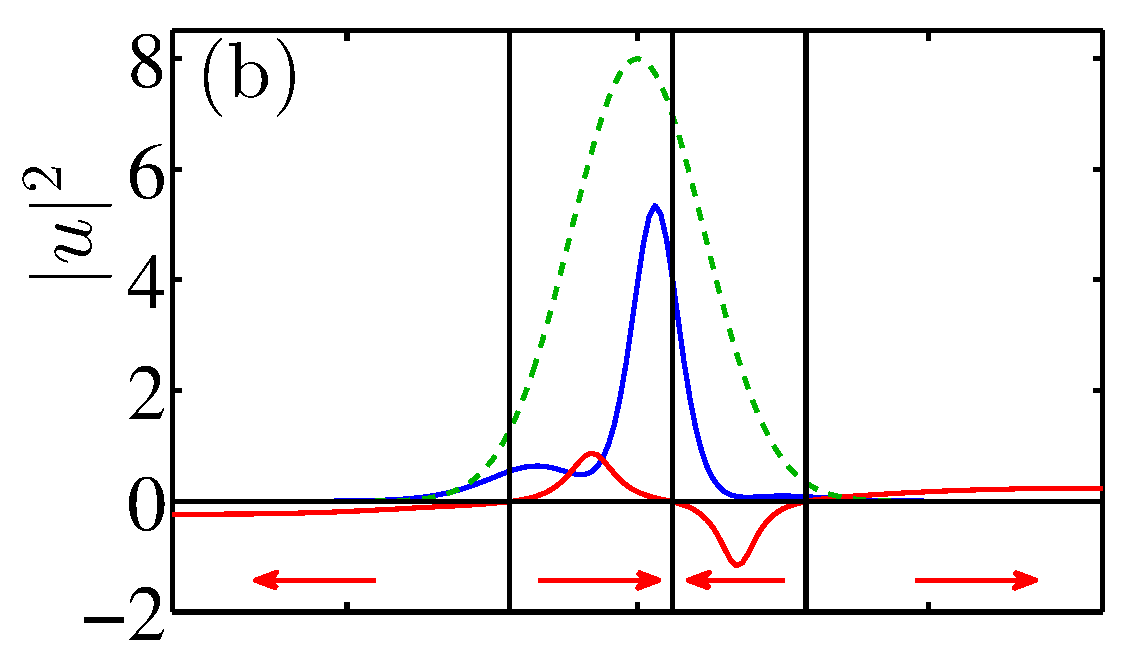
\includegraphics[width=0.32\textwidth]{fluidVelocity_X8_pdeASN.eps} 
\\
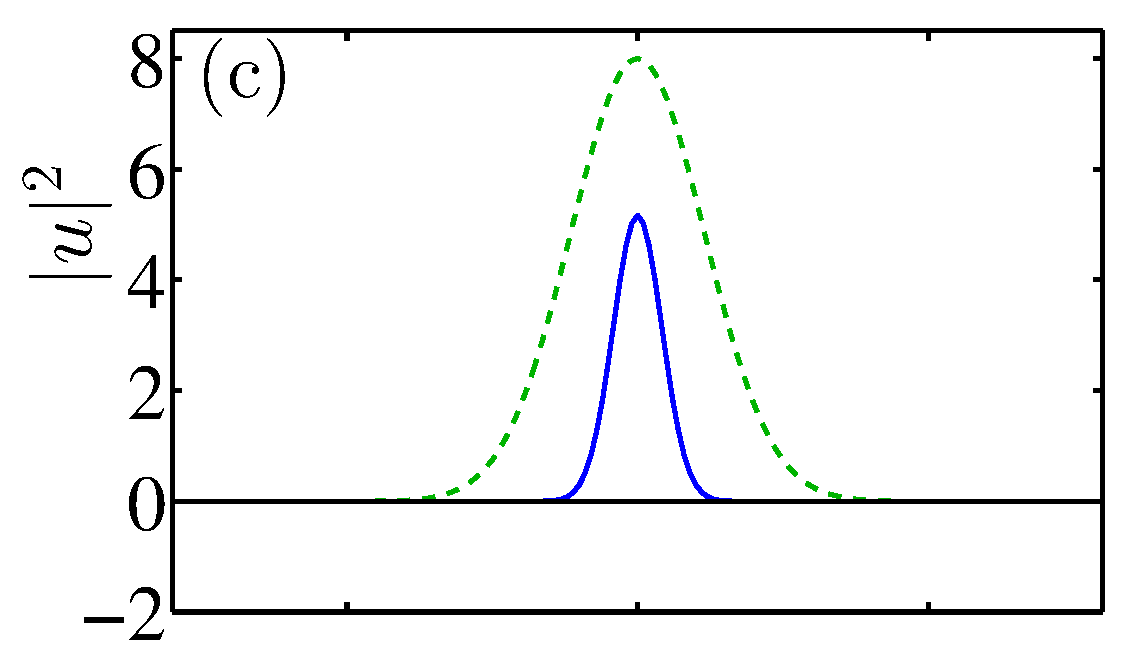
\includegraphics[width=0.32\textwidth]{fluidVelocity_X8_4PSN.eps} \quad
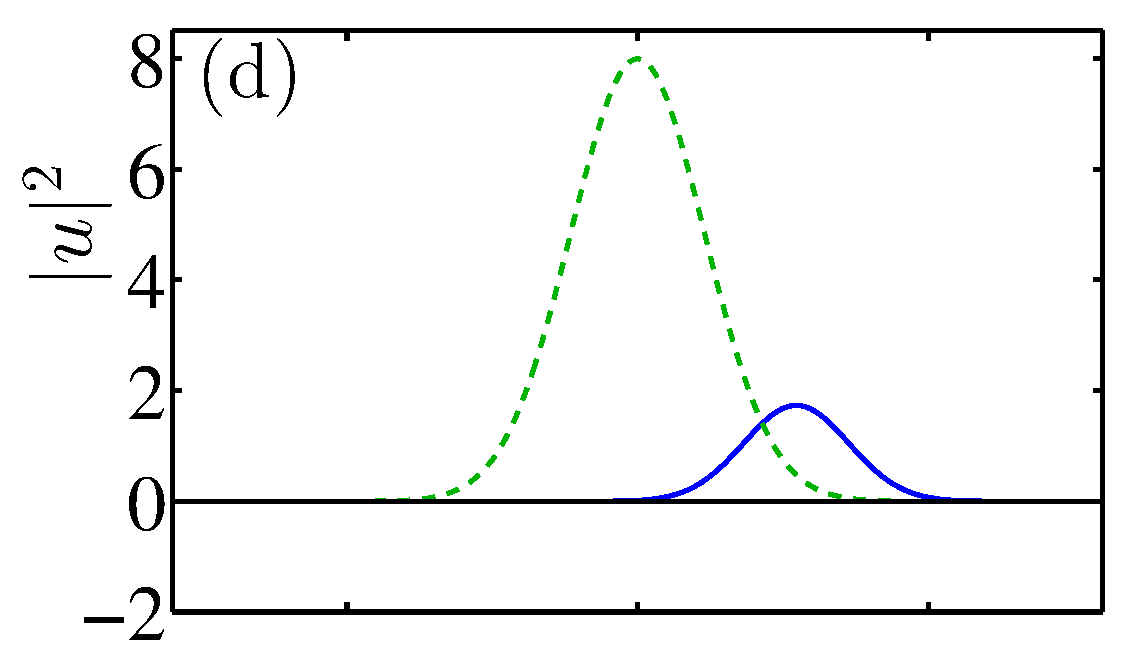
\includegraphics[width=0.32\textwidth]{fluidVelocity_X8_4PASN.eps} 
\\
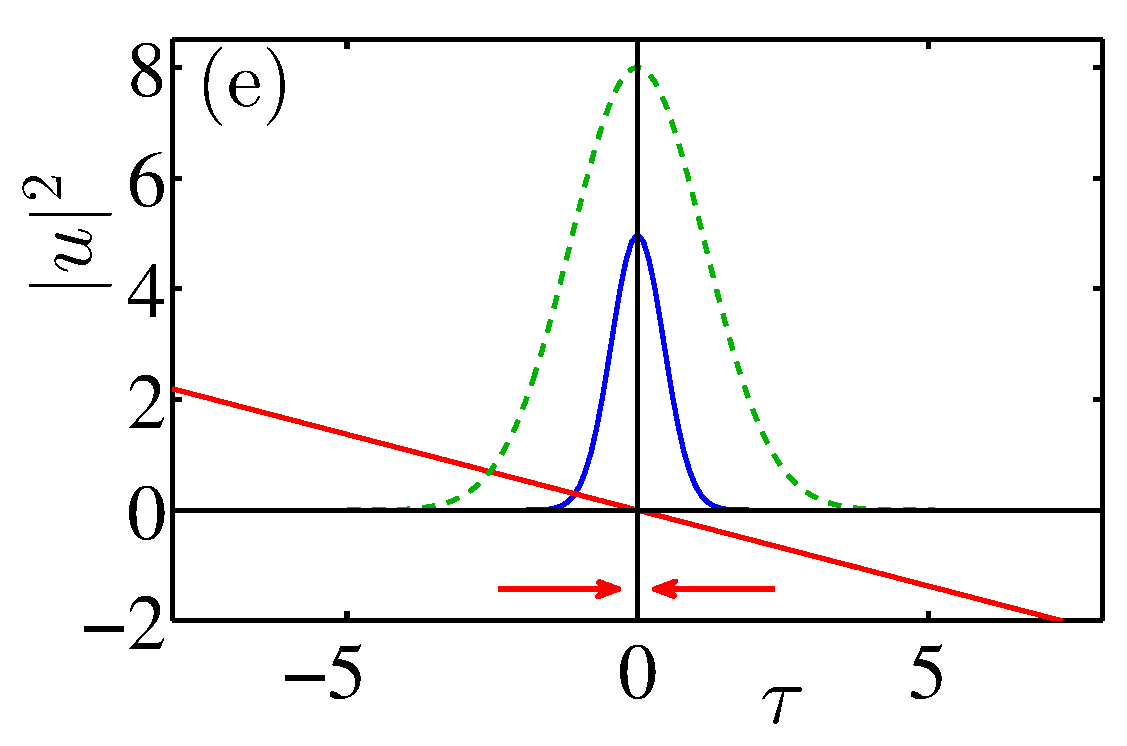
\includegraphics[width=0.32\textwidth]{fluidVelocity_X8_6PSN.eps} \quad
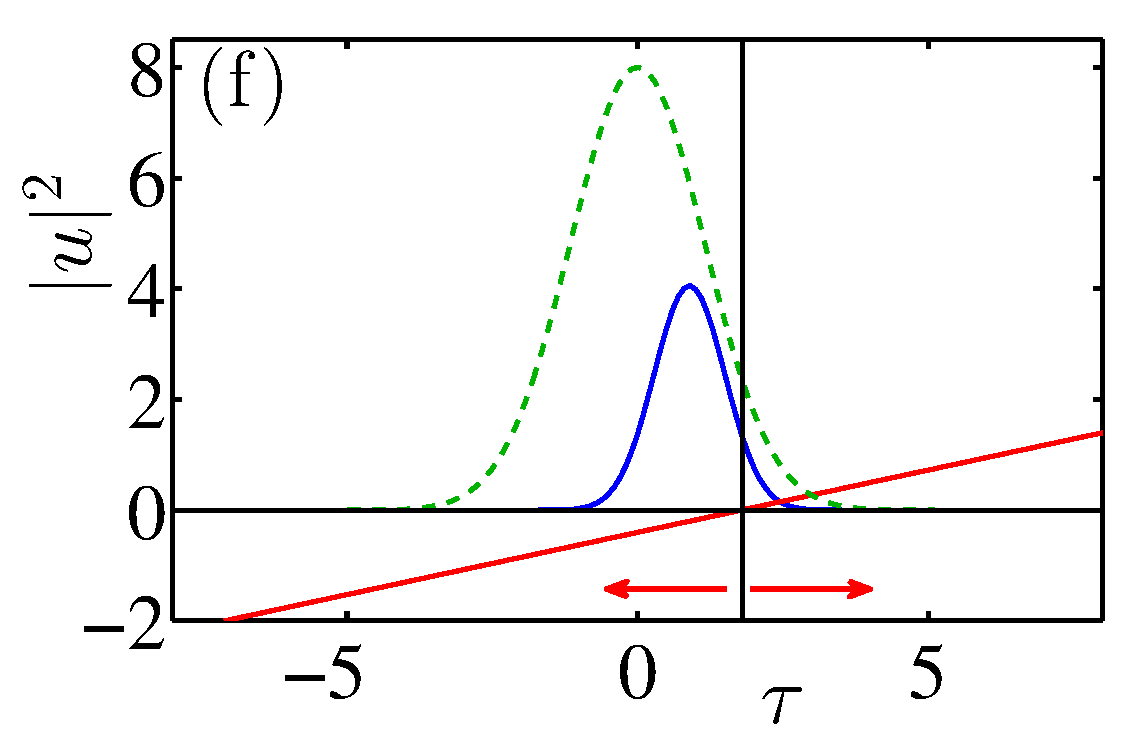
\includegraphics[width=0.32\textwidth]{fluidVelocity_X8_6PASN.eps}
\caption{The (red) arrows indicate the direction of the fluid velocity which drives 
the SSB bifurcation between the symmetric and asymmetric solutions.}
\end{figure}
\end{frame}

%Slide 26
\begin{frame}[c]{Applications: SSB}{NCVA for \textcolor{paleblue}{Ansatz 2} }%with $\mathcal{R} = (-i u_+ + i S(\tau))u_-$}
%\vspace{-1em}
%\textcolor{paleblue}{Ansatz 2}
%\vspace{-0.5em}
%\fontsize{9}{9}\textcolor{regal}{{\begin{align*} 
%u = a \exp[-(\tau-\xi)^2/2\sigma^2] \exp[i(d(\tau-\xi)^2 + c(\tau - \xi) + b)] 
%\end{align*}}}
%\vspace{-1.5em}
%\begin{columns}
%\begin{column}{0.7\textwidth}
\begin{alertblock}{ODEs}
%\vspace{-2em}
\fontsize{7}{7}{ \begin{align*}
\dot{a} &= \frac{1}{4}\frac{-4a^2\sigma^3\sqrt{\pi}+3\sigma^2I_b-8a^2d\sigma^3\sqrt{\pi}-2I_d}{a\sigma^3\sqrt{\pi}}, \\
\dot{b} &= -\frac{1}{8}\frac{8a^2\sqrt{\pi}-5a^4\sqrt{2}\sqrt{\pi}\sigma^2-4I_\sigma \sigma^2+6I_a\sigma a-8a^2c^2\sqrt{\pi}\sigma^2-8\sigma c I_c+8a^2 \Delta\sqrt{\pi}\sigma^2}{a^2\sigma^2\sqrt{\pi}}, \\
\dot{c} &= -\frac{c I_b+I_{\xi}}{a^2\sigma\sqrt{\pi}}, \\
\dot{d}&= \frac{1}{4}\frac{4a^2\sqrt{\pi}-16a^2 d^2 \sigma^4\sqrt{\pi}-a^4\sqrt{2}\sqrt{\pi}\sigma^2-4I_s\sigma^2+2I_a\sigma a}{a^2\sigma^4\sqrt{\pi}}, \\
\dot{\sigma}&= -\frac{1}{2}\frac{\sigma^2I_b-8a^2 d \sigma^3\sqrt{\pi}-2I_d}{a^2\sigma^2\sqrt{\pi}}, \\
\dot{\xi} &= \frac{2a^2\sigma c \sqrt{\pi}+I_c}{a^2\sigma\sqrt{\pi}}. 
\end{align*}}
\end{alertblock}
%\end{column}
%\begin{column}{0.3\textwidth}
\end{frame}

\begin{frame}[c]{Applications: SSB}{NCVA for \textcolor{paleblue}{Ansatz 2} }%with $\mathcal{R} = (-i u_+ + i S(\tau))u_-$}
\begin{block}{Integrals}
\fontsize{9}{9}{With  $\Phi =d(\tau-\xi)^2+c(\tau-\xi)+b$  and  $E = 2\sqrt{X} e^{-\frac{ (\tau-\xi)^2}{2 \sigma^2}}e^{-\frac{\tau^2}{T_0^2}} $:}
\fontsize{7}{7}{\begin{align*}
\begin{matrix}  I_a = \int  E \sin(\Phi) \,d\tau, & 
I_b = \int  a E \cos(\Phi) \,d\tau, \\[0em]
I_c = \int  a E (\tau-\xi) \cos(\Phi) \,d\tau,  & 
I_d  = \int a E (\tau-\xi)^2 \cos(\Phi) \,d\tau ,\\[0em] 
I_\sigma =\int \frac{a E}{\sigma^3} \sin(\Phi) \,d\tau,   &
I_\xi =\int  \Big[ aE \left(-2d(\tau-\xi)-c\right) \cos(\Phi)  + \frac{a E (\tau-\xi) }{\sigma^2} \sin(\Phi) \Big] \,d\tau.
\end{matrix}
\end{align*}}
%
\end{block}
%\end{column}
%\end{columns}
\end{frame}


%Slide 27
\begin{frame}[c]{Applications: SSB}{NCVA for SSB \textcolor{paleblue}{Ansatz 2}}
\vspace{-1em}
\begin{figure}[H!]
\centering
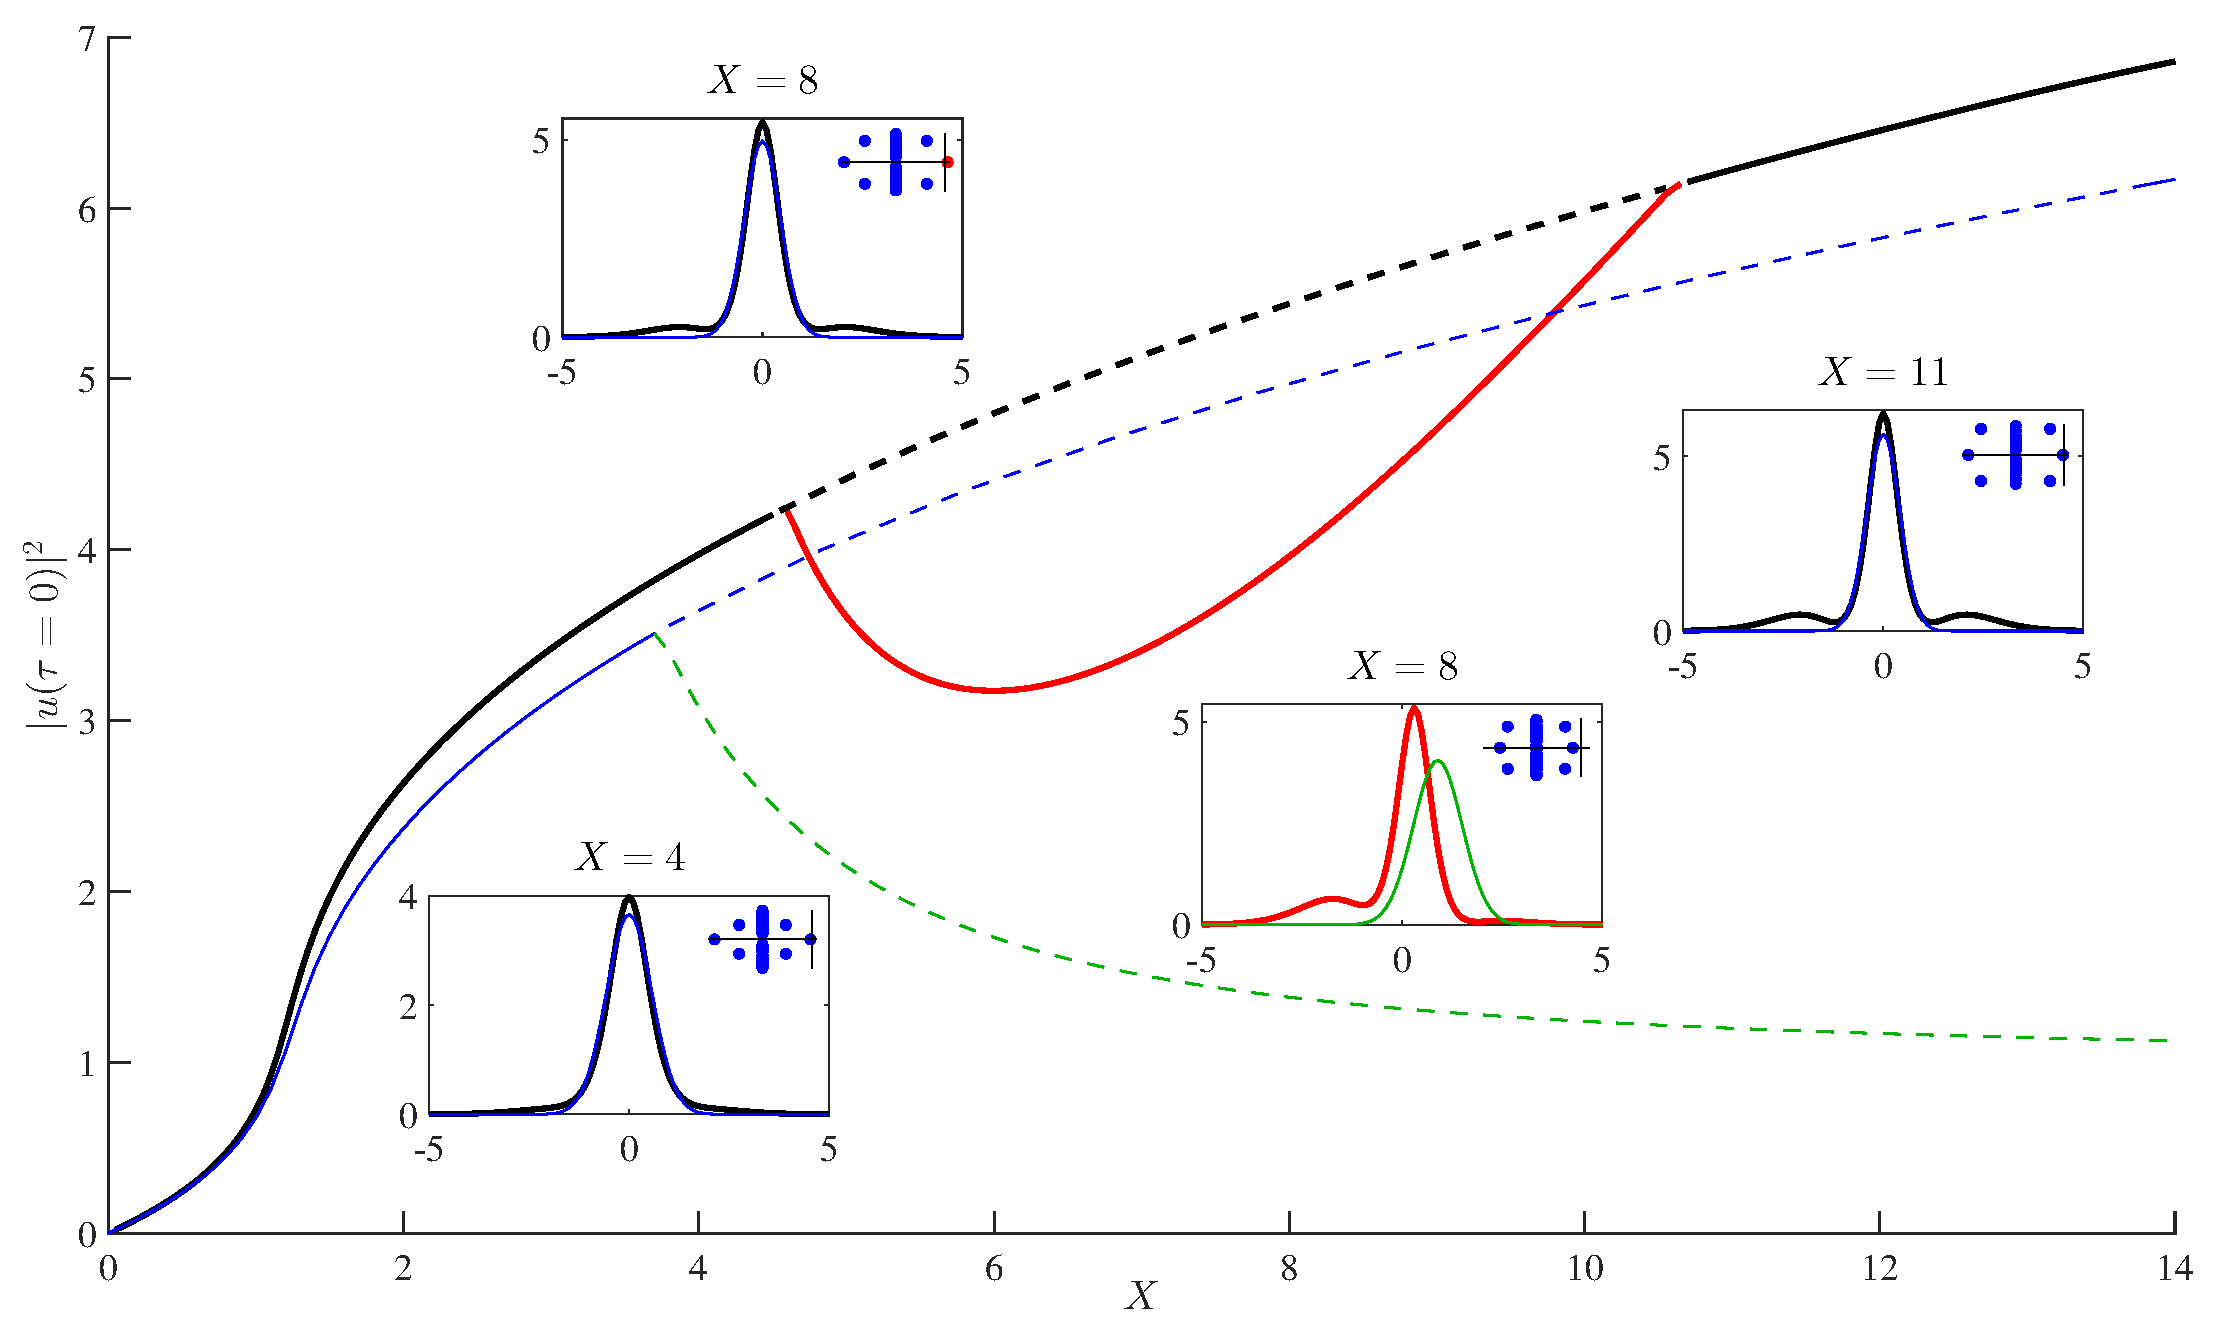
\includegraphics[width = 0.9\textwidth]{SSBBif6PN.ps}
\caption{Bifurcation for steady states of the LL model and their approximation using the NCVA.}
\end{figure}
\end{frame}

%Slide 28
\begin{frame}[c]{Applications: SSB}{NCVA ODE Linearization Spectrum}
\begin{columns}
\begin{column}{0.5\textwidth}
\begin{figure}[h]
\centering
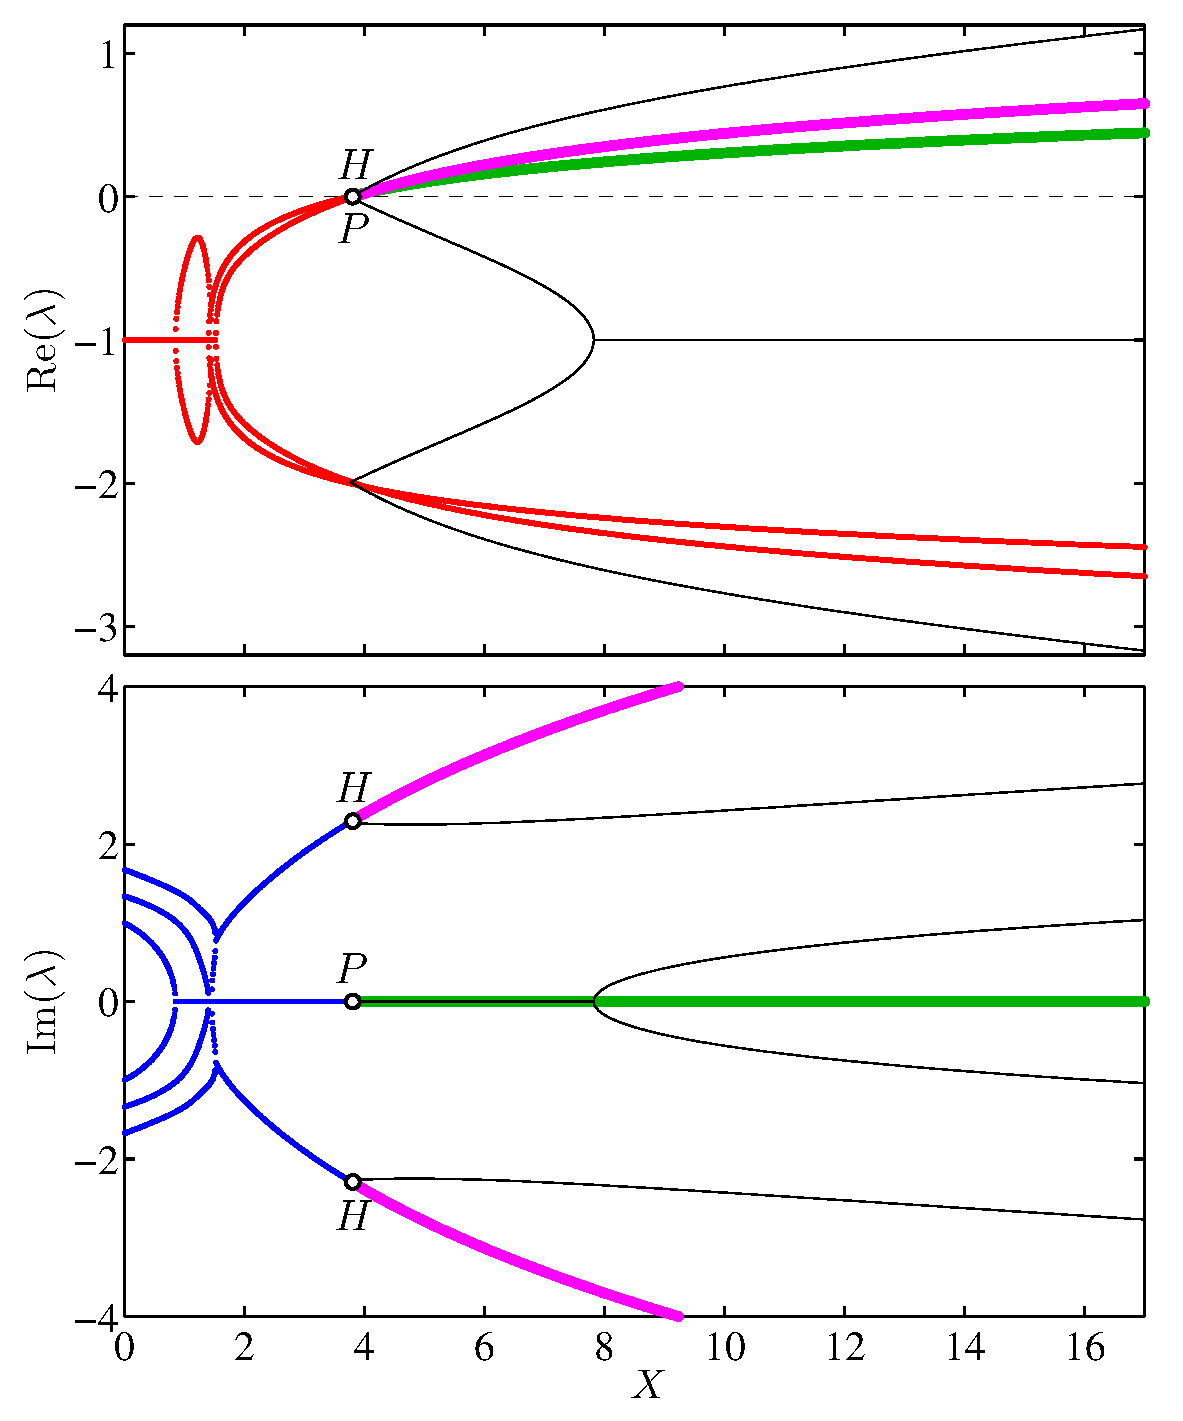
\includegraphics[height=0.6\textheight]{frequencySpectrum_NCVA.eps}
\caption{
Linearization spectrum for the reduced NCVA ODE.   Degenerate bifurcation with simultaneous pitchfork (P) and Hopf (H)
bifurcations. % (\ref{6pE}).
%The notation is the same as the spectrum for the original LL model
%depicted in Fig.~\ref{fig:frequencySpectrum}.
%%
%The reduced ODE model displays a degenerate bifurcation
%consisting of simultaneous pitchfork (P) and Hopf (H)
%bifurcations and thus the asymmetric steady state (see thin black
%solid lines) is unstable from its inception.
}
\end{figure}
\end{column}
\begin{column}{0.5\textwidth}
\centering
\vspace{5em}
         \includemedia[%
 		width=0.9\linewidth,%
		transparent=true,%
  		activate=onclick,%
  		addresource=EigNCVAMovieDefense.mp4,%
  		flashvars={source=EigNCVAMovieDefense.mp4 &loop=true &controlBarAutoHide=true}%
		]{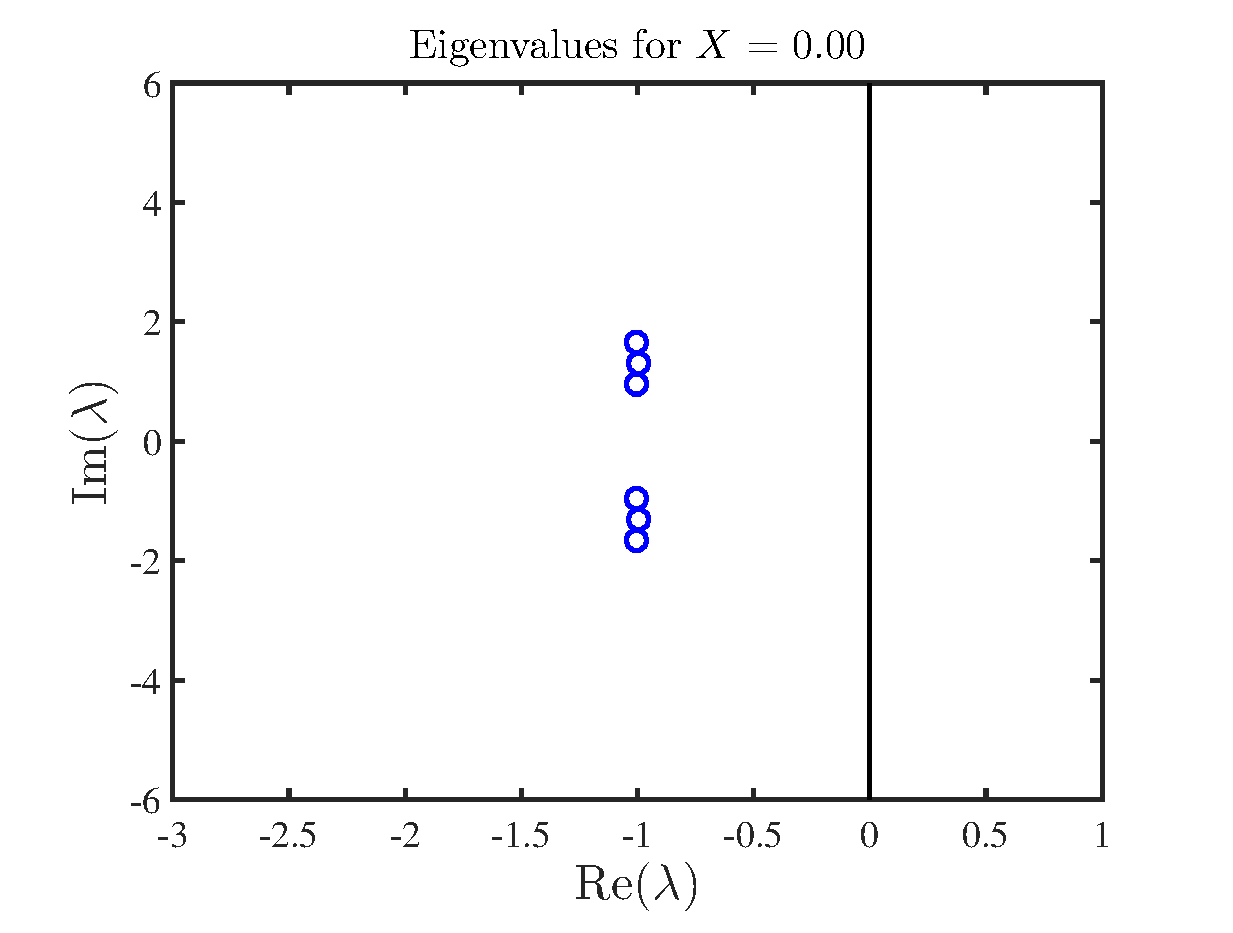
\includegraphics[width=0.5\textwidth]{EigNCVAMovieDefense.eps}}{VPlayer.swf}%{StrobeMediaPlayback.swf}
\end{column}
\end{columns}
\end{frame}

%SLide 29
\begin{frame}[c]{Applications: SSB}{Local Bifurcation Analysis}
Dynamical systems approach based on a center manifold reduction close to \textcolor{turtlegreen}{pitchfork bifurcations}.
\\
\vspace{1em}
\fontsize{9}{9}{\begin{itemize}
\item Start by defining $U = U_X + \nu$ and $V = V_X + v$ (symmetric steady state solutions ($U_X, V_X$) with deviations $\nu$ and $v$). 
%\begin{eqnarray*}
%U = U_X + \nu, \quad \quad V = V_X + v.
%\end{eqnarray*}
\item Results in new dynamical system 
\textcolor{regal}{\begin{align*}
w_z = \mathcal{A}_Xw + \mathcal{J}(\mathcal{R}_{2} (w, w) + \mathcal{R}_3 (w)),
\end{align*}}
in which $w = (\nu, v)^T$ and $\mathcal{A}_X$ is the matrix linear operator  
\begin{align*}
\mathcal{A}_X = -\mathbb{I} + \mathcal{J}\mathcal{L}_X,  
\label{Ax}
\end{align*}
with identity map $\mathbb{I}$, linear operator $\mathcal{L}_X$, bilinear map $\mathcal{R}_{2} (w_1, w_2)$, and cubic map $\mathcal{R}_{3} (w)$.
\end{itemize}}
\end{frame}

%Slide 
\begin{frame}[c]{Applications:SSB}{Local Bifurcation Analysis Continued}
\fontsize{9}{9}{
\begin{itemize}
\item By arguing with center manifold theorem, this system has 1-D center manifold for any $X$ close to $X_*$ with bounded solutions of form:
\begin{align*}
w(z) = A(z)\zeta_* + \Phi (A(z), X), 
\end{align*}
where $\zeta_*$ are eigenvectors in the kernels of $\mathcal{A}_*$ and $\langle \Phi(A, X), \zeta_*^* \rangle = 0.$
\item Dynamics of center manifold determined by scalar ODE:
\textcolor{turtlegreen}{\begin{align*}
\frac{dA}{dz} = f(A, X) = c_0 (X) A + c_3 A^3 + \mathcal{O} (|A|^3 (|X-X_*| + A^2) ),
\end{align*}}
with real constants $c_0(X) = \lambda_0 (X)$ and 
\begin{align*}
c_3 = \frac{1}{\langle \zeta_*, \mathcal{J} \zeta_2 \rangle} \left( \langle 2 \mathcal{R}_{*,2}(\zeta_*, \Phi_2), \zeta_2 \rangle + \langle \mathcal{R}_3(\zeta_*), \zeta_2 \rangle \right),
\nonumber
\end{align*}
where $\mathcal{A}_{*} \Phi_2 = - \mathcal{J} R_{*,2}(\zeta_*, \zeta_*).$
\end{itemize}}
\end{frame}

%SLide 30
%Change Galerkin to center manifold approach
\begin{frame}[c]{Applications: SSB}{LL Model and Center Manifold Comparison near Pitchfork Bifurcation Points}
\vspace{1em}
%\fontsize{9}{9}{ From linearization spectrum: $c_0(X) = \lambda_0 (X)$ and 
%\begin{align*}
% c_3<0, \; \mbox{~for~} \;  X=X_1, \mbox{~and~}  \;
%  c_3>0, \; \mbox{~for~}  \; X=X_2.
%\end{align*}
{\small Compare to LL model through asymmetry coefficient} \fontsize{8}{8}{$\alpha(X)$
\begin{align*}
u_{\mathrm{Asym} }(X_* + \delta X)\approx u_{\mathrm{Sym} }(X_* + \delta X) + 
\alpha(X_* + \delta X)\, \zeta_*.
\end{align*}}
\vspace{-1em}
\begin{figure}
\centering
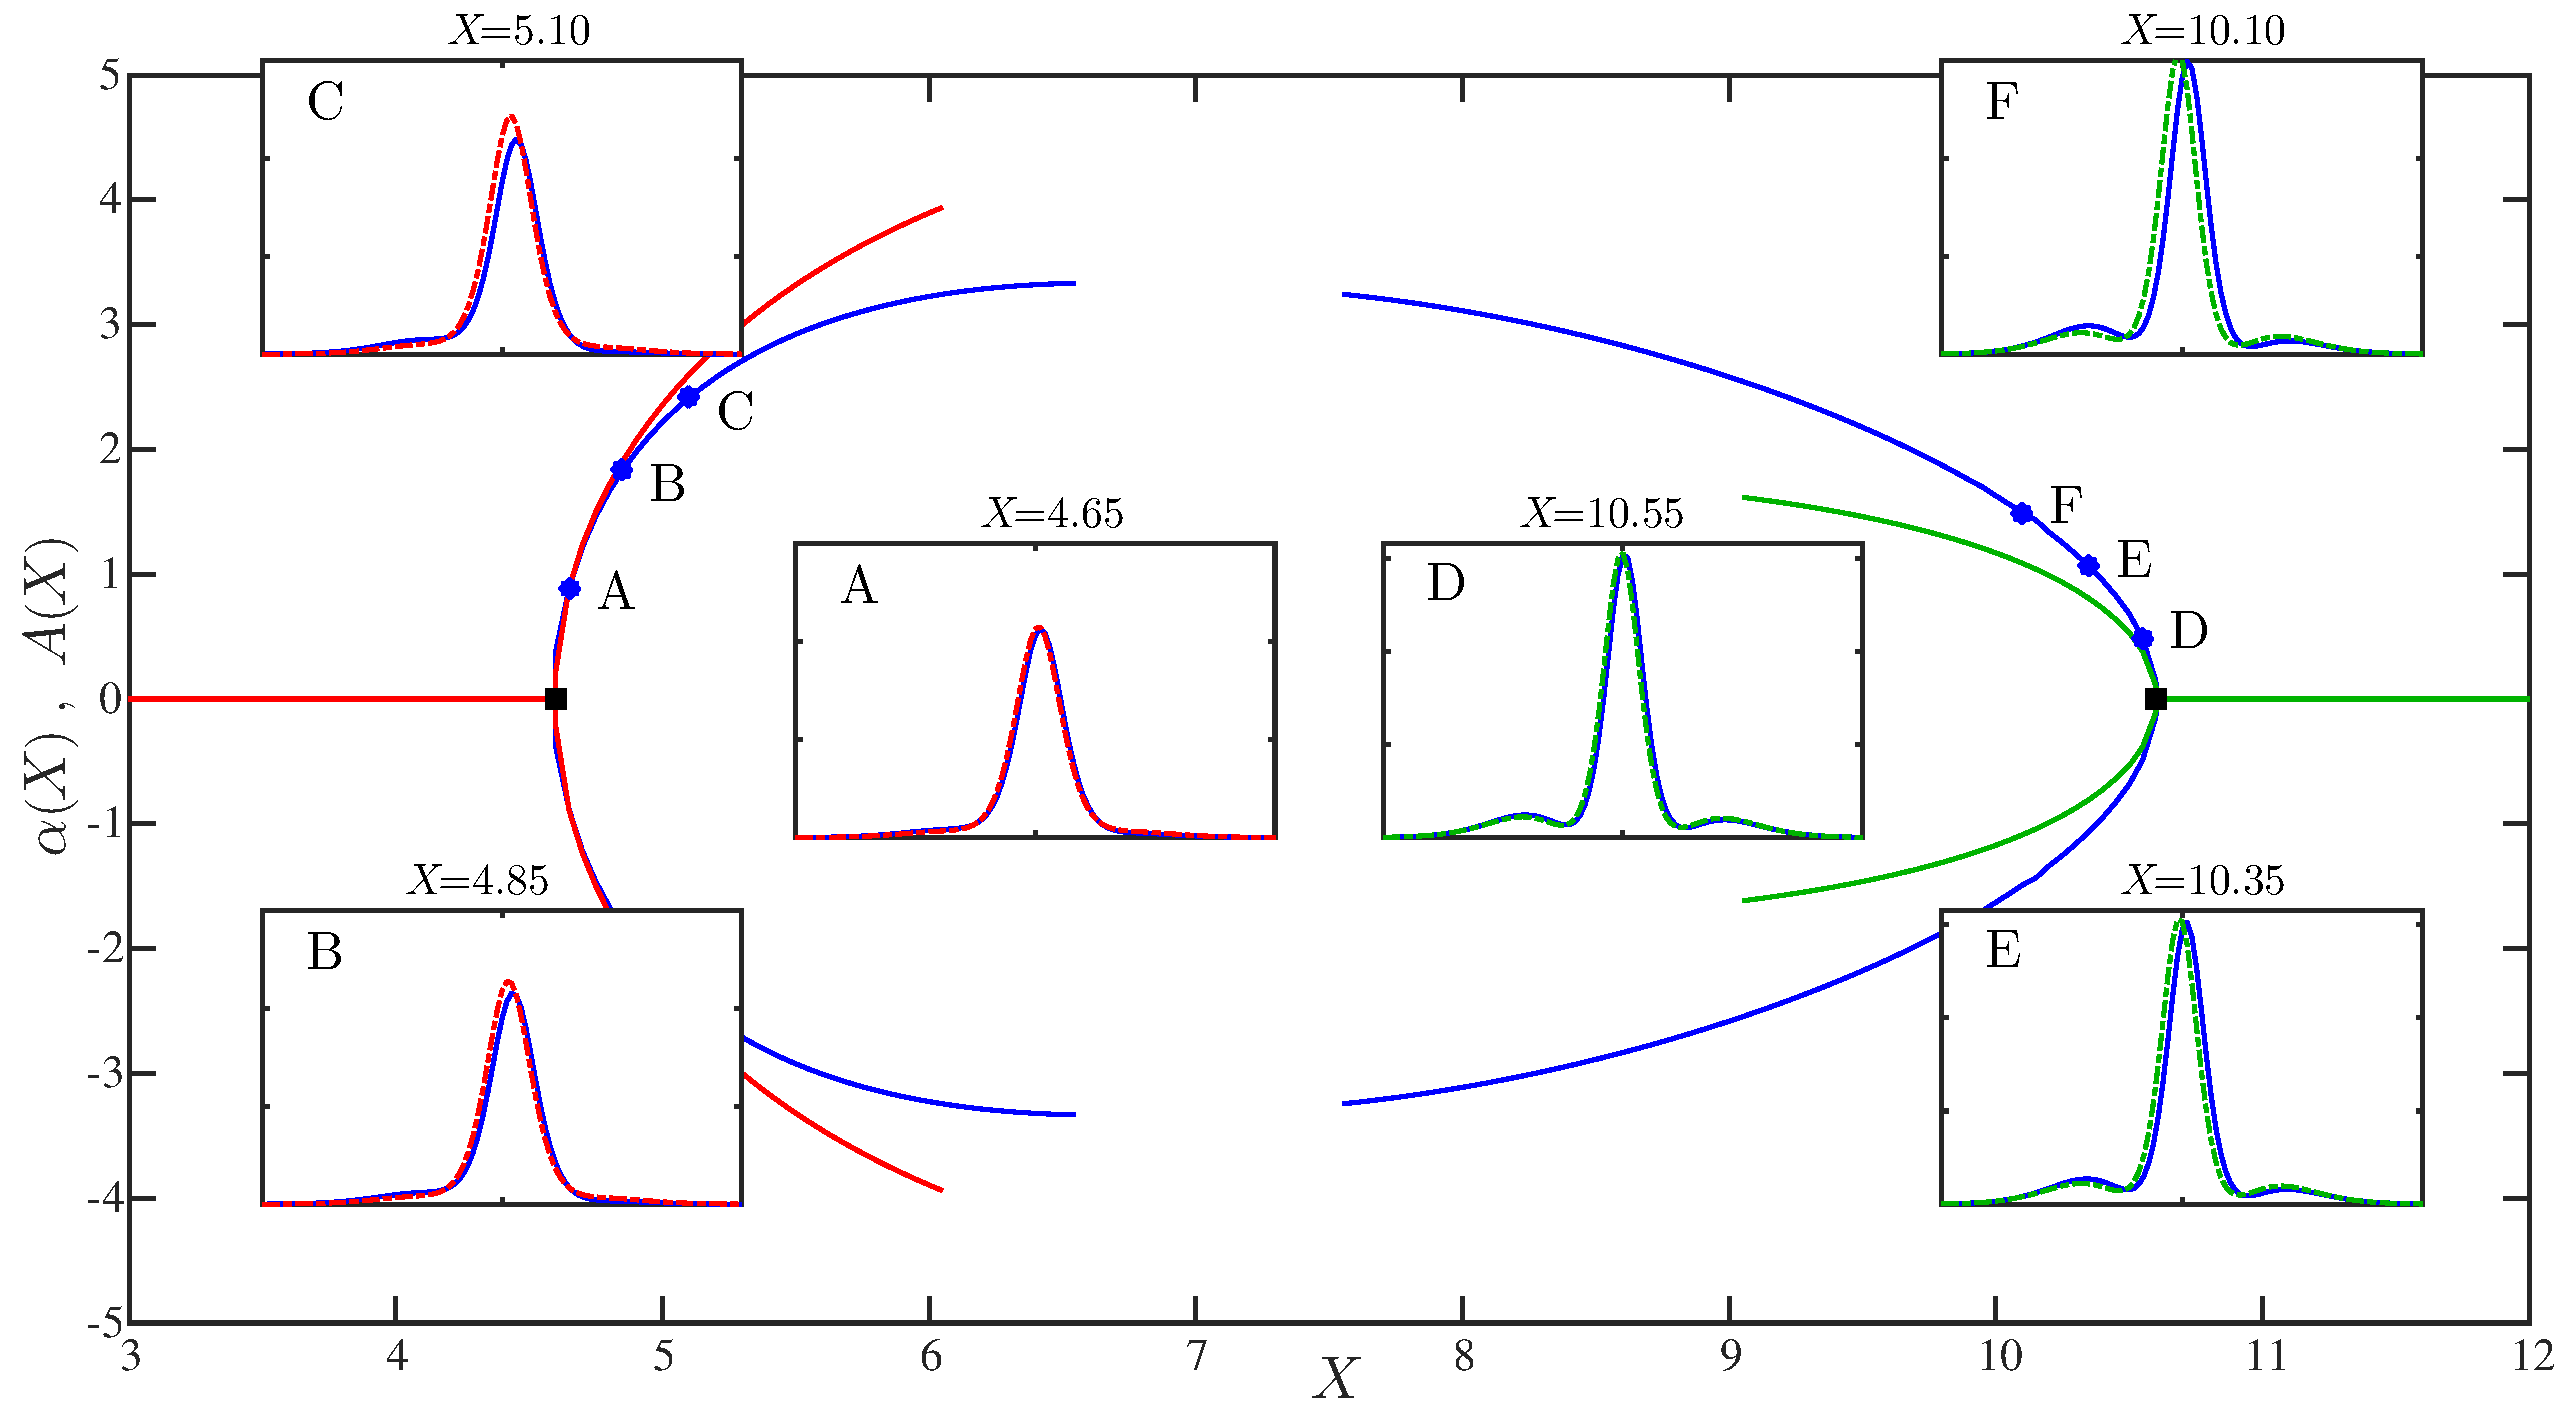
\includegraphics[width=0.8\textwidth]{PitchforkComparisonN.eps}
\caption{Coefficients determining the amount of asymmetry 
for the LL model $\alpha(X)$ and for the center manifold approach $A(X)$}
\end{figure}
\end{frame}

%Slide 31
\begin{frame}[c]{Applications: SSB}{First Pitchfork Bifurcation Orbits}
\begin{figure}[h]
\centering
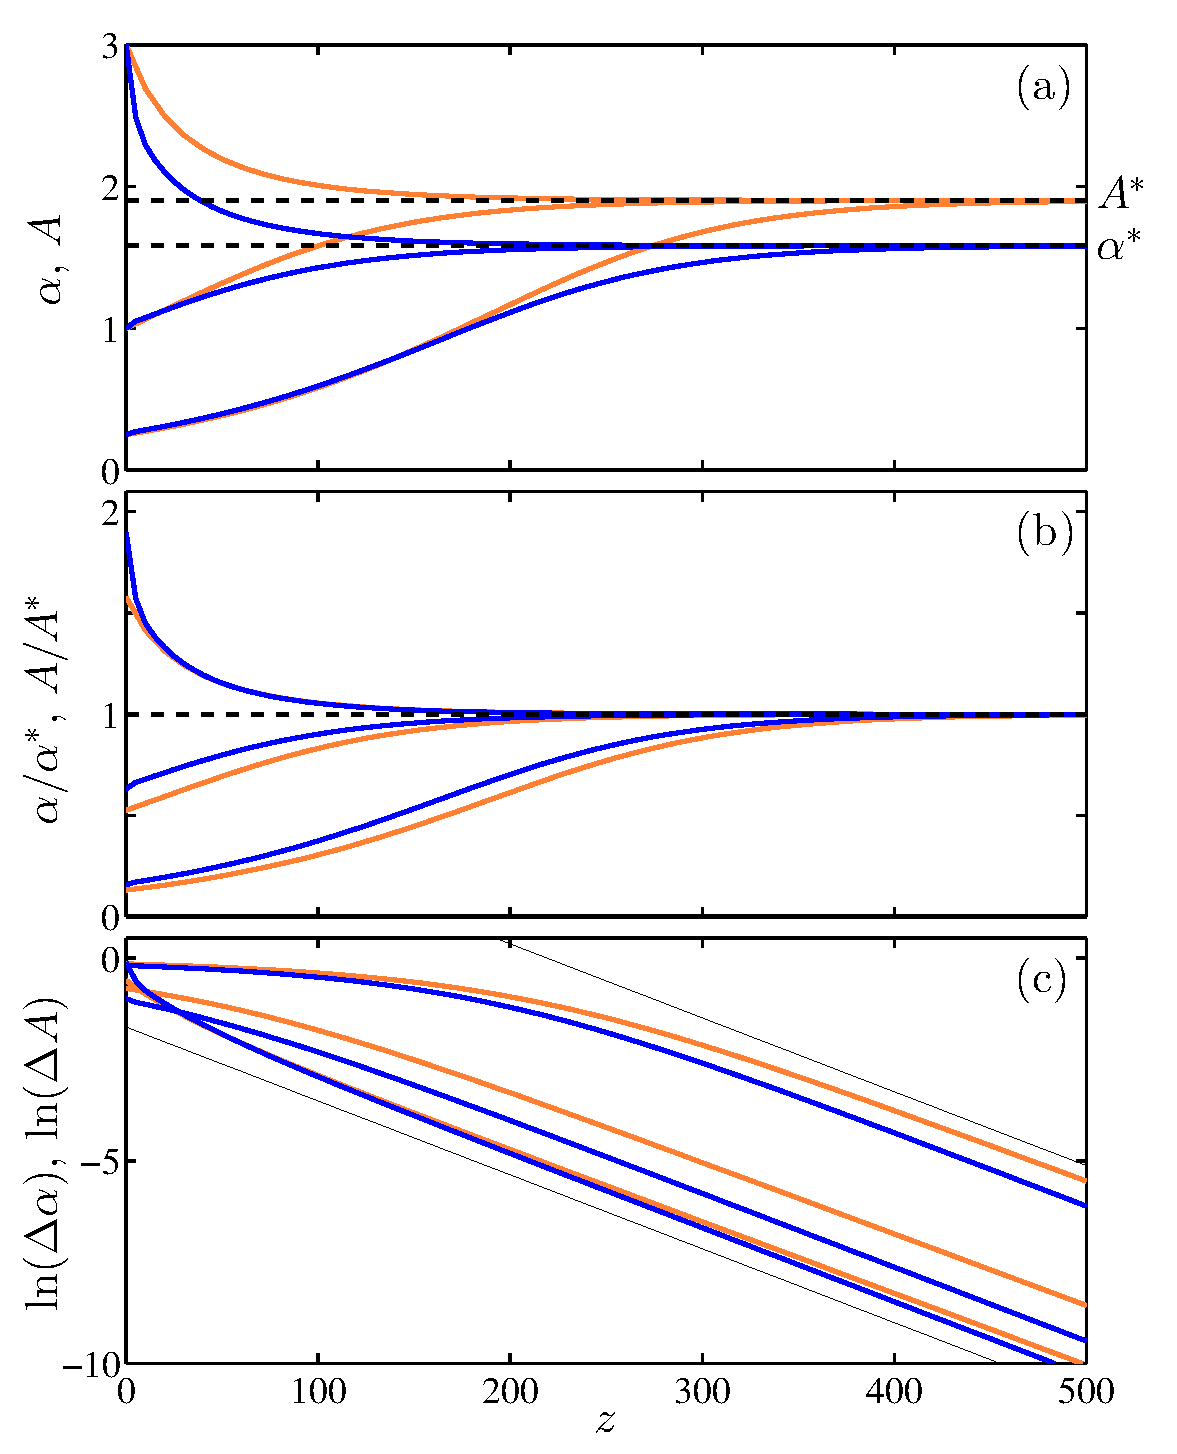
\includegraphics[height=0.6\textheight]{PitchforkPhasePortraitN.eps}
\caption{Orbits representing the dynamics settling to the
asymmetric steady states past the first pitchfork bifurcation point for $X=4.85$. 
The logarithm of the normalized distance to the
steady state are $\Delta \alpha=(\alpha-\alpha^*)/\alpha^*$ 
and $\Delta A=(A-A^*)/A^*$.  In this panel we also depict with thin (black) lines the slope 
$\lambda(4.85)=-0.01824$ corresponding 
to the stability eigenvalue of the asymmetric state.
}
\end{figure}
\end{frame}


\begin{frame}[c]{Applications: Temporal Tweezing of Light}{\textcolor{paleblue}{Motivation} }
\begin{block}{\small{Mean-field Lugiato-Lefever equation for Cavity Solitons}}
\tiny{\[ 
t_R \frac{\partial F(z,\tau)}{\partial z} - \beta_2 L \phi' \frac{\partial F}{\partial \tau} = \left[ -\alpha_F - i \delta_F - i L \frac{\beta_2}{2} \frac{\partial^2}{\partial \tau^2} + i \gamma L |F|^2 \right] F + \sqrt{\theta} F_{\mathrm{in}} 
\] }
\end{block}
\begin{figure}[H!]
\centering
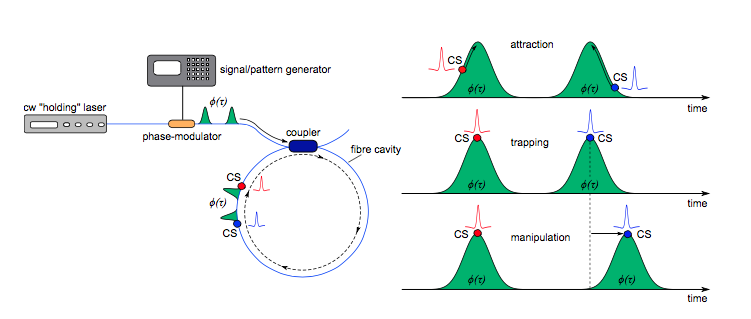
\includegraphics[width=0.7\textwidth, height=2.5cm]{TemporalTweeze.png} \\
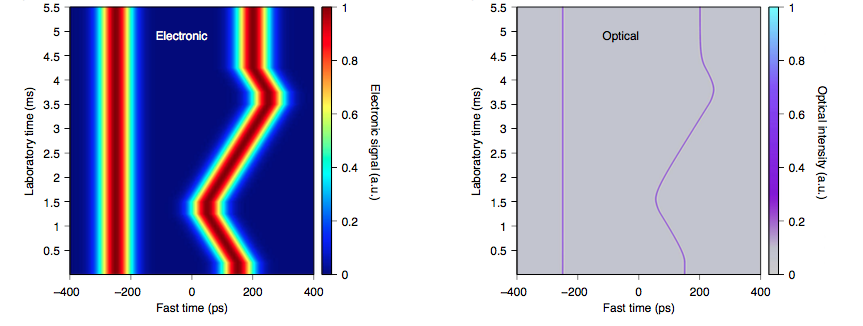
\includegraphics[width=0.5\textwidth, height=2.4cm]{ResultsTweeze.png}
\caption{\tiny{\fullcite{tweeze}}}
\end{figure}

\end{frame}

\begin{frame}[c]{Applications: Temporal Tweezing of Light}{Dimensionless Mean-field Lugiato-Lefever Equation }
   \tikz[baseline=-.5ex]\node[fill=Comment,anchor=north, rounded corners] (nlsnote2) {
	\textcolor{white}{NLS}
	};   \quad \quad 
	\hspace{2em}\tikz[baseline=-.5ex]\node[fill=turtlegreen,anchor=north, rounded corners] (phasenote) {
	\textcolor{white}{Cavity phase detuning}
	};

\vspace{1.5em}

%\end{itemize}
\begin{align*}
        \tikz[baseline=-.5ex]{
            \node (nls) {\textcolor{Comment}%[fill=blue!20,anchor=base] (t1)
            {$ i v_z +  v_{\tau\tau} + |v|^2 v $}};
        }  -
        \tikz[baseline=-.5ex]{
	\node (phase) {\textcolor{turtlegreen}
            {$\Delta v$}};
        } =  -
        \tikz[baseline=-.5ex]{
            \node (lossi) {\textcolor{paleblue}
            {$ i v$}} ;
        } +
         \tikz[baseline=-.5ex]{
	\node (gainS) {\textcolor{crimsonred}
            {$i v_{\mathrm{in}}$}};
        }.
\end{align*}

\vspace{1.5em}
	
	\hspace{4em}\tikz[baseline=-.5ex]\node[fill=paleblue,anchor=north, rounded corners] (lossinote) {
	\textcolor{white}{Cavity losses}
	};  \quad \quad
	\hspace{4em}\tikz[baseline=-.5ex]\node[fill=crimsonred,anchor=north, rounded corners] (gainSnote) {
	\textcolor{white}{Holding beam}
	};

   	\begin{tikzpicture}[overlay, line width=1.5]
	        \path[->,color=Comment] (nlsnote2) edge [bend left] (nls);
	        \path[->,color=turtlegreen] (phasenote) edge [bend left] (phase);
	        	\path[->,color=paleblue] (lossinote) edge [bend right] (lossi);
		\path[->,color=crimsonred] (gainSnote) edge [out=0, in=245] (gainS);
	        % \path[->]<2-> (n2) edge [bend right] (t2);
	        % \path[->]<3-> (n3) edge [out=0, in=-90] (t3);
	\end{tikzpicture}
	
 \textcolor{regal}{Steady state solution: 
 \begin{align*} 
 v_s = \frac{ v_{\mathrm{in}} }{1 + i(\Delta - |v_s|^2)} 
 \end{align*} 
 } 

\end{frame}

\begin{frame}[c]{Applications: Temporal Tweezing of Light}{LL with Phase-Modulation of the Holding Beam}
\vspace{0.5em}
\fontsize{9}{9}{Assume phase-modulation temporal profile $\phi(\tau)$, such that holding beam is 
$v_{\mathrm{in}} (\tau) = u_{\mathrm{in}} \exp[i \phi(\tau)], \label{uin}$
and use ansatz $v(z, \tau) = u(z, \tau) \exp[i \phi(\tau)]$:}
   \tikz[baseline=-.5ex]\node[fill=Comment,anchor=north, rounded corners] (nlsnote2) {
	\textcolor{white}{NLS}
	};   \quad \quad 
	\hspace{2em}\tikz[baseline=-.5ex]\node[fill=turtlegreen,anchor=north, rounded corners] (phasenote) {
	\textcolor{white}{Cavity phase detuning + Effective Potential}
	};
\vspace{1.5em}
\fontsize{9}{9}{\begin{align*}
        \tikz[baseline=-.5ex]{
            \node (nls) {\textcolor{Comment}%[fill=blue!20,anchor=base] (t1)
            {$ i u_z +  u_{\tau\tau} + |u|^2 u $}};
        }  -
        \tikz[baseline=-.5ex]{
	\node (phase) {\textcolor{turtlegreen}
            {$(\Delta + (\phi')^2) u$}};
        } +
        \tikz[baseline=-.5ex]{
	\node (drift) {\textcolor{regal}
            {$2 i u_{\tau} \phi' $}};
        } =  -
        \tikz[baseline=-.5ex]{
            \node (lossi) {\textcolor{paleblue}
            {$ i (1+\phi'') u$}} ;
        } +
         \tikz[baseline=-.5ex]{
	\node (gainS) {\textcolor{crimsonred}
            {$i u_{\mathrm{in}}$}};
        }.
\end{align*}}
\vspace{1.5em}	
	\hspace{2em}\tikz[baseline=-.5ex]\node[fill=regal,anchor=north, rounded corners] (driftnote) {
	\textcolor{white}{Drift with speed $2 \phi'$}
	};  \quad \quad
	\hspace{2em}\tikz[baseline=-.5ex]\node[fill=paleblue,anchor=north, rounded corners] (lossinote) {
	\textcolor{white}{Cavity losses}
	};  \quad \quad
	\hspace{2em}\tikz[baseline=-.5ex]\node[fill=crimsonred,anchor=north, rounded corners] (gainSnote) {
	\textcolor{white}{Holding beam}
	};
   	\begin{tikzpicture}[overlay, line width=1.5]
	        \path[->,color=Comment] (nlsnote2) edge [bend left] (nls);
	        \path[->,color=turtlegreen] (phasenote) edge [bend left] (phase);
	        \path[->,color=regal] (driftnote) edge [bend right] (drift);
	        	\path[->,color=paleblue] (lossinote) edge [bend right] (lossi);
		\path[->,color=crimsonred] (gainSnote) edge [out=0, in=245] (gainS);
	        % \path[->]<2-> (n2) edge [bend right] (t2);
	        % \path[->]<3-> (n3) edge [out=0, in=-90] (t3);
	\end{tikzpicture}
\end{frame}

%Slide 
\begin{frame}[c]{Applications: Temporal Tweezing of Light}{Tweezability of Cavity Solitons}
\begin{columns}
\begin{column}{0.8\textwidth}
\fontsize{8}{8}{\begin{itemize}
\item Assume Gaussian phase profile 
\fontsize{7}{7}{
\[\phi(\tau) = h_{\phi} \exp\left[ -\frac{(\tau - \tau_0)^2}{2 \sigma_{\phi}^2} \right],  \quad \phi' = -\frac{h_{\phi}(\tau - \tau_0)}{\sigma_{\phi}^2} \exp\left[ -\frac{(\tau - \tau_0)^2}{2 \sigma_{\phi}^2} \right],\]
\[\phi'' =- \frac{h_{\phi}}{\sigma_{\phi}^2}\left(1+\frac{(\tau - \tau_0)^2}{\sigma_{\phi}^2} \right) \exp\left[ -\frac{(\tau - \tau_0)^2}{2 \sigma_{\phi}^2} \right].\]
}
\fontsize{8}{8}{\item Effective Potential = \textcolor{paleblue}{Tweezer} (\textcolor{paleblue}{$(\phi')^2$})}
%\item Stationary Solutions 
%\begin{align*}
% u_{0,\tau\tau}  + \left( |u_0|^2 -\Delta -  (\phi')^2 \right) u_0 + 2 i \phi' u_{0, \tau}=  - i (1+\phi'')  u_0 + i u_{\mathrm{in}},
%\end{align*}
%with power-balance constraint ($dP/dz= 0$, where total power $P \equiv \int_{-\infty}^{\infty} |u|^2 d \tau$)
%\begin{align*}
%\int_{-\infty}^{\infty} \left [ - (1 + \phi'') |u_0|^2 - \phi' \left( u_{0,\tau} u_0^* + u_{0,\tau}^*u_0 \right) + \mathrm{Re}(u_0) u_{\mathrm{in}} \right ] d \tau = 0.
%\end{align*}
\fontsize{8}{8}{\item Simulate moving and manipulation through phase-profile }
\fontsize{7}{7}{
\[\tau_0 (z) = \frac{\tau_f}{2} \left [ \frac{1}{\mathrm{tanh} (\beta z^*)} \mathrm{tanh} [\beta (z - z^*)] + 1\right],\] }
\fontsize{8}{8}{ \hskip -0.5em where $z^*$ is the total slow time to reach $\tau_f$ -- the final $\tau$ -- and $\beta$ is the adiabaticity parameter, which together describe the speed of the effective potential. }
\end{itemize}}
\end{column}
\begin{column}{0.3\textwidth}
\centering
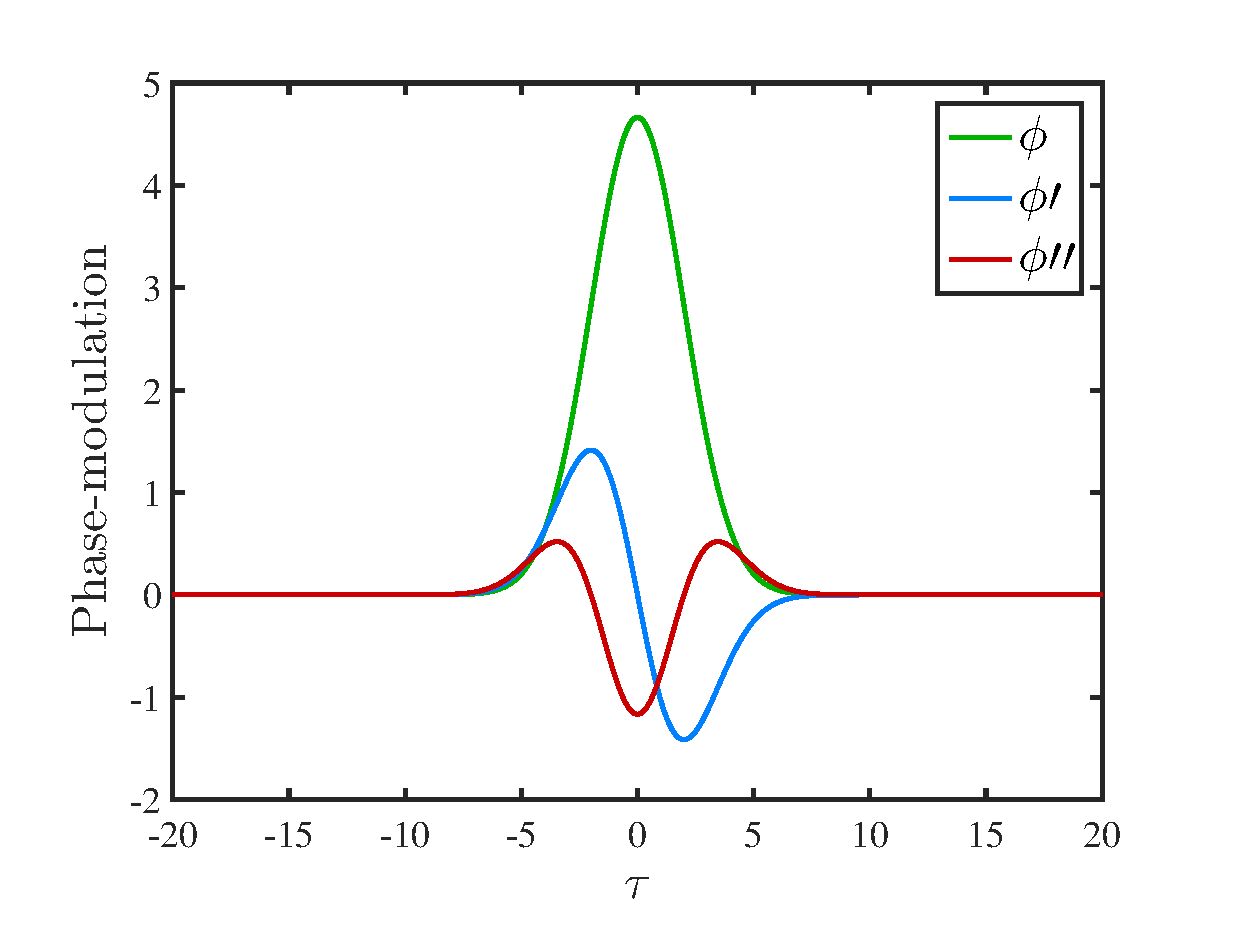
\includegraphics[height = 0.28\textheight]{phase.eps}\\
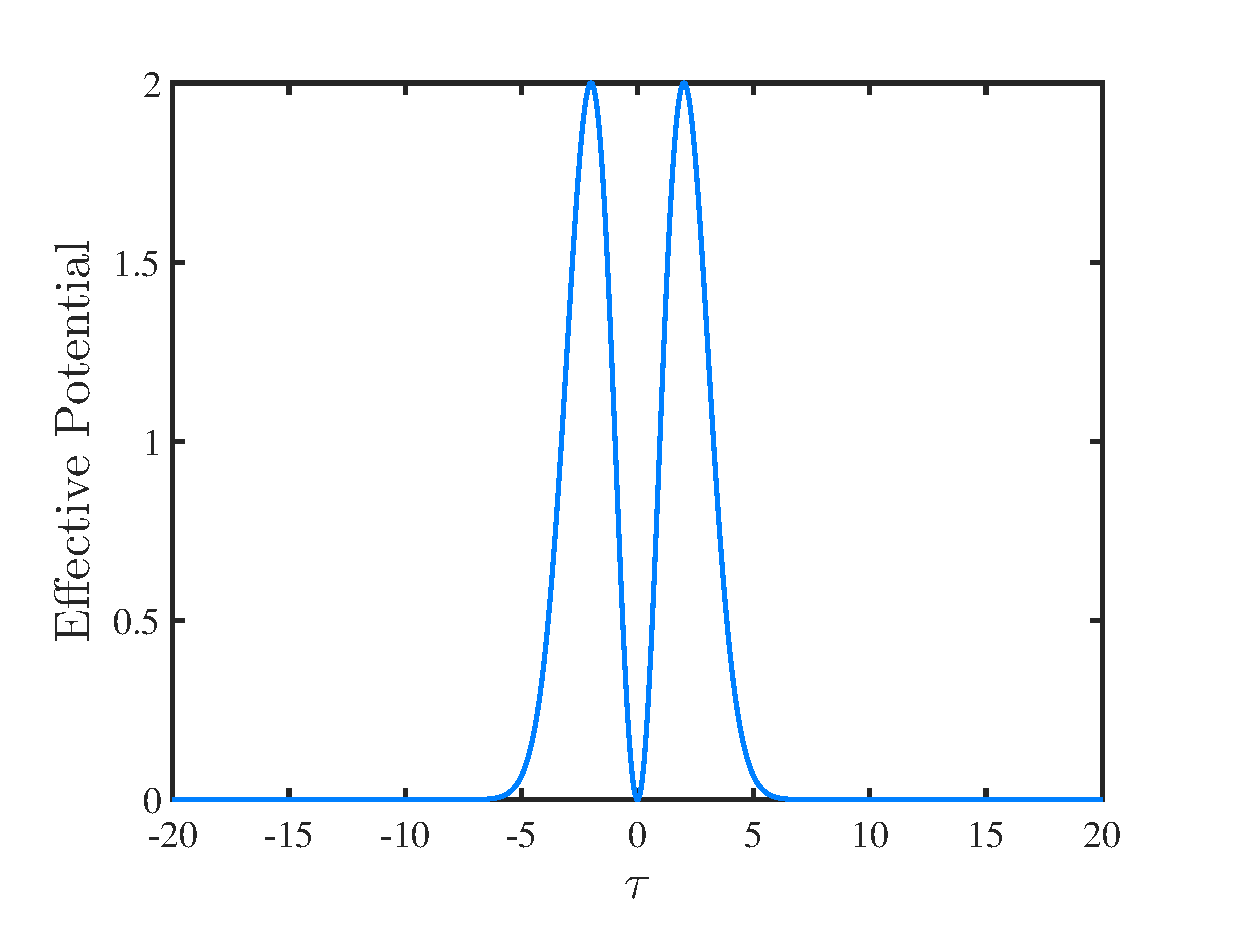
\includegraphics[height = 0.28\textheight]{phase_pot.eps}\\
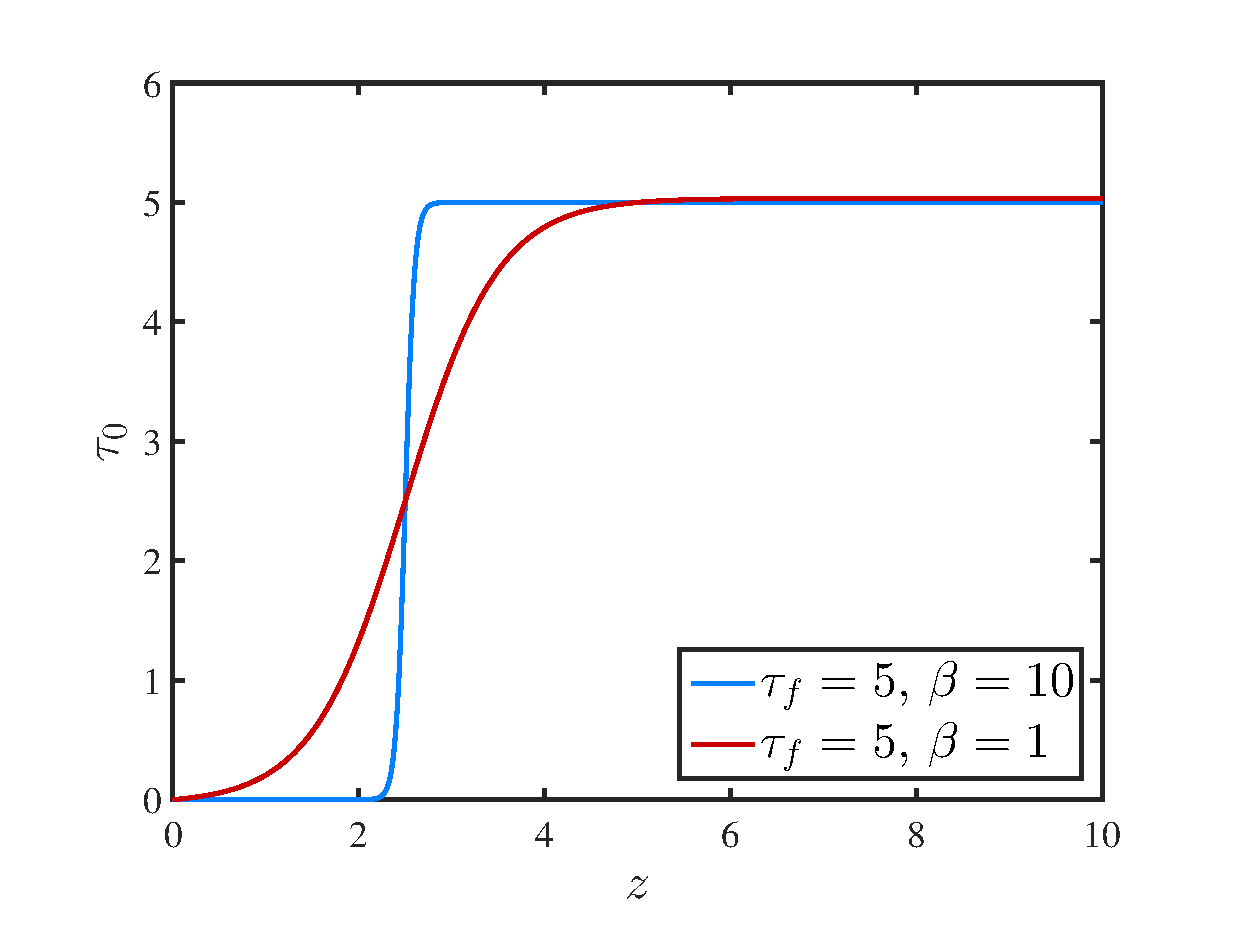
\includegraphics[height = 0.28\textheight]{phase_pot2.eps}
\end{column}
\end{columns}
\end{frame}

%Slide
\begin{frame}[c]{Applications: Temporal Tweezing of Light}{Dynamical States of Cavity Solitons and Tweezers}
\begin{columns}
\begin{column}{0.5\textwidth}
\begin{figure}[H]
\centering
\centerline{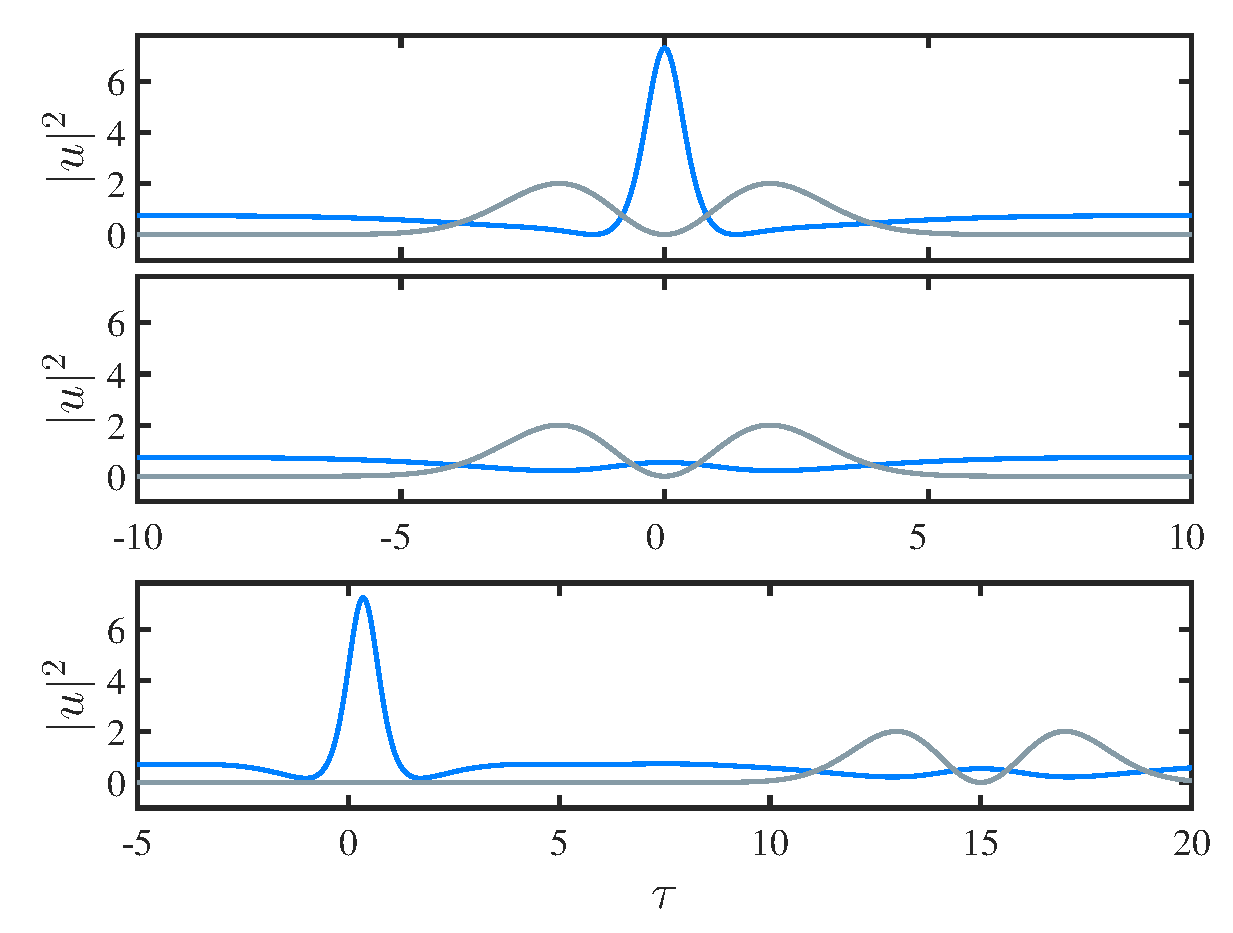
\includegraphics[width=0.9\textwidth]{threeStates.eps}}
\caption{Temporal Profiles of Fundamental States:  Tweezed CS, no-CS, and non-tweezed CS}
\end{figure}
\end{column}
\begin{column}{0.3\textwidth}
\begin{figure}[p!]
\centering
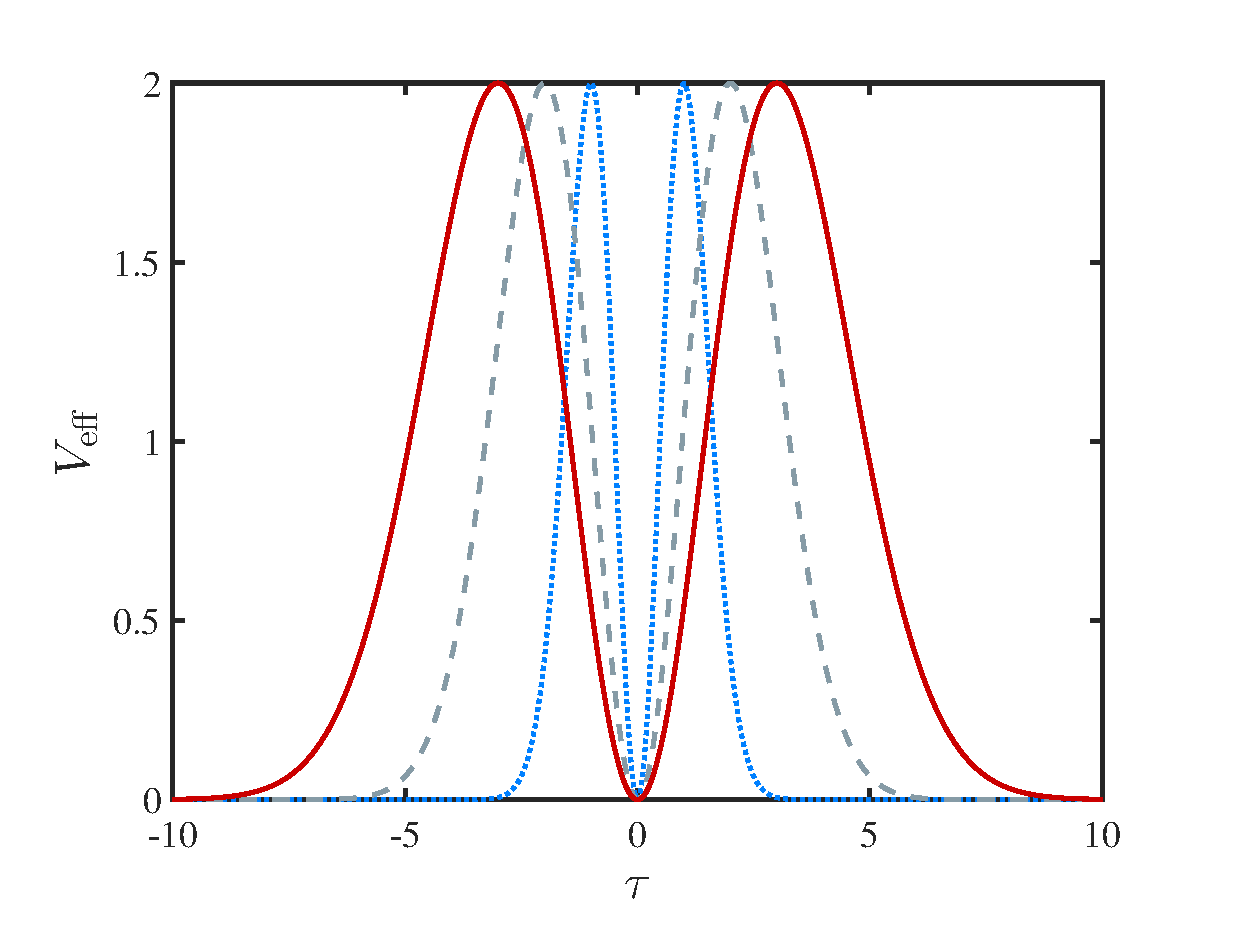
\includegraphics[width=0.8\textwidth]{potentials.eps}\\
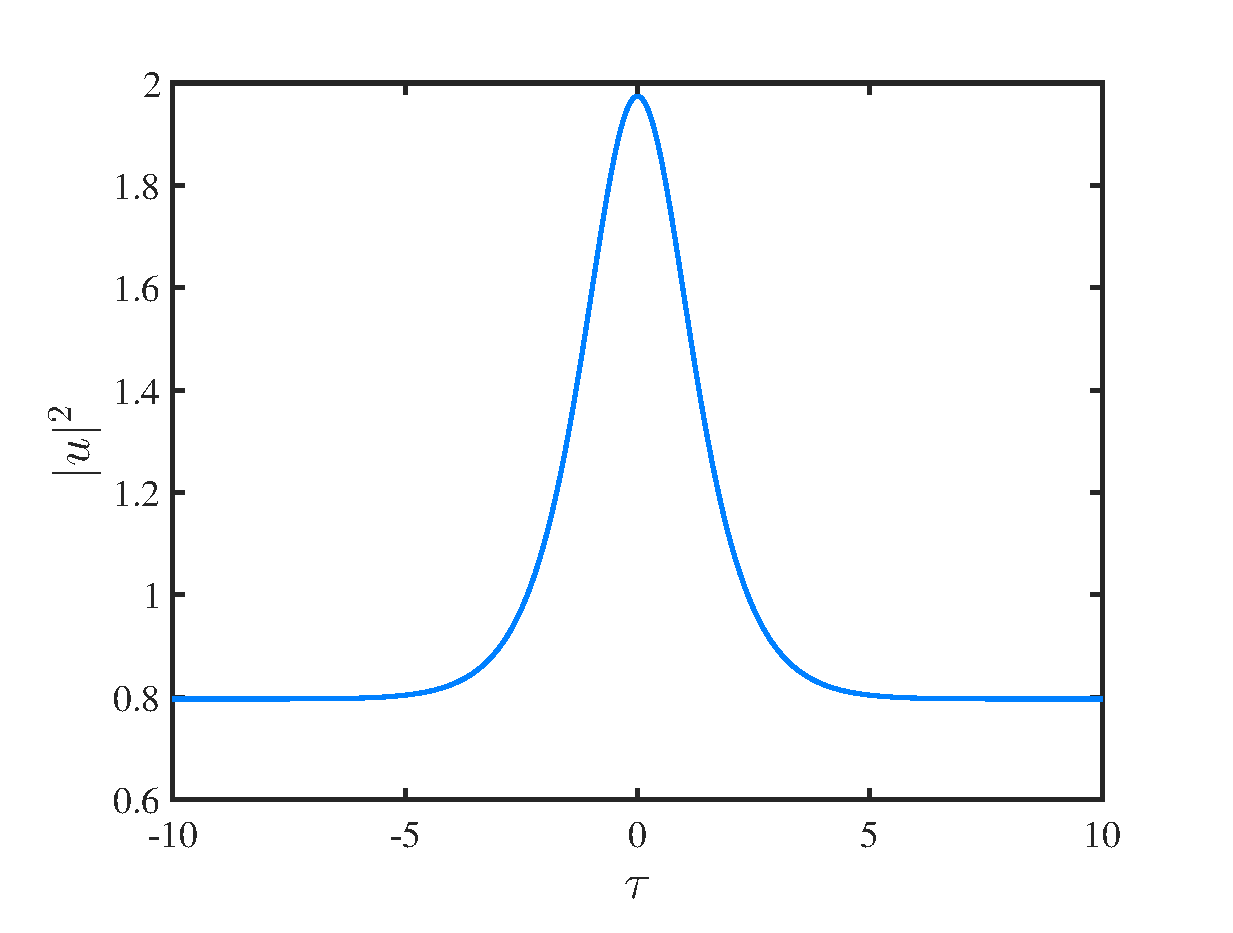
\includegraphics[width=0.8\textwidth]{noTrapCS.eps}
\caption{ \textcolor{paleblue}{Tweezers} ($V_{\mathrm{eff}} = (\phi')^2$) of Narrow ($\sigma_\phi = 1$), Natural ($\sigma_\phi = 2$), 
and Wide ($\sigma_\phi = 3$) Widths.
}
\end{figure}
\end{column}
\end{columns}
\end{frame}

%Slide 
\begin{frame}[c]{Applications: Temporal Tweezing of Light}{NCVA}
\fontsize{9}{9}{ \begin{itemize}
\item Construct $u = v + \bar{u}$ where $v$ is homogeneous steady-state and $\bar{u}$ is NCVA ansatz.
\item Modified LL model 
\begin{align*}
i \bar{u}_z + |\bar{u}|^2 \bar{u} + \bar{u}_{\tau\tau} & - (\Delta + (\phi')^2 -2|v|^2) \bar{u} + 2i \bar{u}_{\tau} \phi'   \\
 &= - i (1+\phi'') \bar{u} + \left((\phi')^2  - 2 |\bar{u}|^2- \phi''\right) v -  (v)^2 \bar{u}^* - (\bar{u})^2 v^*.
\end{align*}
\item  Gaussian ansatz for $j=1$ and $2$:
\begin{align*}
\bar{u}_j = a_j \exp \left[ -\frac{(\tau - \xi_j)^2}{2\sigma_j^2} \right] \exp \left[ i (d_j (\tau - \xi_j)^2 + c_j (\tau - \xi_j) + b_j ) \right]. 
\end{align*} 
\end{itemize}}
\begin{block}{\small{Non-conservative Lagrangian density}}
\vspace{-0.5em}
\fontsize{5}{5}{\begin{align*}
\bar{\mathcal{L}} =&  \frac{i}{2} \left(\bar{u}_1^* \bar{u}_{1,z} - \bar{u}_1\bar{u}_{1,z}^* \right) - |\bar{u}_{1,\tau}|^2 + \frac{1}{2} |\bar{u}_1|^4 -\left( \Delta +  (\phi')^2 -2|v|^2 \right) |\bar{u}_1|^2 + i\phi' \left(\bar{u}_1^* \bar{u}_{1,\tau} - \bar{u}_1\bar{u}_{1,\tau}^*  \right) \nonumber \\
& - \frac{i}{2} \left(\bar{u}_2^* \bar{u}_{2,z} - \bar{u}_2\bar{u}_{2,z}^* \right) + |\bar{u}_{2,\tau}|^2 - \frac{1}{2} |\bar{u}_2|^4 + \left( \Delta +  (\phi')^2 -2|v|^2 \right) |\bar{u}_2|^2 - i\phi' \left(\bar{u}_2^* \bar{u}_{2,\tau} - \bar{u}_2\bar{u}_{2,\tau}^*  \right) \nonumber \\
& + \left [ - i (1+\phi'') \bar{u}_+ + \left((\phi')^2  - 2 |\bar{u}_+|^2- \phi''\right) v -  (v)^2 \bar{u}_+^* - (\bar{u}_+)^2 v^* \right ]  \bar{u}_-,
\end{align*}}
\vspace{-0.5em}
\end{block}
\end{frame}



%Slide
\begin{frame}[c]{Applications: Temporal Tweezing of Light}{Quantifying Fundamental States}
\begin{columns}
\begin{column}{0.6\textwidth}
\fontsize{7}{7}{\begin{itemize}
\item Quantify power inside and outside tweezer with CS $\rho = |u|^2$ and no-CS $\rho_0 = |u_{\rm{no\text{-}CS}}|^2$ with  ${\rm D} = [ -\sigma_\phi, \sigma_\phi]$:
\begin{align*}
P_{\rm I}(z) = \int_{\rm D} (\rho - \rho_0) d\tau, \quad P_{\rm O}(z) = \int_{\bar{\rm D}} (\rho - \rho_0) d\tau. \label{Pout}
\end{align*} 
\item Total power 
\begin{align*}
P_{\rm Tot} = \int  (\rho - \rho_0) d\tau.
\end{align*}
\item Power ratios
\begin{align*}
Q_{\rm I} = \frac{P_{\rm I}(0) - P_{\rm I}(z_f)}{P_{\rm Tot} }, \quad Q_{\rm O}=  \frac{P_{\rm O}(0) - P_{\rm O}(z_f)}{P_{\rm Tot} }.
\end{align*}
\item Difference in power ratios:
\[  \delta Q = Q_{\rm I} - Q_{\rm O}. \]
\end{itemize}}
\end{column}
\begin{column}{0.4\textwidth}
\begin{block}{}
\fontsize{7}{7}{\small {Natural Width ($\sigma_\phi = 2$)}}
\begin{columns}
\begin{column}{0.2\linewidth}
\fontsize{8}{8}{
\hspace{0.5em} $Q_{\rm in}$ \\
\vspace{4em}
\hspace{0.4em} $Q_{\rm out}$ \\
\vspace{4em}
\hspace{0.75em} $\delta Q$
}
\end{column}
\begin{column}{0.8\linewidth}
%\begin{figure}
\centering
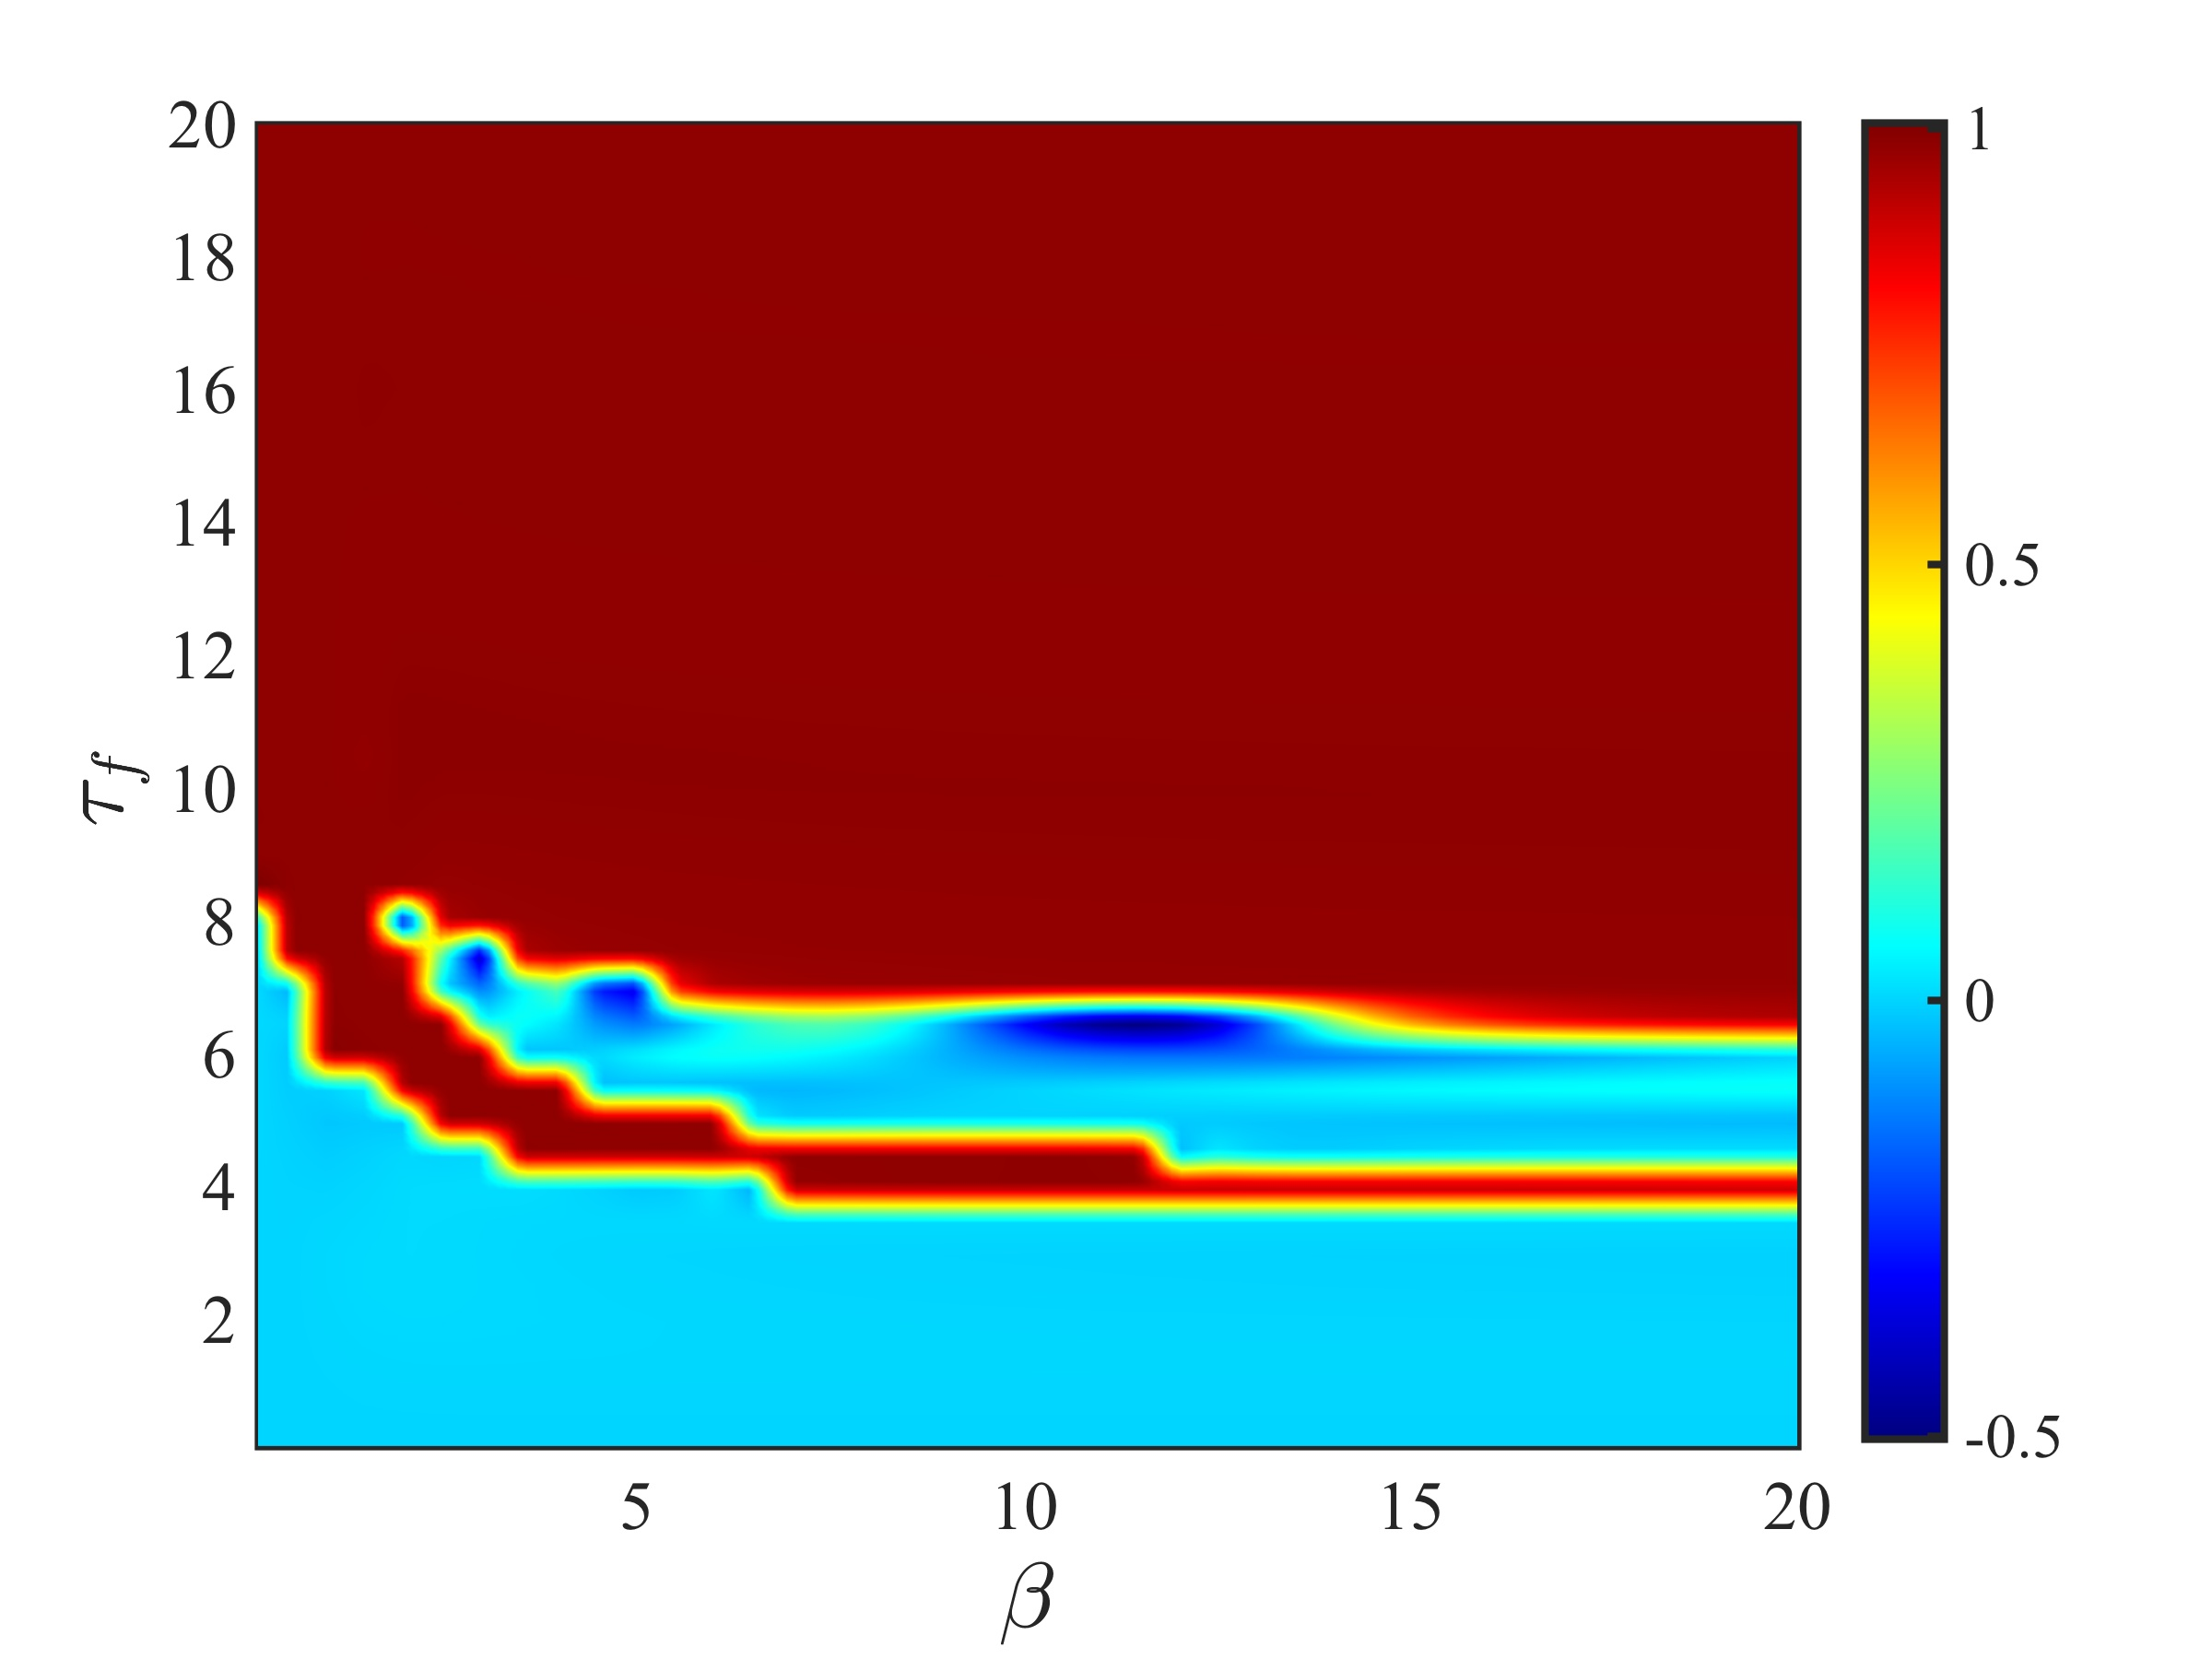
\includegraphics[height=0.25\textheight]{RegularQIn.jpg} \\
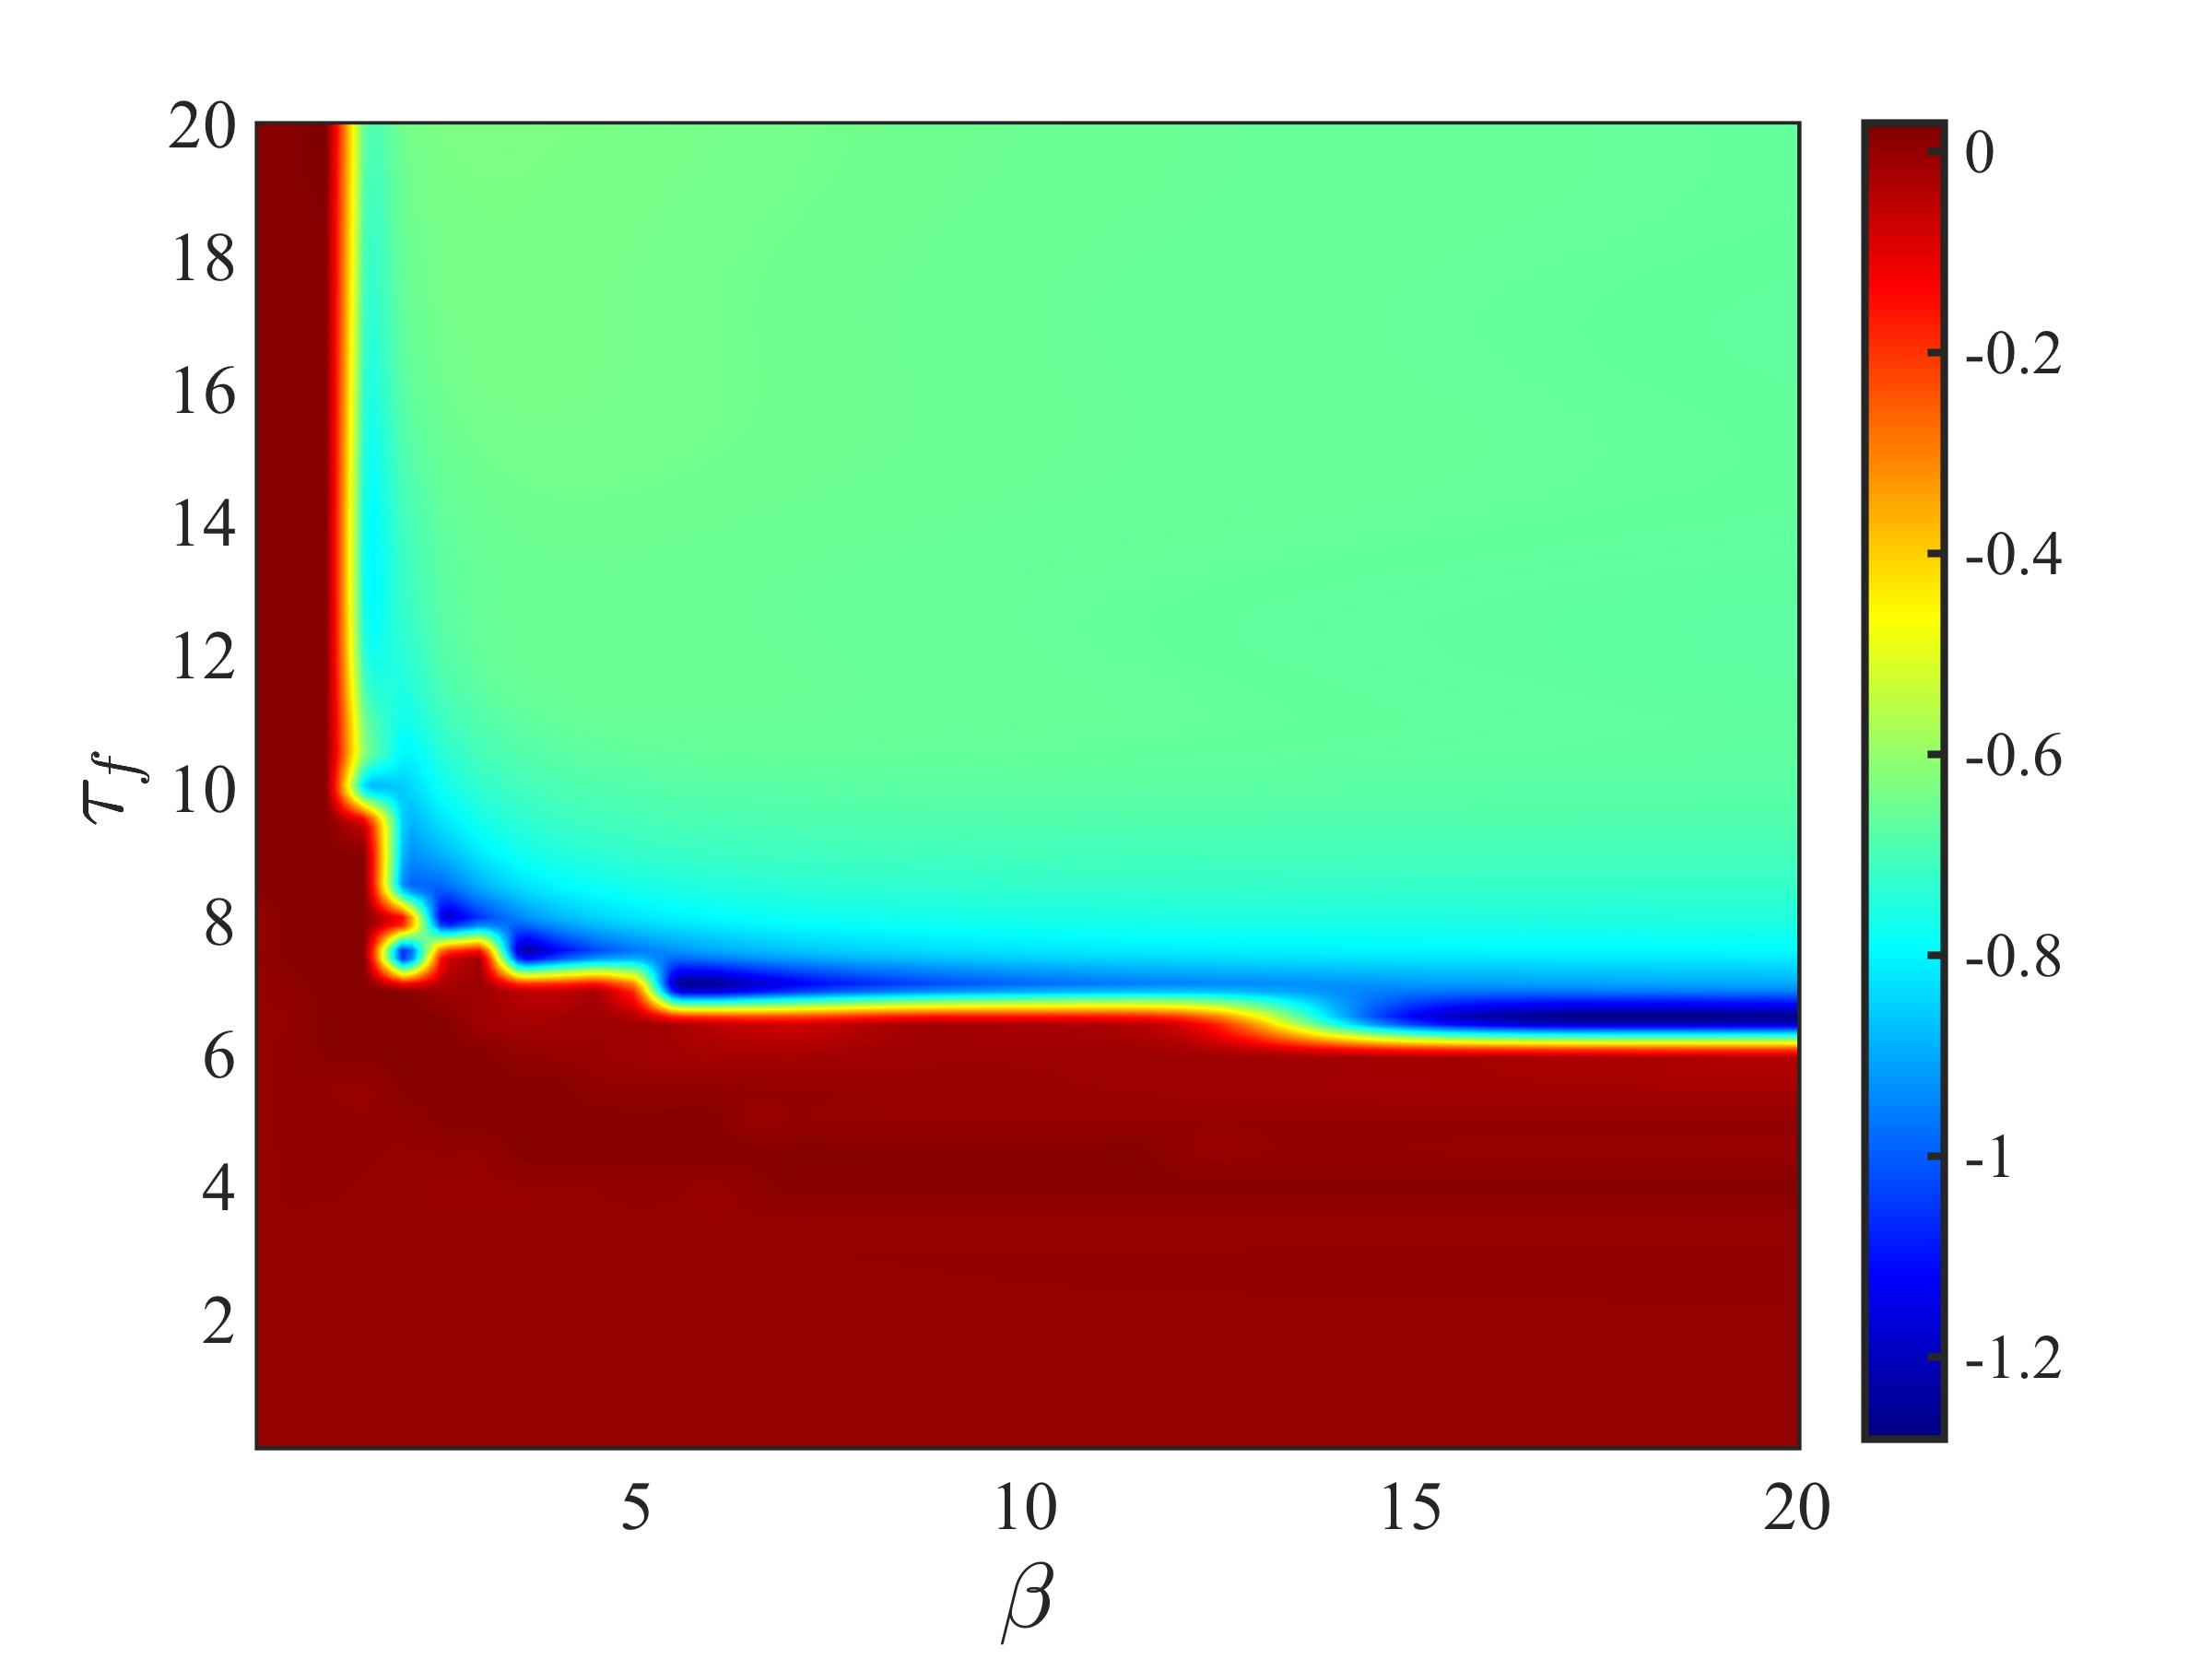
\includegraphics[height=0.25\textheight]{RegularQOut.jpg} \\
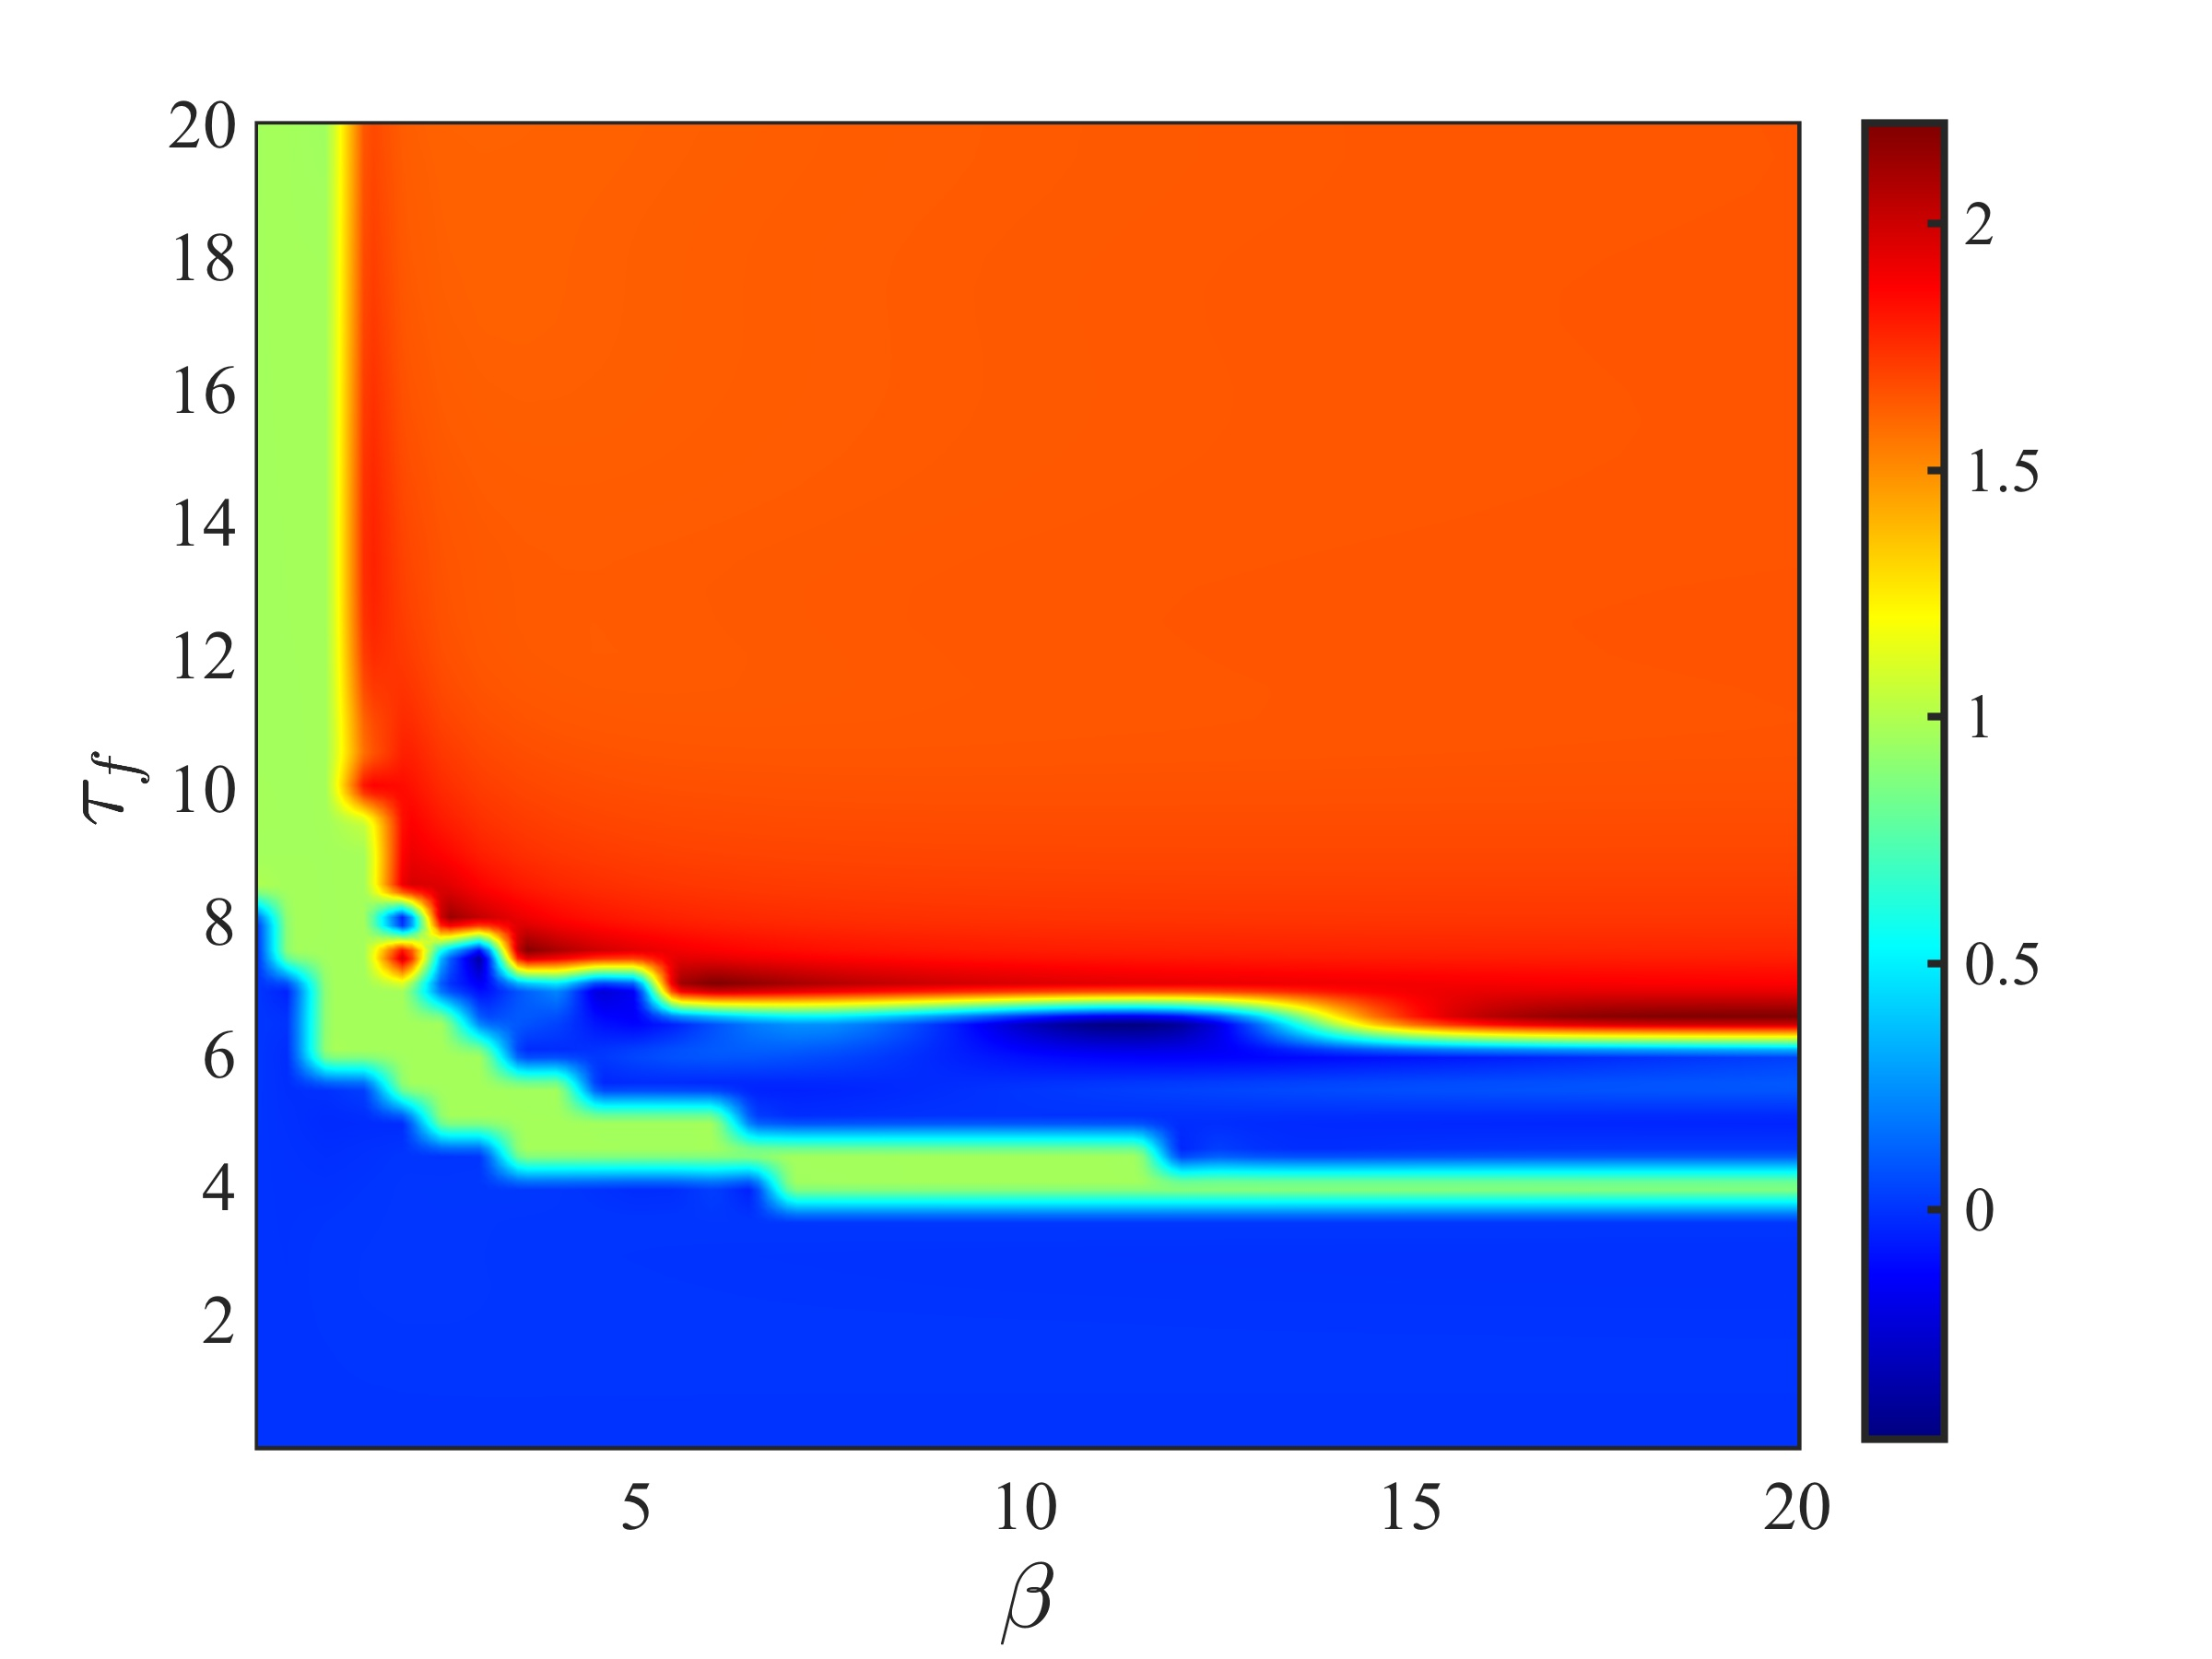
\includegraphics[height=0.25\textheight]{RegularQDiff.jpg} 
%\end{figure}
\end{column}
\end{columns}
\end{block}
\end{column}
\end{columns}
\end{frame}


%Slide  Natural
\begin{frame}[c]{Applications: Temporal Tweezing of Light}{\textcolor{paleblue}{Natural Width Tweezer} ($\sigma_\phi = 2$ and $h_\phi  = 4.6633$ )}

\begin{columns}

\begin{column}{0.28\textwidth}

\vspace{-7em}
\begin{framed}
\vspace{-1em}
\begin{figure}[h]
\centering
\centerline{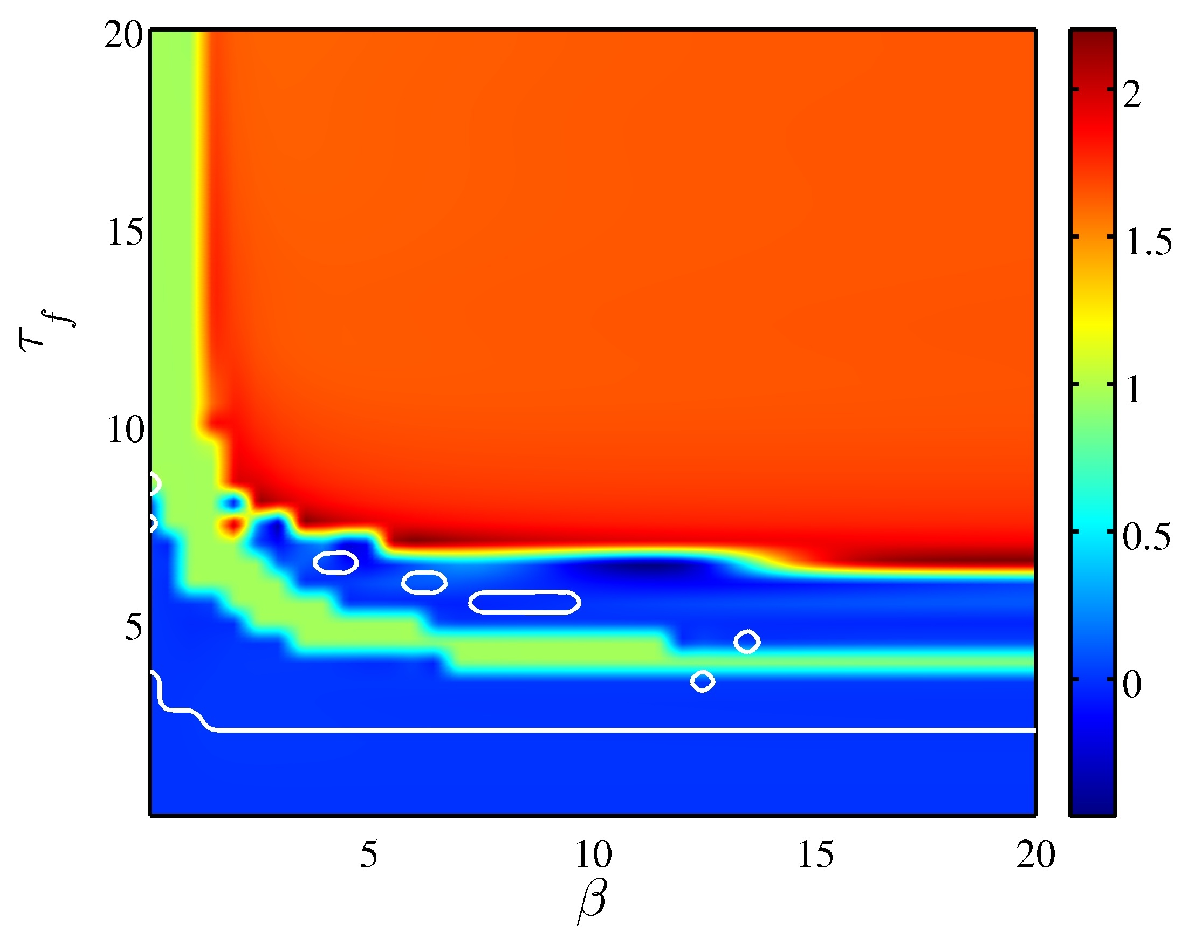
\includegraphics[width=3cm]{RegularPDEvODE_rcg_t.eps}\hspace*{0cm}}
\caption{\tiny $\delta Q$ Comparison LL Model and NCVA}
\end{figure}
\vspace{-1em}
\end{framed}
\end{column}
\vrule width 1pt

\begin{column}{0.75\textwidth}
\vspace{-0.5em}
\centering
{\small Tweezed CS:  $\tau_f =2$, $\beta = 10$ }
\vspace{0.5em}
\begin{columns}
\begin{column}{0.5\textwidth}
\vspace{-1em}
\begin{figure}
\hspace{2em}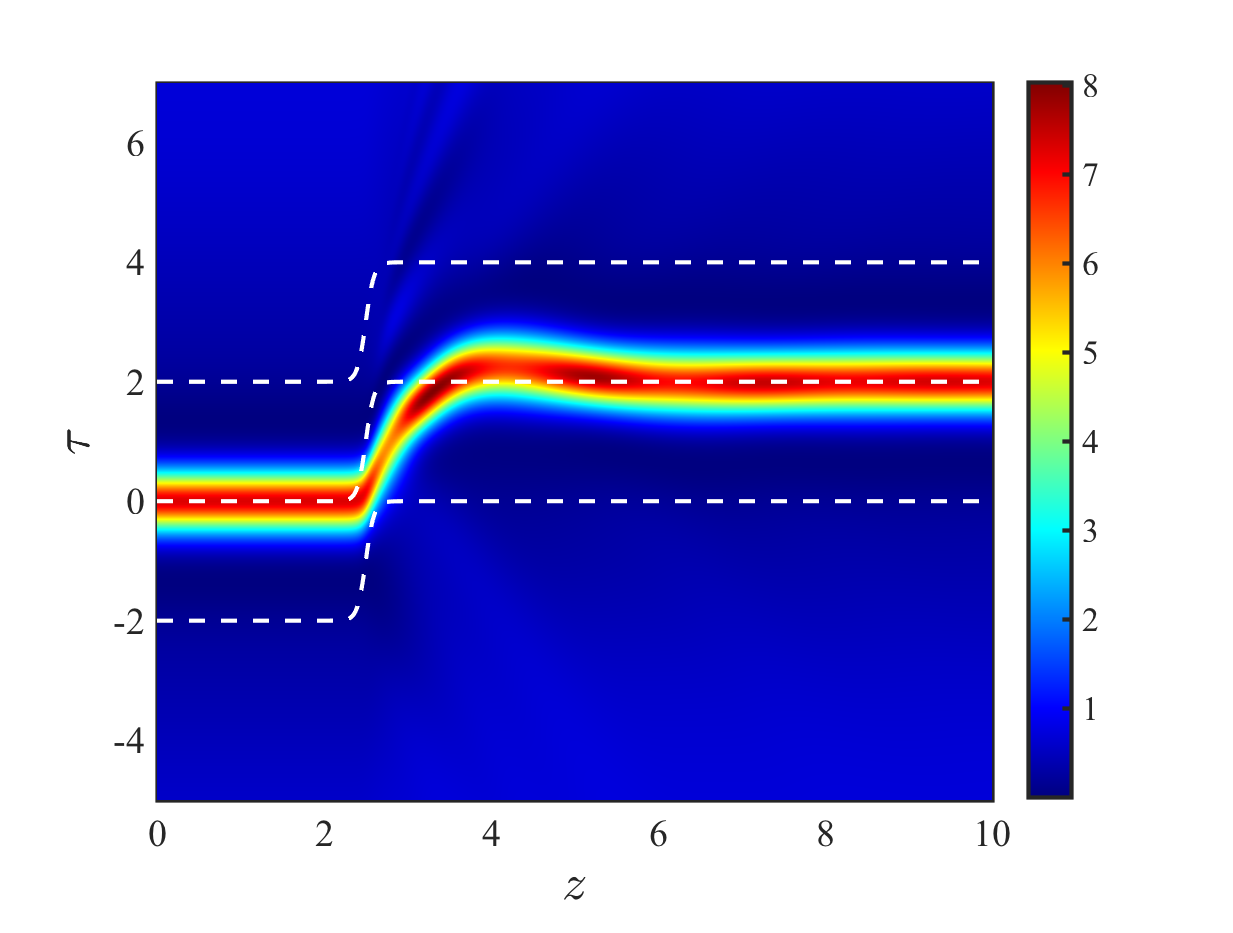
\includegraphics[width=0.5\textwidth]{regularDensity1v2.eps}  \\
\vspace{-0.5em}
\hspace{2em}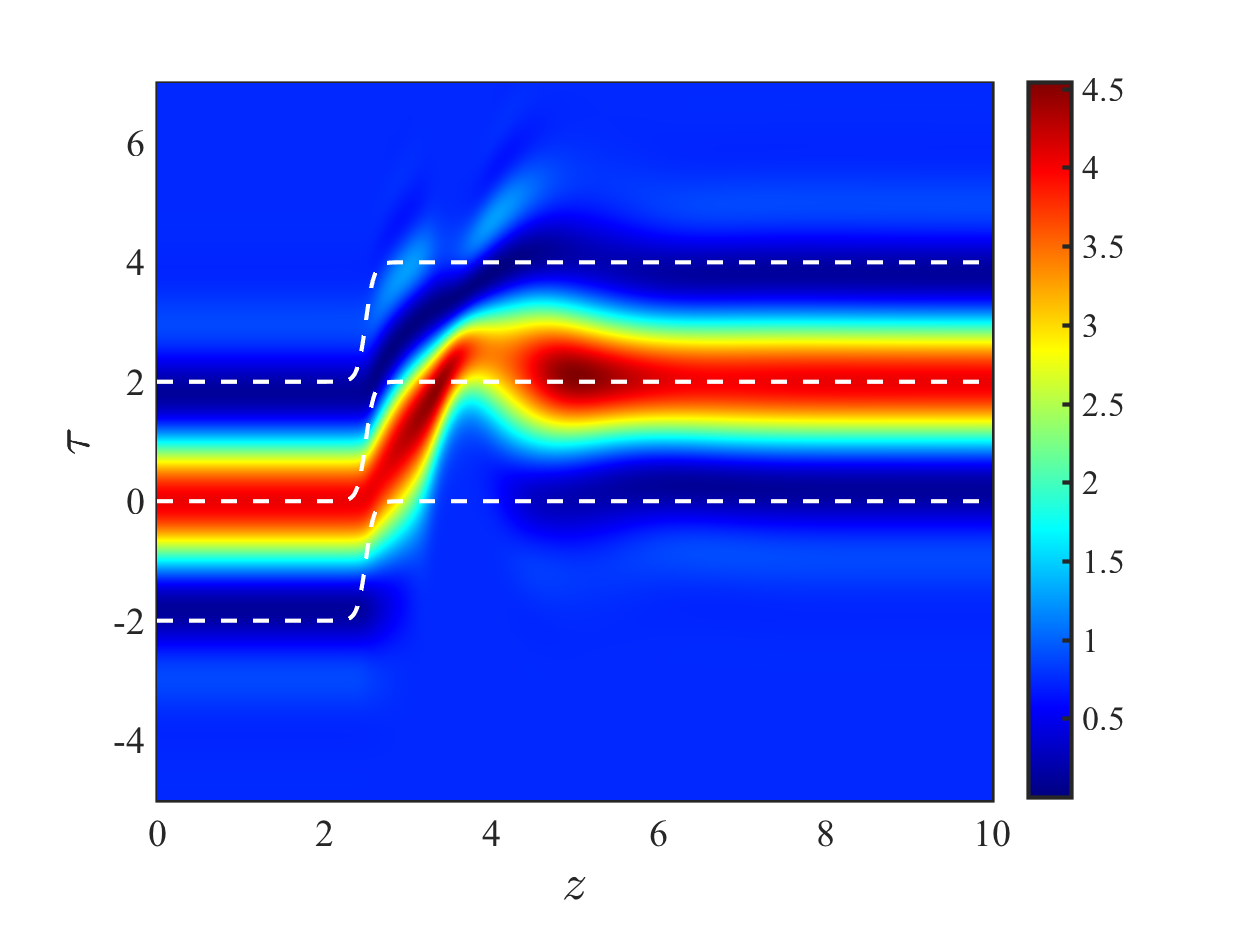
\includegraphics[width=0.5\textwidth]{regularNCVADensity1v2.eps} 
\end{figure}
\end{column}
\begin{column}{0.5\textwidth}
\vspace{-0.5em} \raggedright
\hspace{-2em}\includemedia[%
 		width=0.9\linewidth,%
		transparent=true,%
  		activate=onclick,%
		deactivate=pageclose,%
  		addresource=regular1.mp4,%
  		flashvars={source=regular1.mp4 &loop=true &controlBarAutoHide=true}%
		]{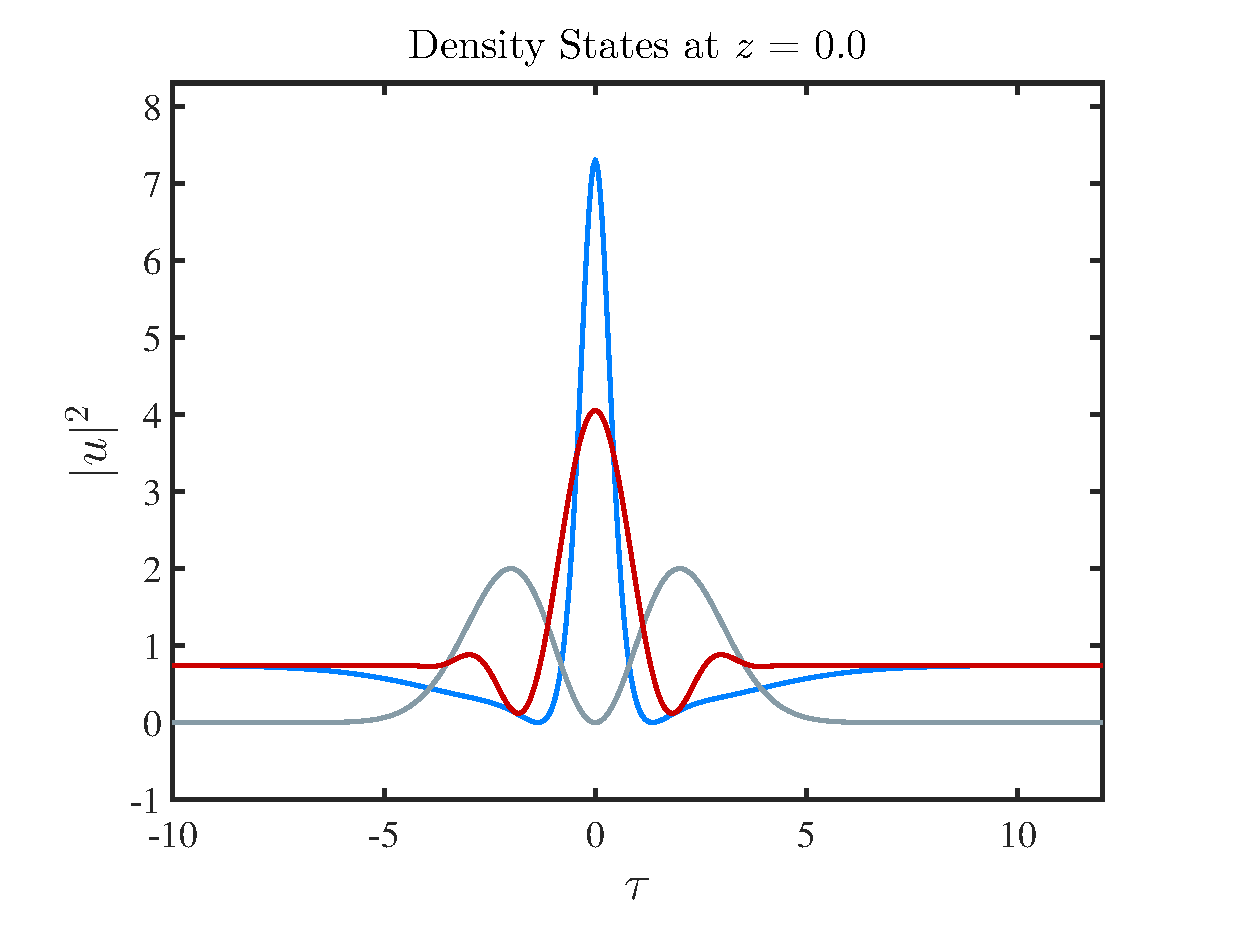
\includegraphics[width=0.5\textwidth]{regular1.eps}}{VPlayer.swf}%{StrobeMediaPlayback.swf}
\end{column}
\end{columns}
\vspace{0.5em}

\hrule width\textwidth 

\vspace{0.5em}
{\small No-CS:  $\tau_f =4.5$, $\beta = 10$ }
\begin{columns}
\begin{column}{0.5\textwidth}
\centering
\vspace{-1em}
\begin{figure}
\hspace{2em}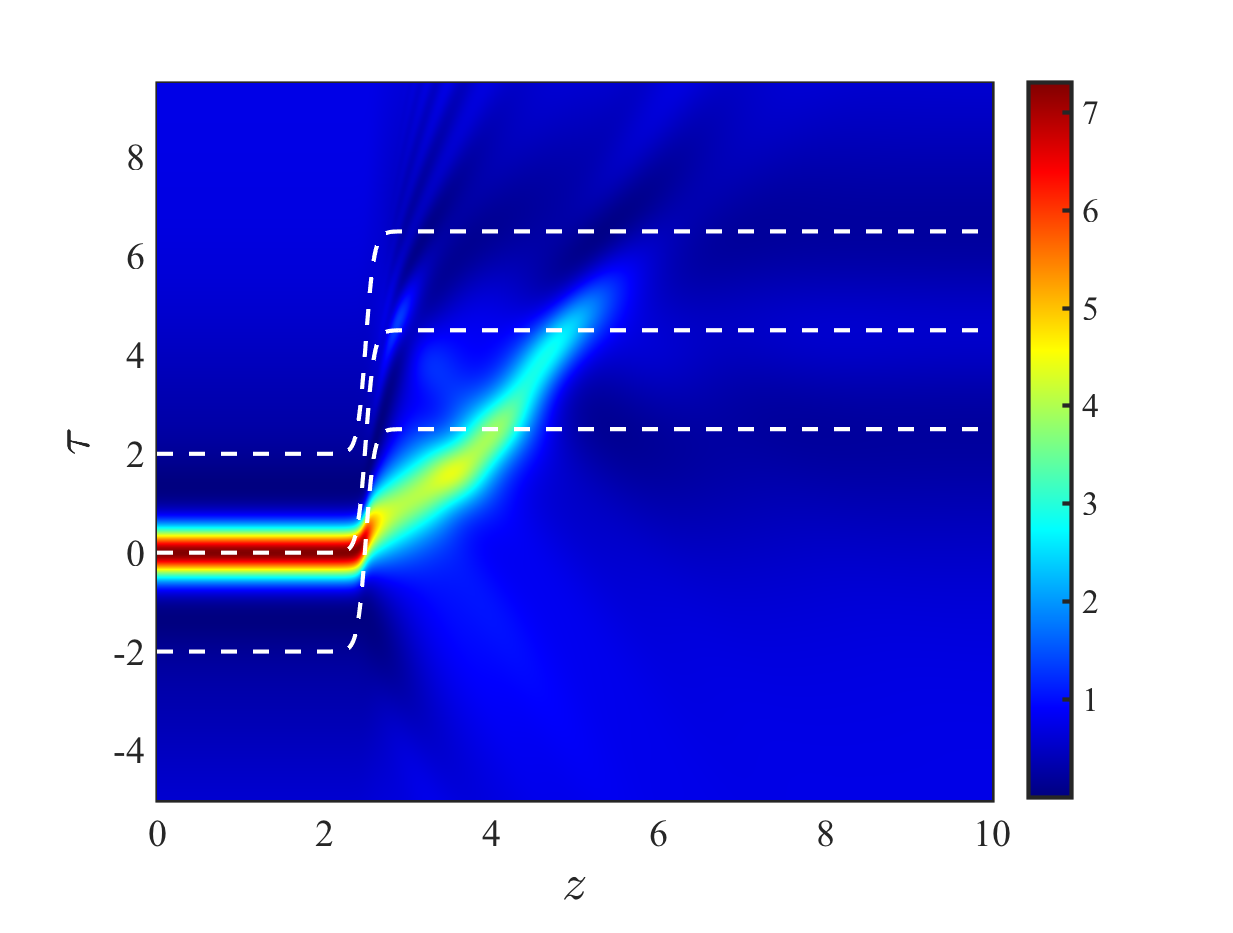
\includegraphics[width=0.5\textwidth]{regularDensity5v2.eps}  \\
\vspace{-0.5em}
\hspace{2em}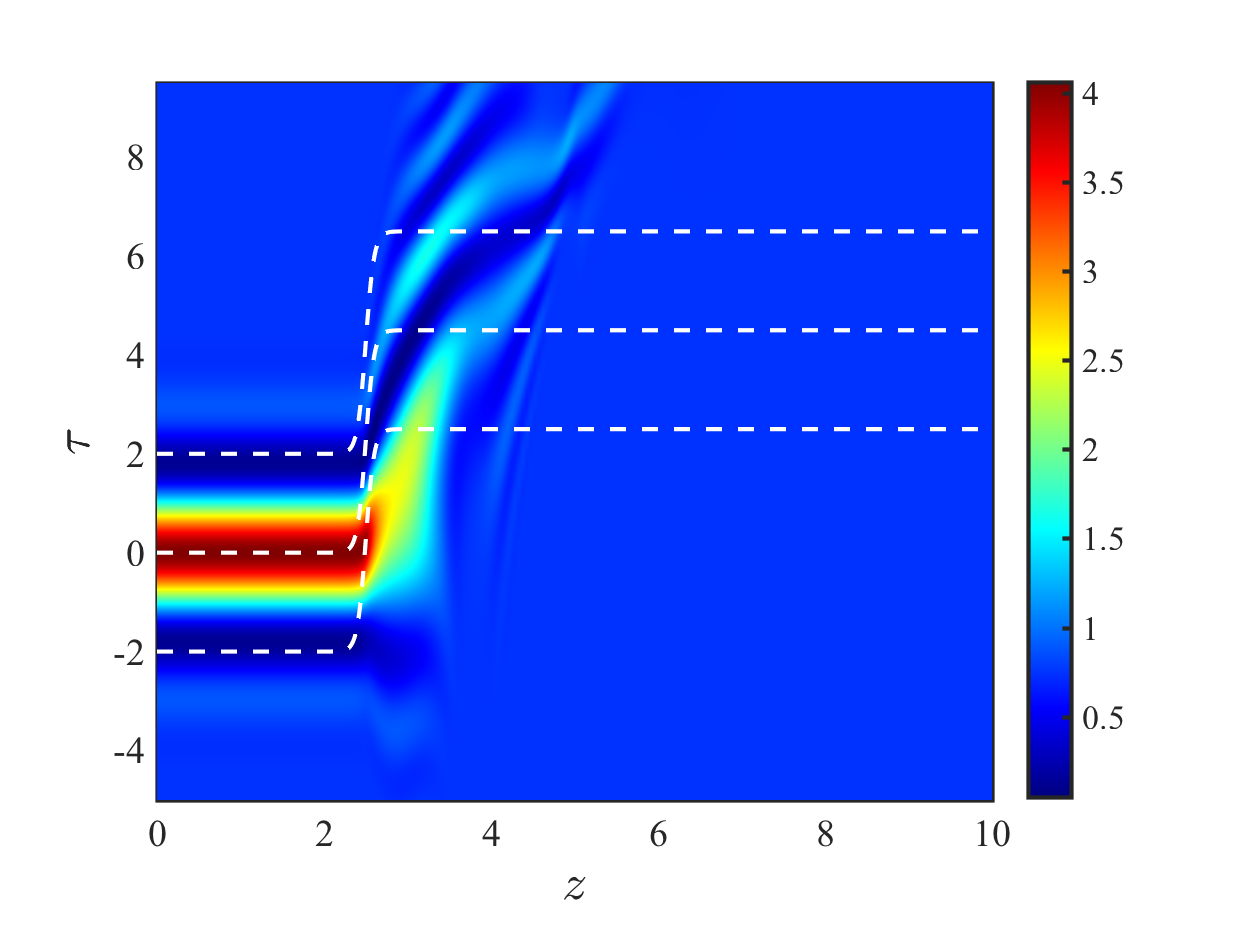
\includegraphics[width=0.5\textwidth]{regularNCVADensity5v2.eps} 
\end{figure}
\end{column}
\begin{column}{0.5\textwidth}
\vspace{-0.5em} \raggedright
\hspace{-2em}\includemedia[%
 		width=0.9\linewidth,%
		transparent=true,%
  		activate=onclick,%
		deactivate=pageclose,%
  		addresource=regular5.mp4,%
  		flashvars={source=regular5.mp4 &loop=true &controlBarAutoHide=true}%
		]{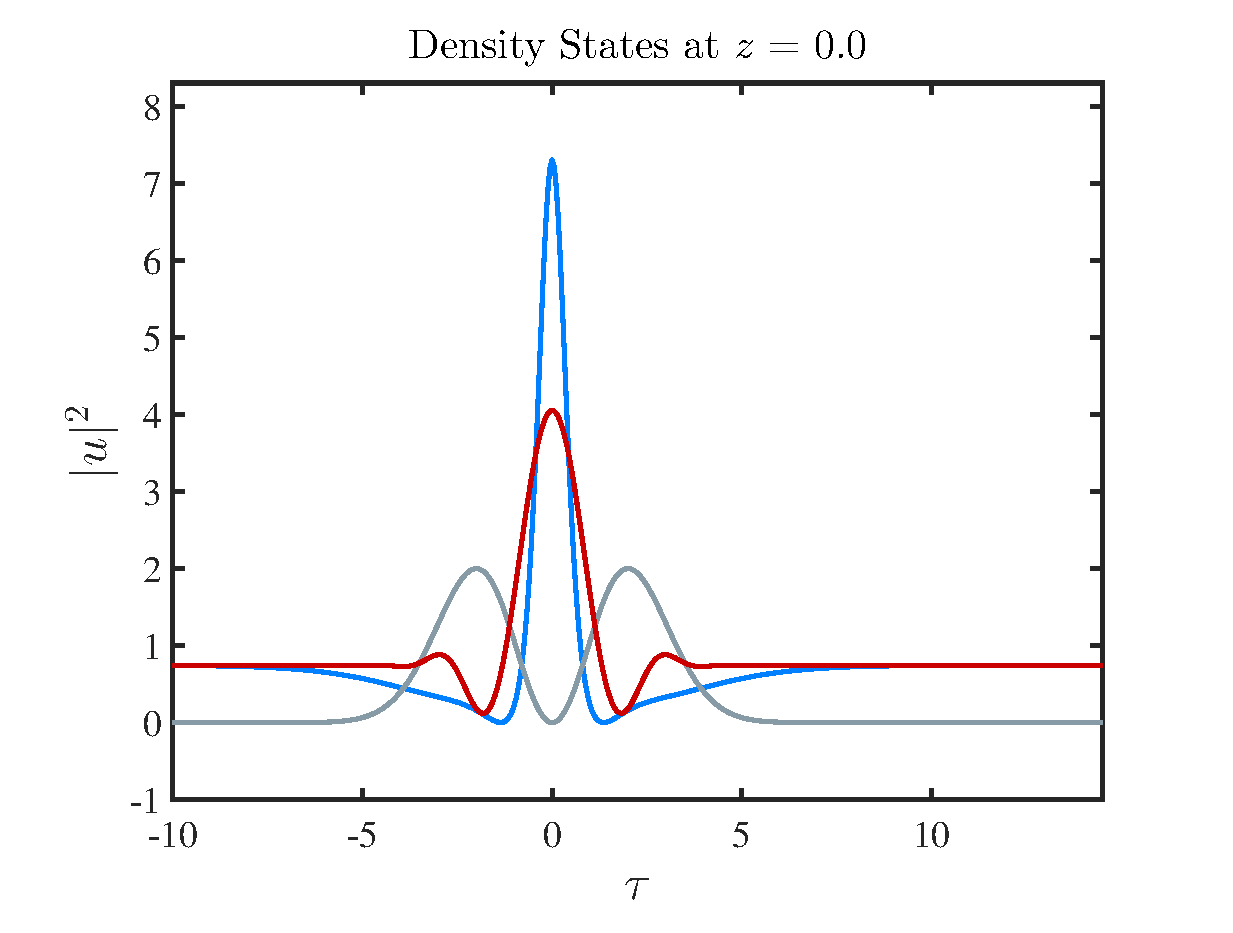
\includegraphics[width=0.5\textwidth]{regular5.eps}}{VPlayer.swf}%{StrobeMediaPlayback.swf}
\end{column}
\end{columns}
\end{column}
\end{columns}
\end{frame}

%Slide Natural 2
\begin{frame}[c]{Applications: Temporal Tweezing of Light}{\textcolor{paleblue}{Natural Width Tweezer} ($\sigma_\phi = 2$ and $h_\phi  = 4.6633$ )}

\begin{columns}

\begin{column}{0.28\textwidth}

\vspace{-7em}
\begin{framed}
\vspace{-1em}
\begin{figure}[h]
\centering
\centerline{\includegraphics[width=3cm]{RegularPDEvODE_rcg_t.eps}\hspace*{0cm}}
\caption{\tiny $\delta Q$ Comparison LL Model and NCVA}
\end{figure}
\vspace{-1em}
\end{framed}
\end{column}
\vrule width 1pt

\begin{column}{0.75\textwidth}
\vspace{-0.5em}
\centering
{\small Non-Tweezed CS:  $\tau_f =12$, $\beta = 10$ }
\vspace{0.5em}
\begin{columns}
\begin{column}{0.5\textwidth}
\vspace{-1em}
\begin{figure}
\hspace{2em}\includegraphics[width=0.5\textwidth]{regularDensity3v2.eps}  \\
\vspace{-0.5em}
\hspace{2em}\includegraphics[width=0.5\textwidth]{regularNCVADensity3v2.eps} 
\end{figure}
\end{column}
\begin{column}{0.5\textwidth}
\vspace{-0.5em} \raggedright
\hspace{-2em}\includemedia[%
 		width=0.9\linewidth,%
		transparent=true,%
  		activate=onclick,%
		deactivate=pageclose,%
  		addresource=regular3.mp4,%
  		flashvars={source=regular3.mp4 &loop=true &controlBarAutoHide=true}%
		]{\includegraphics[width=0.5\textwidth]{regular3.eps}}{VPlayer.swf}%{StrobeMediaPlayback.swf}
\end{column}
\end{columns}
\vspace{0.5em}

\hrule width\textwidth 

\vspace{0.5em}
{\small Inlet:  $\tau_f =5.5$, $\beta = 8$ }
\begin{columns}
\begin{column}{0.5\textwidth}
\centering
\vspace{-1em}
\begin{figure}
\hspace{2em}\includegraphics[width=0.5\textwidth]{regularDensity6v2.eps}  \\
\vspace{-0.5em}
\hspace{2em}\includegraphics[width=0.5\textwidth]{regularNCVADensity6v2.eps} 
\end{figure}
\end{column}
\begin{column}{0.5\textwidth}
\vspace{-0.5em} \raggedright
\hspace{-2em}\includemedia[%
 		width=0.9\linewidth,%
		transparent=true,%
  		activate=onclick,%
		deactivate=pageclose,%
  		addresource=regular6.mp4,%
  		flashvars={source=regular6.mp4 &loop=true &controlBarAutoHide=true}%
		]{\includegraphics[width=0.5\textwidth]{regular6.eps}}{VPlayer.swf}%{StrobeMediaPlayback.swf}
\end{column}
\end{columns}
\end{column}
\end{columns}
\end{frame}

%Slide  Wide 1
\begin{frame}[c]{Applications: Temporal Tweezing of Light}{\textcolor{paleblue}{Wide Width Tweezer} ($\sigma_\phi = 3$ and $h_\phi  = 6.9949$ )}

\begin{columns}

\begin{column}{0.28\textwidth}

\vspace{-7em}
\begin{framed}
\vspace{-1em}
\begin{figure}[h]
\centering
\centerline{\includegraphics[width=3cm]{FatPDEvODE_rcg_t.eps}\hspace*{0cm}}
\caption{\tiny $\delta Q$ Comparison LL Model and NCVA}
\end{figure}
\vspace{-1em}
\end{framed}
\end{column}
\vrule width 1pt

\begin{column}{0.75\textwidth}
\vspace{-0.5em}
\centering
{\small LL Tweezed CS/ NCVA no-CS:  $\tau_f =4$, $\beta = 10$ }
\vspace{0.5em}
\begin{columns}
\begin{column}{0.5\textwidth}
\vspace{-1em}
\begin{figure}
\hspace{2em}\includegraphics[width=0.5\textwidth]{fatDensity1v2.eps}  \\
\vspace{-0.5em}
\hspace{2em}\includegraphics[width=0.5\textwidth]{fatNCVADensity1v2.eps} 
\end{figure}
\end{column}
\begin{column}{0.5\textwidth}
\vspace{-0.5em} \raggedright
\hspace{-2em}\includemedia[%
 		width=0.9\linewidth,%
		transparent=true,%
  		activate=onclick,%
		deactivate=pageclose,%
  		addresource=fat1.mp4,%
  		flashvars={source=fat1.mp4 &loop=true &controlBarAutoHide=true}%
		]{\includegraphics[width=0.5\textwidth]{fat1.eps}}{VPlayer.swf}%{StrobeMediaPlayback.swf}
\end{column}
\end{columns}
\vspace{0.5em}

\hrule width\textwidth 

\vspace{0.5em}
{\small No-CS:  $\tau_f =5.5$, $\beta = 10$ }
\begin{columns}
\begin{column}{0.5\textwidth}
\centering
\vspace{-1em}
\begin{figure}
\hspace{2em}\includegraphics[width=0.5\textwidth]{fatDensity2v2.eps}  \\
\vspace{-0.5em}
\hspace{2em}\includegraphics[width=0.5\textwidth]{fatNCVADensity2v2.eps} 
\end{figure}
\end{column}
\begin{column}{0.5\textwidth}
\vspace{-0.5em} \raggedright
\hspace{-2em}\includemedia[%
 		width=0.9\linewidth,%
		transparent=true,%
  		activate=onclick,%
		deactivate=pageclose,%
  		addresource=fat2.mp4,%
  		flashvars={source=fat2.mp4 &loop=true &controlBarAutoHide=true}%
		]{\includegraphics[width=0.5\textwidth]{fat2.eps}}{VPlayer.swf}%{StrobeMediaPlayback.swf}
\end{column}
\end{columns}
\end{column}
\end{columns}
\end{frame}

%Slide  Wide 2
\begin{frame}[c]{Applications: Temporal Tweezing of Light}{\textcolor{paleblue}{Wide Width Tweezer} ($\sigma_\phi = 3$ and $h_\phi  = 6.9949$ )}

\begin{columns}

\begin{column}{0.28\textwidth}

\vspace{-7em}
\begin{framed}
\vspace{-1em}
\begin{figure}[h]
\centering
\centerline{\includegraphics[width=3cm]{FatPDEvODE_rcg_t.eps}\hspace*{0cm}}
\caption{\tiny $\delta Q$ Comparison LL Model and NCVA}
\end{figure}
\vspace{-1em}
\end{framed}
\end{column}
\vrule width 1pt

\begin{column}{0.75\textwidth}
\vspace{-0.5em}
\centering
{\small Non-Tweezed CS:  $\tau_f =18$, $\beta = 10$ }
\vspace{0.5em}
\begin{columns}
\begin{column}{0.5\textwidth}
\vspace{-1em}
\begin{figure}
\hspace{2em}\includegraphics[width=0.5\textwidth]{fatDensity3v2.eps}  \\
\vspace{-0.5em}
\hspace{2em}\includegraphics[width=0.5\textwidth]{fatNCVADensity3v2.eps} 
\end{figure}
\end{column}
\begin{column}{0.5\textwidth}
\vspace{-0.5em} \raggedright
\hspace{-2em}\includemedia[%
 		width=0.9\linewidth,%
		transparent=true,%
  		activate=onclick,%
		deactivate=pageclose,%
  		addresource=fat3.mp4,%
  		flashvars={source=fat3.mp4 &loop=true &controlBarAutoHide=true}%
		]{\includegraphics[width=0.5\textwidth]{fat3.eps}}{VPlayer.swf}%{StrobeMediaPlayback.swf}
\end{column}
\end{columns}
\vspace{0.5em}

\hrule width\textwidth 

\vspace{0.5em}
{\small Inlet:  $\tau_f =9$, $\beta = 10$ }
\begin{columns}
\begin{column}{0.5\textwidth}
\centering
\vspace{-1em}
\begin{figure}
\hspace{2em}\includegraphics[width=0.5\textwidth]{fatDensity5v2.eps}  \\
\vspace{-0.5em}
\hspace{2em}\includegraphics[width=0.5\textwidth]{fatNCVADensity5v2.eps} 
\end{figure}
\end{column}
\begin{column}{0.5\textwidth}
\vspace{-0.5em} \raggedright
\hspace{-2em}\includemedia[%
 		width=0.9\linewidth,%
		transparent=true,%
  		activate=onclick,%
		deactivate=pageclose,%
  		addresource=fat5.mp4,%
  		flashvars={source=fat5.mp4 &loop=true &controlBarAutoHide=true}%
		]{\includegraphics[width=0.5\textwidth]{fat5.eps}}{VPlayer.swf}%{StrobeMediaPlayback.swf}
\end{column}
\end{columns}
\end{column}
\end{columns}
\end{frame}

%Slide
\begin{frame}{Applications: Temporal Tweezing of Light}{Numerical Simulation: \textcolor{paleblue}{Natural Width Tweezer}}
\raggedright {Variable $\tau_f$ and $\beta$}
\centering
\begin{columns}
\begin{column}{0.45\textwidth}
\centering
\vspace{-2em}
\begin{figure}
\hspace{2em}\includegraphics[width=0.9\textwidth]{regularDensityFinal.eps}  \\
\vspace{-1.4em}
\hspace{2em}\includegraphics[width=0.9\textwidth]{regularNCVADensityFinal.eps} 
\end{figure}
\end{column}
\begin{column}{0.55\textwidth}
\vspace{1.5em} \raggedright
\hspace{-2em}\includemedia[%
 		width=\linewidth,%
		transparent=true,%
  		activate=onclick,%
		deactivate=pageclose,%
  		addresource=final.mp4,%
  		flashvars={source=final.mp4 &loop=true &controlBarAutoHide=true}%
		]{\includegraphics[width=0.5\textwidth]{final.eps}}{VPlayer.swf}%{StrobeMediaPlayback.swf}
\end{column}
\end{columns}

\end{frame}

%Conclusions
\begin{frame}
\frametitle{Conclusion}
\begin{block}{}
\begin{itemize}
\item Applied Non-conservative Variational Technique for complex PDEs
\begin{itemize}
\item  \textcolor{paleblue}{Advantage}:  Reduce infinite-dimensional PDE to finite-dimensional ODE 
\item  \textcolor{regal}{Disadvantage}:  Ansatz and its subspace
\item  \textcolor{paleblue}{Advantage}:  Isolate changes of state i.e. bifurcations
\item  \textcolor{regal}{Disadvantage}:  NCVA may be overly cumbersome
\end{itemize}
\item PVA = NCVA 
%\pause 
\item Exciton-polariton condensates 
\item Found SSB bifurcations in coherently-driven passive optical Kerr resonator
\item Describe tweezers for temporally tweezed CS stored in a passive loop of optical fiber
%\pause 
%\item Stability of Parameters 
%%\pause 
%\item Need Good Ansatz for VA

\end{itemize}
\end{block}
\end{frame}


% Future Research
\begin{frame}
\frametitle{Future Research}
\begin{block}{}
\begin{itemize}
%\item \textcolor{paleblue}{Reverse} Pitchfork Bifurcation
%\item \textcolor{paleblue} {Dynamics} for Spontaneous Symmetry Breaking 
%\item \textcolor{paleblue}{Quartic} Phase Terms to Ansatz 
%\item Defocusing NLS Equation 
\item Exciton-polariton Condensates
\begin{itemize}
\item  Bright and dark soliton dynamics 
\item Boundaries of \textcolor{paleblue}{stability inversion}
\item  \textcolor{paleblue}{Two-dimensional} GPE nodeless clouds and single vortex
%\item  \textcolor{paleblue}{Bright solitons} (BSs) and BS-BS  \textcolor{paleblue}{interactions} 
\end{itemize}
\item Further Applications: \textcolor{paleblue} {Temporal Tweezing of Light} add interactions of multiple CSs for optical information processing
\item Apply NCVA to \textcolor{paleblue}{Ginzburg-Landau equations}
%modeling 
 %nonlinear waves, phase transitions,
%superconductors and superfluids,
%\item  Bright and dark soliton dynamics with \textcolor{paleblue}{phenomenological dissipation}
%\item Further Applications: \textcolor{paleblue} {Temporal Tweezing of Light} 
\end{itemize}
\end{block}

\end{frame}

%Slide
\begin{frame}
\frametitle{Acknowledgements}
\begin{columns}
\begin{column}{0.5\textwidth}
Advisor 
\begin{itemize}
\item Prof. Ricardo Carretero 
\end{itemize}

Research Collaborators 
\begin{itemize}
\item Dr. Panos Kevrekidis
\item Dr. Mariana Haragus
\end{itemize}
\end{column}
\begin{column}{0.5\textwidth}
Dissertation Committee Members
\begin{itemize}
\item Dr. Ali Nadim
\item Dr. Marina Chugunova
\item Dr. Michael Bromley
\item Dr. Christopher Curtis 
\end{itemize}
\end{column}
\end{columns}
Support
\begin{columns}
\begin{column}{0.3\textwidth}
%\begin{itemize}
%\item 
\centering 
\includegraphics[height= 0.15\textheight]{CSRC.png}
%\end{itemize}
\end{column}
\begin{column}{0.3\textwidth}
%\begin{itemize}
%\item 
\centering
\includegraphics[height= 0.15\textheight]{ARCS.png}
%\end{itemize}
\end{column}
\begin{column}{0.3\textwidth}
%\begin{itemize}
%\item  
\centering
\includegraphics[width = 0.75\linewidth]{Cymer.png}
%\end{itemize}
\end{column}
\end{columns}

\begin{alertblock} {Thank You for Listening!}
  Questions? 
\end{alertblock}
\end{frame}

%Slide
\begin{frame}[c]{Applications: Temporal Tweezing of Light}{\textcolor{paleblue}{Narrow Width Tweezer} ($\sigma_\phi = 1$ and $h_\phi  = 2.3316$ )}

\begin{columns}

\begin{column}{0.28\textwidth}

\vspace{-7em}
\hskip -0.5cm \begin{framed}
\vspace{-1em}
\begin{figure}[h]
%\hspace{-1.05em}
%\hskip -0.43108cm 
\centering
\centerline{
\includegraphics[width=3cm]{SkinnyPDEvODE_rcg_t.eps}\hspace*{0.2cm}}

\caption{\tiny $\delta Q$ Comparison LL Model and NCVA}
\end{figure}
\vspace{-1.5em}
\end{framed}
\end{column}
\vrule width 1pt

\begin{column}{0.75\textwidth}
\vspace{-0.5em}
\centering
{\small Tweezed CS:  $\tau_f =0.1$, $\beta = 0.1$ }
\vspace{0.5em}
\begin{columns}
\begin{column}{0.5\textwidth}
\vspace{-1em}
\begin{figure}
\hspace{2em}\includegraphics[width=0.5\textwidth]{skinnyDensity1v2.eps}  \\
\vspace{-0.5em}
\hspace{2em}\includegraphics[width=0.5\textwidth]{skinnyNCVADensity1v2.eps} 
\end{figure}
\end{column}
\begin{column}{0.5\textwidth}
\vspace{-0.5em} \raggedright
\hspace{-2em}\includemedia[%
 		width=0.9\linewidth,%
		transparent=true,%
  		activate=onclick,%
		deactivate=pageclose,%
  		addresource=skinny1.mp4,%
  		flashvars={source=skinny1.mp4 &loop=true &controlBarAutoHide=true}%
		]{\includegraphics[width=0.5\textwidth]{skinny1.eps}}{VPlayer.swf}%{StrobeMediaPlayback.swf}
\end{column}
\end{columns}
\vspace{0.5em}
\hrule width\textwidth 

\vspace{0.5em}
{\small No-CS:  $\tau_f =2$, $\beta = 10$ }
\begin{columns}
\begin{column}{0.5\textwidth}
\centering
\vspace{-1em}
\begin{figure}
\hspace{2em}\includegraphics[width=0.5\textwidth]{skinnyDensity3v2.eps}  \\
\vspace{-0.5em}
\hspace{2em}\includegraphics[width=0.5\textwidth]{skinnyNCVADensity3v2.eps} 
\end{figure}
\end{column}
\begin{column}{0.5\textwidth}
\vspace{-0.5em} \raggedright
\hspace{-2em}\includemedia[%
 		width=0.9\linewidth,%
		transparent=true,%
  		activate=onclick,%
		deactivate=pageclose,%
  		addresource=skinny2.mp4,%
  		flashvars={source=skinny2.mp4 &loop=true &controlBarAutoHide=true}%
		]{\includegraphics[width=0.5\textwidth]{skinny2.eps}}{VPlayer.swf}%{StrobeMediaPlayback.swf}
\end{column}
\end{columns}
\end{column}
\end{columns}
\end{frame}





%\begin{frame}

%\begin{block}{References}
%\tiny{
%\bibliographystyle{../mio}
%\bibliography{../references}
%}
%\end{block}
%\end{frame}

% \begin{frame}{test}
% 	Main text still in Gill Sans
% 	$$\frac{f}{f^4}$$
% 	
% 	But math is now different
% 	\Large
% 	$$\frac{f^2}{f^4}$$
% \end{frame}


\end{document}

